\documentclass[]{report}
%% Useful packages
\usepackage[utf8]{inputenc}
\usepackage[a4paper,left=2cm,right=2cm,top=2cm,bottom=2cm]{geometry}
\usepackage{crop,graphicx,amsmath,array,color,amssymb,fancyhdr,lineno,float,booktabs}
\usepackage{flushend,stfloats,amsthm,chngpage,times,,lipsum,lastpage,parskip} 
\usepackage{calc,listings,color,wrapfig,tabularx,longtable,multirow,enumitem,commath,siunitx}
\usepackage[table,xcdraw]{xcolor}
\usepackage[font=itshape]{quoting}
%\usepackage[numbers]{natbib}
%\usepackage[subtle]{savetrees}
\usepackage[
  nottoc
  %notlot
  %notlof
]{tocbibind}

\usepackage{titlesec}

\titleformat{\chapter}[display]
{\normalfont\huge\bfseries}{\chaptertitlename\ \thechapter}{20pt}{\Huge}

% this alters "before" spacing (the second length argument) to 0
\titlespacing*{\chapter}{0pt}{0pt}{40pt}

\usepackage{hyperref}
\hypersetup{
    colorlinks=true,
    linkcolor=black,
    filecolor=teal,      
    urlcolor=teal,
    citecolor=teal,
    pdftitle={CEGE0016 Topic Notes},
    pdfauthor={HD},
}

\renewcommand\bibname{References}
\usepackage{lineno}
%%%%%%%%%%%%   Header and Footer  %%%%%%%%%%%%%
\pagestyle{fancy}
\title{%
  Topic Notes}
\author{HD
}

\begin{document}
\begin{titlepage}

  \newcommand{\HRule}{\rule{\linewidth}{0.5mm}} % Defines a new command for the horizontal lines, change thickness here

  %----------------------------------------------------------------------------------------
  %	LOGO SECTION
  %----------------------------------------------------------------------------------------
  \center
  
\includegraphics[width=5cm]{Title/UCL.png}\\[1cm] % Include a department/university logo - this will require the graphicx package

  %----------------------------------------------------------------------------------------

  \center % Center everything on the page

  %----------------------------------------------------------------------------------------
  %	HEADING SECTIONS
  %----------------------------------------------------------------------------------------

  \textsc{\LARGE University College London }\\[1.5cm] % Name of your university/college
  \textsc{\Large MEng Mechanical Engineering  }\\[0.5cm] % Major heading such as course name
  \textsc{\large MECH0071 Electrical Power Systems and Electrical Propulsion }\\[1.5cm] % Minor heading such as course title

  %----------------------------------------------------------------------------------------
  %	TITLE SECTION
  %----------------------------------------------------------------------------------------
  \makeatletter
  { \huge \textsc \@title}\\[1.5cm] % Title of your document


  %----------------------------------------------------------------------------------------
  %	AUTHOR SECTION
  %----------------------------------------------------------------------------------------

  \begin{minipage}{0.4\textwidth}
    \begin{flushleft} \large
      \emph{Author:}\\
      \@author % Your name
      \\[1.2em]
      %\emph{ID No:}\\
      %0101010 \\[1.2em]
    \end{flushleft}
  \end{minipage}
  ~
  \begin{minipage}{0.4\textwidth}
    \begin{flushright} \large
      \emph{Module coordinator:} \\
      Prof. Richard Bucknall \\[1.2em] % Supervisor's Name
      %\emph{Module teaching team:} \\
      %Dr. Tim Hillel\\ % second marker's name
      %Mr. Umut Lagap
    \end{flushright}
  \end{minipage}\\[2cm]
  \makeatother

  % If you don't want a supervisor, uncomment the two lines below and remove the section above
  %\Large \emph{Author:}\\
  %John \textsc{Smith}\\[3cm] % Your name

  %----------------------------------------------------------------------------------------
  %	DATE SECTION
  %----------------------------------------------------------------------------------------

  {\large \today}\\[2cm] % Date, change the \today to a set date if you want to be precise

  \vfill % Fill the rest of the page with whitespace

\end{titlepage}

\fancyhf{}
\fancyhead[L]{CEGE0016}
\fancyfoot[L]{HD}
\fancyfoot[R]{ \bf\thepage\ \rm }%

\fancypagestyle{plain}{%
  \fancyhf{}%
  \fancyfoot[L]{HD}
  \fancyfoot[R]{ \bf\thepage\ \rm }%
  \renewcommand{\headrulewidth}{0pt}% Line at the header invisible
  \renewcommand{\footrulewidth}{0pt}% Line at the footer visible
}

\newpage
\tableofcontents
\newpage
\listoffigures
\listoftables
\newpage

\documentclass[class=report, crop=false, 12pt,a4paper]{standalone}
\usepackage{enumitem}
\usepackage{multicol}
\usepackage{graphicx}
\usepackage{float}
\usepackage{amsmath}
\usepackage{amssymb}
\usepackage{mathtools}
\usepackage{siunitx}
\usepackage{commath}
\usepackage{array}
\usepackage{natbib}
\usepackage[a4paper,width=150mm,top=25mm,bottom=25mm]{geometry}
\setlength{\parindent}{0pt}
\begin{document}
\chapter{Module Introduction}
\section{Teaching Team}
\begin{itemize}
	\item Dr Gemma Cremen - Lecture in Resilience Engineering, Module Coordinator
	      \begin{itemize}
		      \item g.cremen@ucl.ac.uk
	      \end{itemize}
	\item Dr Tim Hillel - Lecturer in Analytics of Infrastructure Systems, Deputy Module Coordinator
	      \begin{itemize}
		      \item tim.hillel@ucl.ac.uk
	      \end{itemize}
	\item Mr Umut Lagap - PhD Student in Risk and Resilience, PGTA
	      \begin{itemize}
		      \item umut.lagap.21@ucl.ac.uk
	      \end{itemize}
\end{itemize}
\section{Assessment}
\begin{figure}[H]
	\centering
	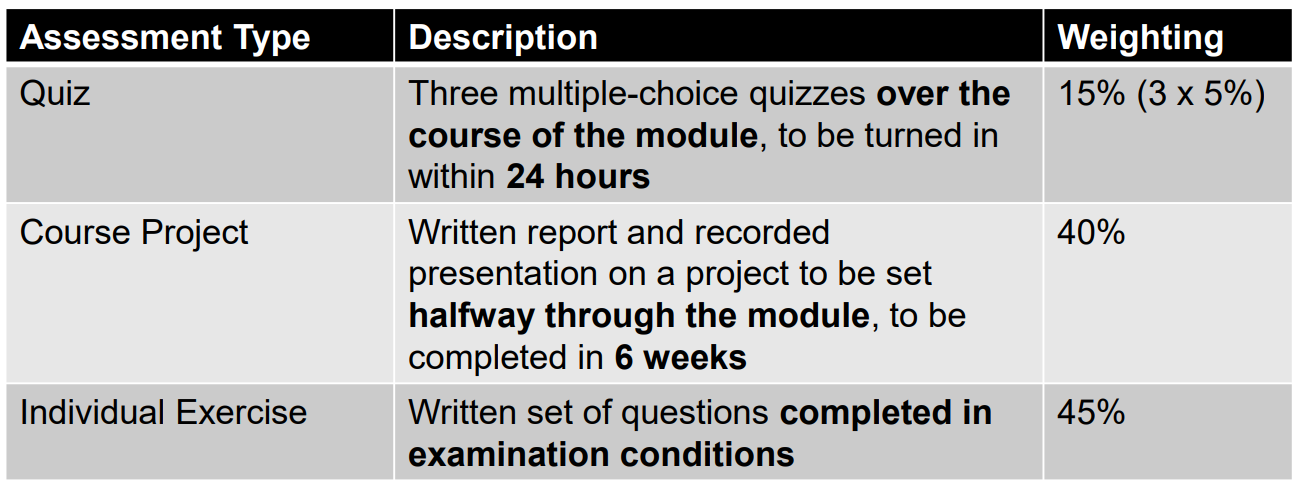
\includegraphics[width = 0.9 \textwidth]{../img/figure1.png}
	\caption{Module Assessment.}
\end{figure}
\section{Timeline}
\begin{figure}[H]
	\centering
	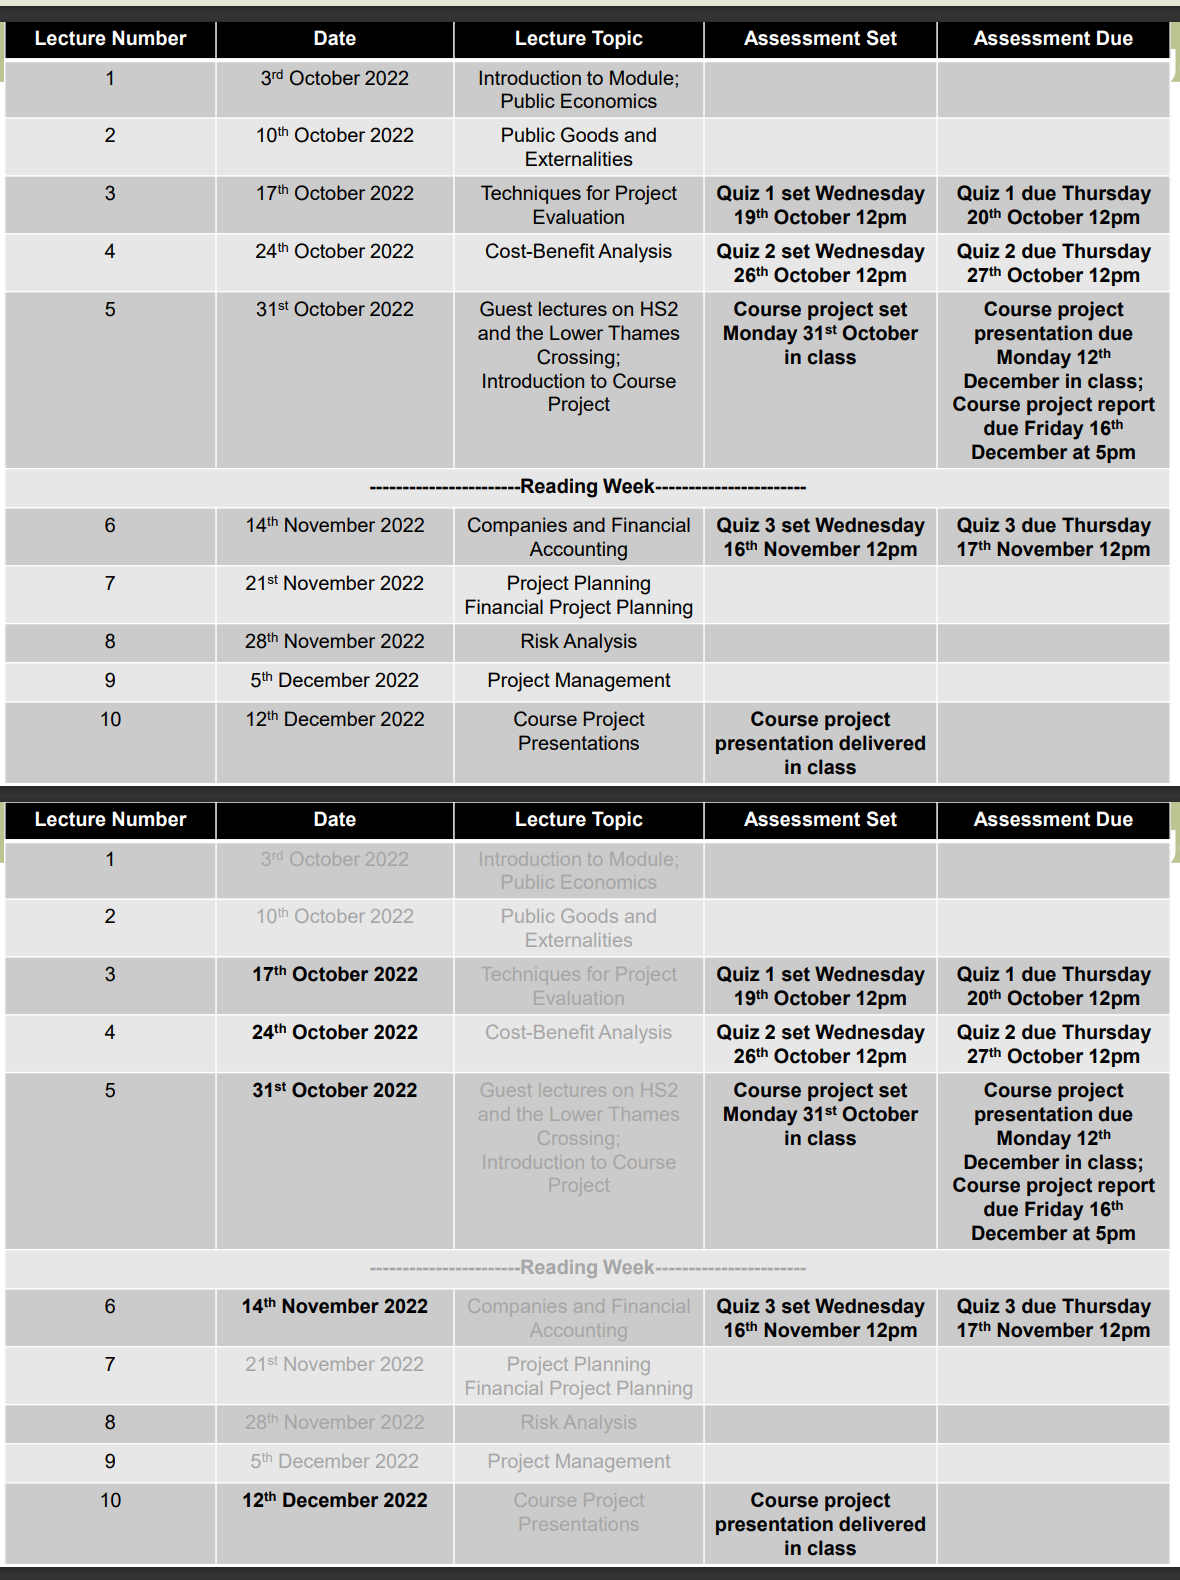
\includegraphics[width = 0.9 \textwidth]{../img/figure2.png}
	\caption{Module Timeline.}
\end{figure}
\chapter{Introduction to public economics}
\section{Introduction and overview of mixed economies}
\subsection{Aims}
\begin{enumerate}
	\item Understand the roles of the private and public sector in mixed economies
	\item Become (re)familiar with key microeconomic concepts of consumption and production, including Pareto optimality and market equilibrium
	\item Understand the trade-offs between market efficiency and equitable distribution of resources
	\item Be aware of the assumptions and limitations of fundamental theorems and associated neoclassical economics
\end{enumerate}
\subsection{Economies}
\subsubsection{A simplified definition}
\begin{quote}
	An area of \textit{production, trade} and \textit{consumption} of goods and services by different \textit{agents}.
\end{quote}
\subsubsection{Agents}
\begin{itemize}
	\item Individuals and households
	\item Businesses
	\item Government
\end{itemize}
\subsection{Mixed economies}
\subsubsection{Economies today are predominantly \textit{mixed economies}}
Private sector:
\begin{quote}
	profit-maximising firms operate in competitive markets
\end{quote}
Public sector:
\begin{quote}
	governments/other organisations make interventions in those markets
\end{quote}
\subsection{Private sector}
\subsubsection{Welfare economics}
\begin{quote}
	"he is in this, as in many other cases, led by an invisible hand to promote an end which has no part of his intention. Nor is it always the worse for the society that it was no part of it. By pursuing his own interest he frequently promotes that of the society more effectively than when he really intends to promote it. (Smith 1776)
\end{quote}
\subsection{Public sector}
\subsubsection{Public sector aims to balance trade-offs}
In particular
\begin{quote}
	efficiency of competitive markets vs. improved equity of distribution of income from regulation
\end{quote}
Understanding the role of public sector in mixed economies first requires u s to understand operation of free-markets
\subsection{Classical microeconomics}
\begin{figure}[H]
	\centering
	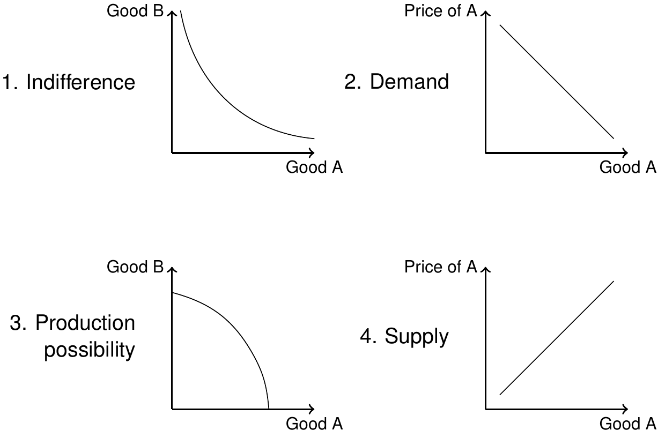
\includegraphics[width = 0.9 \textwidth]{../img/figure3.png}
	\caption{Classical microeconomic models.}
\end{figure}
\subsection{Economic models}
\begin{quote}
	"Remember that all models are wrong; the practical question is how wrong do they have to be to not be useful" (Box and Draper 1987)
\end{quote}
\section{Consumer theory}
\subsection{Consumer theory: continuous goods}
\begin{itemize}
	\item $J$ continuous goods, each good denoted by $j = 1, \, ..., \, J$
	\item Each good has associated price per unit $p_j$
	      \begin{itemize}
		      \item e.g., $j = 1$ corresponds to milk, $p_j = \SI{90}{pence\per litre}$
		      \item $j = 2$ corresponds to eggs, $p_j = \SI{16}{pence \per egg}$
	      \end{itemize}
	\item Consider choice of agent, with total budget $I$
	      \begin{itemize}
		      \item Assume agent represents individual
		      \item Individual chooses quantity $q_j$ of each good $j$, subject to budget constraint
	      \end{itemize}
\end{itemize}
\begin{gather}
	\sum_{j=1}^{J} \left(p_jq_j\right) \leq I
\end{gather}
\subsection{Utility}
\begin{itemize}
	\item Individual's choice of goods represented by consumption bundle $Q$
	      \begin{itemize}
		      \item i.e. vector of $q_1, \, ..., \, q_J$
	      \end{itemize}
	\item Individual gets utility $U\left(Q\right)$ from $Q$
	      \begin{itemize}
		      \item Utility represents how individuals perceived benefit from consuming/owning $Q$
		      \item Assume $U\left(Q\right)$ increases monotonically with increasing $q_i$
	      \end{itemize}
\end{itemize}
\subsection{Choice between two continuous goods}
\begin{figure}[H]
	\centering
	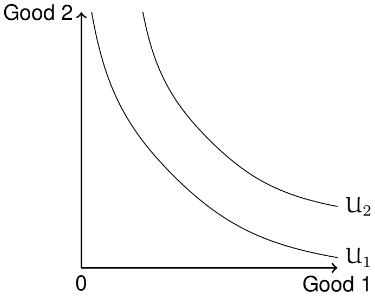
\includegraphics[width = 0.5\textwidth]{../img/figure4.png}
	\caption{}
\end{figure}
Indifference curves:
\begin{quote}
	Different combinations of each good that yield same level of utility
\end{quote}
Marginal Rate of Substitution (MRS):
\begin{quote}
	Gradient of indifference curve
\end{quote}
\begin{itemize}
	\item i.e. how many unites of good 2 individual would substitute for 1 unit of good 1
	\item Assumed to be convex
\end{itemize}
\subsection{Utility maximisation with budget constraint}
\begin{figure}[H]
	\centering
	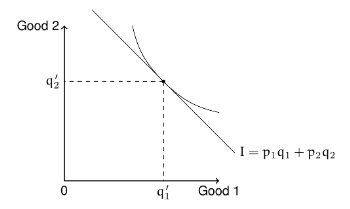
\includegraphics[width = 0.5\textwidth]{../img/figure5.png}
	\caption{}
\end{figure}
\begin{itemize}
	\item Assume agents try to maximise utility
	\item Under maximal utility assumption, optimal solution when indifference curve is tangent to budget line
\end{itemize}
\begin{gather}
	\textrm{MRS} = \dfrac{p_1}{p_2}
\end{gather}
\subsection{Trade between two agents}
\begin{figure}[H]
	\centering
	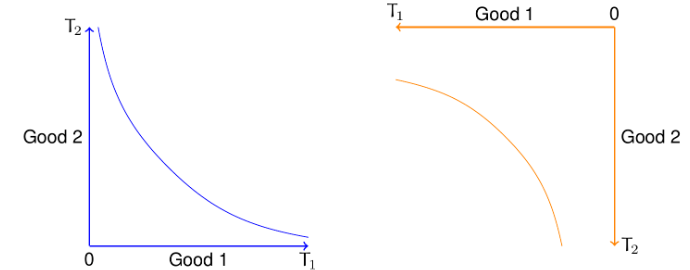
\includegraphics[width = \textwidth]{../img/figure6.png}
	\caption{}
\end{figure}
\subsection{Edgeworth box}
\begin{figure}[H]
	\centering
	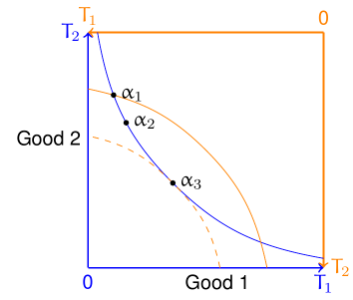
\includegraphics[width =0.5 \textwidth]{../img/figure7.png}
	\caption{}
\end{figure}
Edgeworth box:
\begin{quote}
	depicts distribution of commodities in closed economy between two agents
\end{quote}
Pareto improvement:
\begin{quote}
	A reallocation that improves utility of of one individual without reducing anyone else's utility
\end{quote}
\begin{itemize}
	\item $\alpha_2$ is Pareto improvement of $\alpha_1$
	\item $\alpha_3$ is Pareto improvement of $\alpha_2$
\end{itemize}
Pareto optimal/efficient:
\begin{quote}
	An allocation from which no-one can improve utility without reducing someone else's
\end{quote}
\begin{itemize}
	\item $\alpha_3$ is Pareto optimal
\end{itemize}
\subsection{Pareto efficiency}
\begin{itemize}
	\item Pareto efficient solutions happen when indifference curves have equal gradient
	\item i.e. each agent has equal MRS
\end{itemize}
Pareto frontier:
\begin{quote}
	Set of all possible Pareto efficient allocations
\end{quote}
\section{Producer theory}
\subsection{Production of goods and services}
\begin{figure}[H]
	\centering
	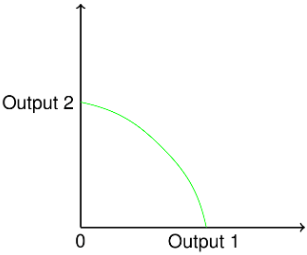
\includegraphics[width =0.5 \textwidth]{../img/figure8.png}
	\caption{}
\end{figure}
Production Possibilities Frontier (PPF):
\begin{quote}
	possible combinations of outputs (e.g. goods/services) that can be produced by economy with fixed inputs technology
\end{quote}
\begin{itemize}
	\item all points on PPF are production efficient: no more of one output can be produced without sacrificing the other
\end{itemize}
Marginal Rate of Transformation (MRT):
\begin{quote}
	Gradient of PPF
\end{quote}
\begin{itemize}
	\item Measures amount of Output 2 that must be sacrificed to produced additional unit of Output 1
\end{itemize}
\subsection{Marginal cost}
\begin{figure}[H]
	\centering
	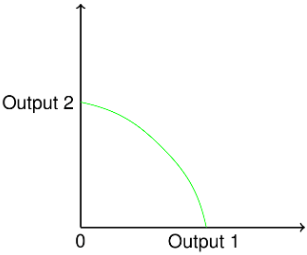
\includegraphics[width =0.5 \textwidth]{../img/figure8.png}
	\caption{}
\end{figure}
Marginal cost:
\begin{quote}
	Cost of producing one additional unit of output
\end{quote}
\begin{gather}
	\textrm{MRT} = \dfrac{MC_{output_1}}{MC_{output_2}}
\end{gather}
\begin{itemize}
	\item PPF often assumed to be concave under certain conditions (i.e. rewards diversity)
	      \begin{itemize}
		      \item Easier to obtain low-hanging fruit
	      \end{itemize}
\end{itemize}
\subsection{Pareto efficient production}
\begin{figure}[H]
	\centering
	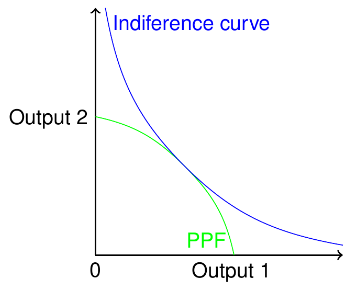
\includegraphics[width =0.5 \textwidth]{../img/figure9.png}
	\caption{}
\end{figure}
Pareto efficiency only achieved when production of goods matches consumers' willingness to pay
\begin{itemize}
	\item Gradient of PPF matches combined indifference curve of all consumers
	\item i.e. MRS = MRT
\end{itemize}
\subsection{Single market efficiency}
\begin{figure}[H]
	\centering
	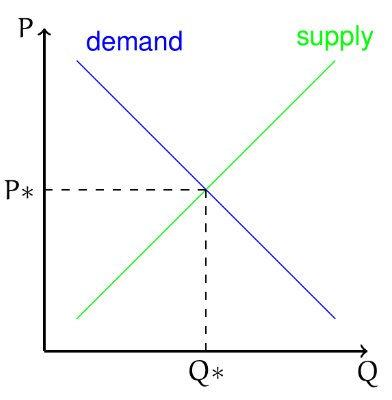
\includegraphics[width =0.5 \textwidth]{../img/figure10.png}
	\caption{}
\end{figure}
Market equilibrium occurs when supply equals demand
\begin{itemize}
	\item marginal benefit of consumption is equal to marginal cost of production
\end{itemize}
\section{Fundamental theorems of welfare economics}
\subsection{Competitive economies}
\subsubsection{Fundamental theorems of welfare economics}
If the economy is competitive, it is Pareto efficient
\subsection{Efficiency vs equality}
\begin{figure}[H]
	\centering
	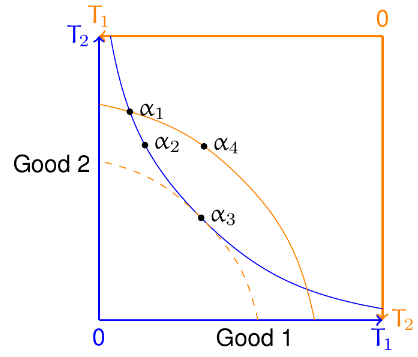
\includegraphics[width =0.5 \textwidth]{../img/figure11.png}
	\caption{}
\end{figure}
\begin{itemize}
	\item So far, considered only efficiency of allocations
	      \begin{itemize}
		      \item $\alpha_3$ is Pareto efficient
	      \end{itemize}
	\item Social welfare also depends on equitable distribution of goods
	\item How do we choose between $\alpha_3$ and $\alpha_4$
	      \begin{itemize}
		      \item Do we need to?
	      \end{itemize}
\end{itemize}
\subsection{Wealth distribution}
\subsubsection{Fundamental theorems of welfare economics}
\begin{itemize}
	\item If the economy is competitive, it is Pareto efficient
	\item Every Pareto efficient resource allocation can be obtained with competitive market process with an appropriate initial redistribution of wealth
\end{itemize}
\subsection{Efficiency and equality?}
\begin{figure}[H]
	\centering
	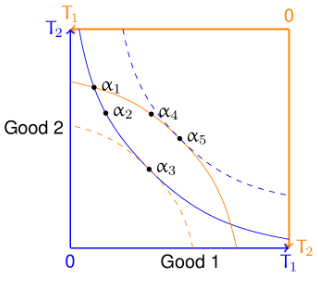
\includegraphics[width =0.5 \textwidth]{../img/figure12.png}
	\caption{}
\end{figure}
According to second fundamental theorem:
\begin{quote}
	more equitable allocation can be found through suitable assignment of initial endowments and free trade
\end{quote}
\section{Public sector}
\subsection{Role of government: the theory}
\subsubsection{When and how should governments make interventions in mixed economies?}
According to first fundamental theorem:
\begin{quote}
	government interventions that reduce competition make economies less efficient
\end{quote}
\begin{quote}
	Redistribute income and leave markets alone?
\end{quote}
\subsection{Role of government: reality}
Note\dots Governments play an active role in all major economies, including:
\begin{itemize}
	\item Allocation
	\item Distribution
	\item Regulation
	\item Stabilisation
\end{itemize}
\subsection{Market failures}
Several situations result in the failure of free markets to achieve optimal solutions. Causes include:
\begin{itemize}
	\item existence and need for public goods
	\item existence of externalities
	\item imperfect competition
	\item incomplete information and uncertainty
\end{itemize}
\section{Review and recap}
\subsection{A need for better understanding?}
\begin{itemize}
	\item Several strong assumptions
	      \begin{itemize}
		      \item Individuals as rational utility maximisers
		      \item Equivalence of utility, value and price
		      \item Markets as continuous
		      \item Statics tastes and preferences
		      \item Perfect competition
	      \end{itemize}
	\item Fundamental welfare economic theory does not capture
	      \begin{itemize}
		      \item unpaid labour
		      \item social exchange
		      \item long-term resilience and sustainability
	      \end{itemize}
\end{itemize}
\end{document}
\chapter{Public Goods and Externalities}
\section{Introduction}
\subsection{Aims}
\begin{enumerate}
  \item Recall the two dimensions of public good (rivalry and excludability) and understand how they lead to market failure
  \item Identify and describe the occurrence and results of positive and negative externalities
  \item Understand the role of the public sector in managing market failures arising from public goods and externalities
  \item Be aware of the particular challenges related to climate externalities
  \item Become familiar with the dimensions of the environmental ceiling and social foundations of the doughnut economic model
\end{enumerate}
\subsection{Market equilibrium}
Market equilibrium occurs when supply equals demand. Private marginal benefit of consumption is equal to private marginal cost of production.
\begin{figure}[H]
  \centering
  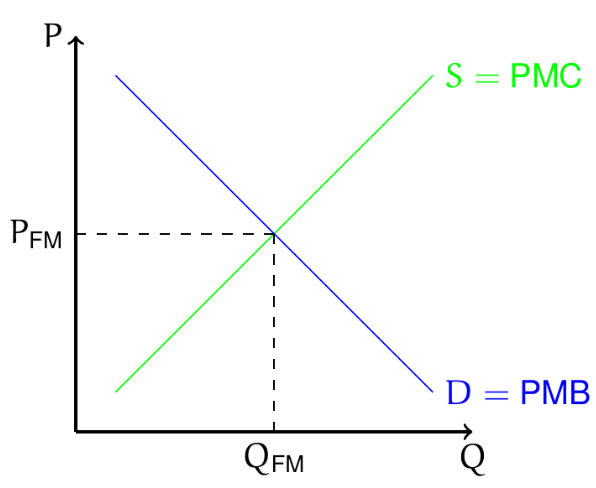
\includegraphics[width = 0.5\textwidth]{./img/figure13.png}
  \caption{Market equilibrium.}
\end{figure}
\subsection{Public goods and externalities}
\subsubsection{Definitions}
Public goods:
\begin{quote}
  Goods which are both non-excludable and have non rivalrous consumption.
\end{quote}
Externalities:
\begin{quote}
  Positive or negative effects on third parties arising from the production or consumption of goods, that are not reflected in the price
\end{quote}
\subsubsection{Market failures}
Public goods and externalities cause market failures in the allocation of goods/services at the free-market equilibrium.
\begin{itemize}
  \item i.e. $Q_{\textrm{free-market}}$ is not optimal
  \item addressed through the allocative role of government
\end{itemize}
\section{Public goods}
\subsection{Two dimensions of public good}
\textbf{Excludability:} the degree to which access to a good, service or resource can be restricted.
\begin{itemize}
  \item \textbf{Excludable:} agents can easily be prevents from using the good/service
  \item \textbf{Non-excludable:} preventing agents from consuming the good/service is impossible (or very expensive)
\end{itemize}
\textbf{Rivalry:} the degree of which consumption by one party affects another parties use of the good.
\begin{itemize}
  \item \textbf{Rivalrous:} consumption by one agent prevents simultaneous consumption by other agents, or reduces the marginal benefit of another agents
  \item \textbf{Non-rivalrous:} once it is provided, the additional resource cost of another person consuming the good is zero (i.e. MC = 0) and the marginal benefit does not decrease with number of users
  \item (\textbf{Anti-rivalrous:} marginal benefit increases with the number of users, e.g. social network)
\end{itemize}
\subsection{Rivalry and capacity}
Goods are often non-rivalrous up to a certain capacity, above which they are rivalrous e.g. public transport (bus/train), road bridge, internet bandwidth.
\subsection{Continuous scale}
\begin{figure}[H]
  \centering
  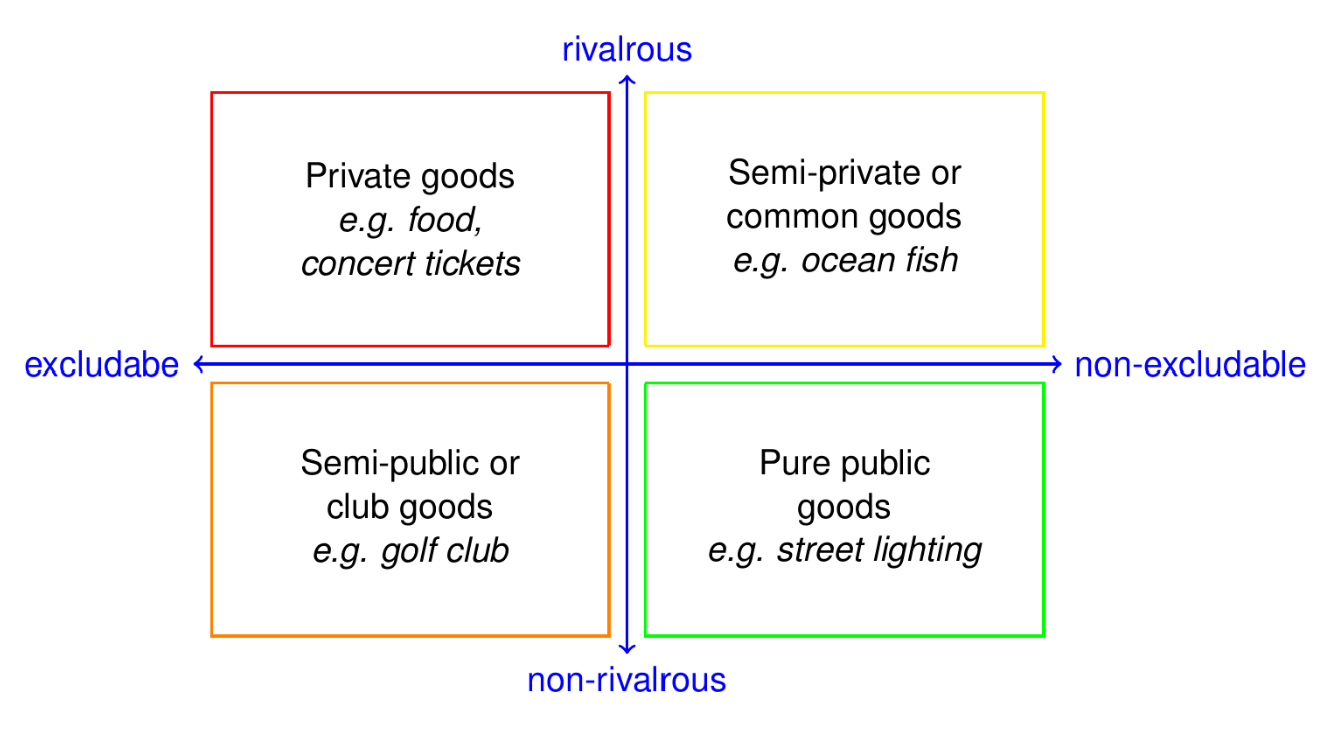
\includegraphics[width = \textwidth]{./img/figure14.png}
  \caption{Continuous scale.}
\end{figure}
\subsection{Public goods in free markets}
\begin{figure}[H]
  \centering
  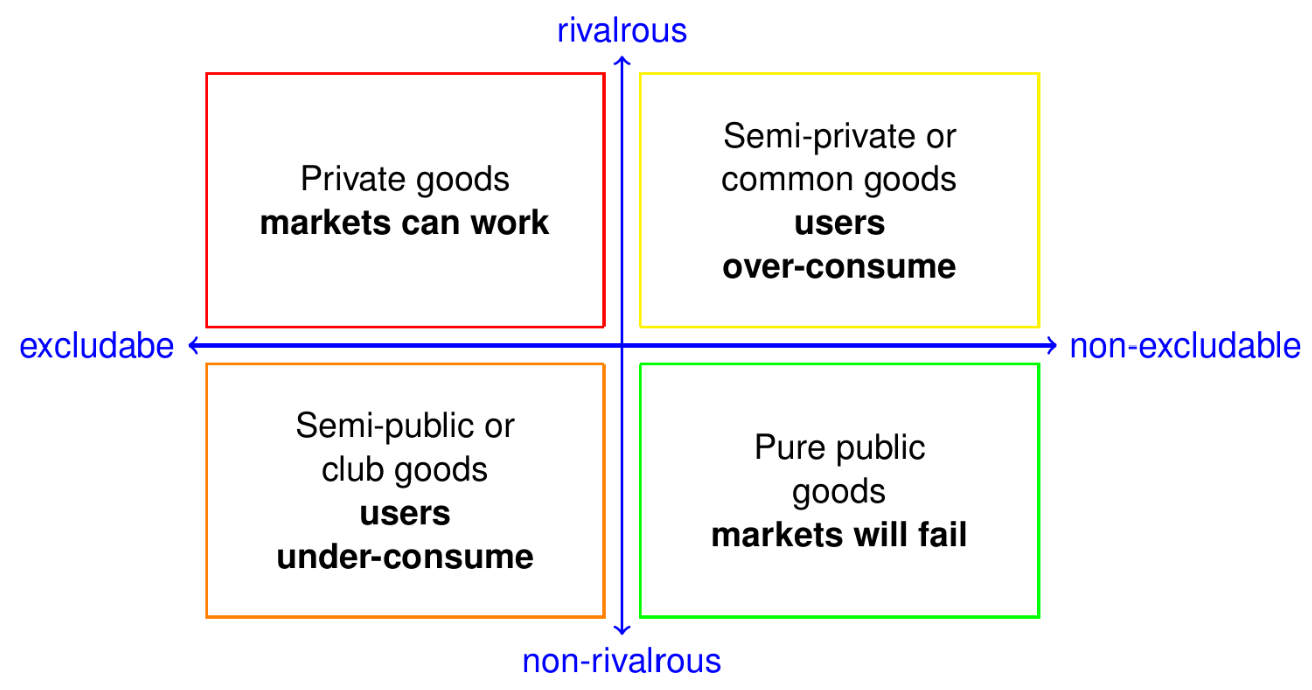
\includegraphics[width = \textwidth]{./img/figure15.png}
  \caption{Public goods in free markets.}
\end{figure}
\subsection{Public goods and market failure}
Pure public goods are \textbf{non-excludable}
\begin{itemize}
  \item Producers cannot exclude agents from consumption
  \item Unable to charge and therefore make profit
  \item Therefore (in theory) would not be produced through market action!
\end{itemize}
Possibility of funding via private cooperative, but\dots

\textbf{Free rider problem}
\begin{quote}
  as size of cooperative increases, possibility of avoiding contributing increases
\end{quote}
\subsubsection{Public sector provision}
Large group public goods supplied from public sector budget
\begin{itemize}
  \item Allocative role of government
\end{itemize}
\subsection{Privatisation in the public sector}
Note\dots Public sector provision $\neq$ equivalent public sector production.
\begin{quote}
  The creation of markets in public services has been one of the great defining shifts in the way government has been run over the past 30 years (Gash and Roos 2012)
\end{quote}
\section{Externalities}
\subsection{Positive and negative externalities}
Externalities
\begin{quote}
  when the actions of one economic agent directly affect other agent(s) outside the market mechanism (production/consumption)
\end{quote}
Externalities can arise from either production or consumption and have a net positive or negative effect.
\subsection{Negative production externality}
\begin{figure}[H]
  \centering
  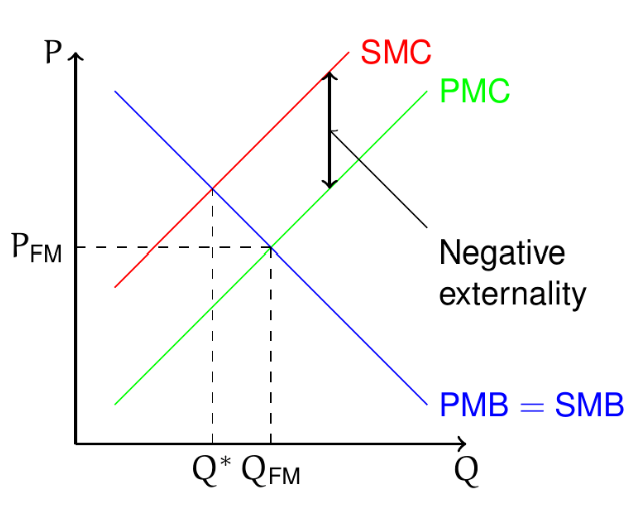
\includegraphics[width = 0.5\textwidth]{./img/figure16.png}
  \caption{Negative production externality.}
\end{figure}
Production of output reduces well-being of third parties not involved in transaction,
\begin{itemize}
  \item e.g. oil spills during fuel production pollute oceans and damage wildlife
  \item leads to overproduction
\end{itemize}
\subsection{Negative consumption externality}
\begin{figure}[H]
  \centering
  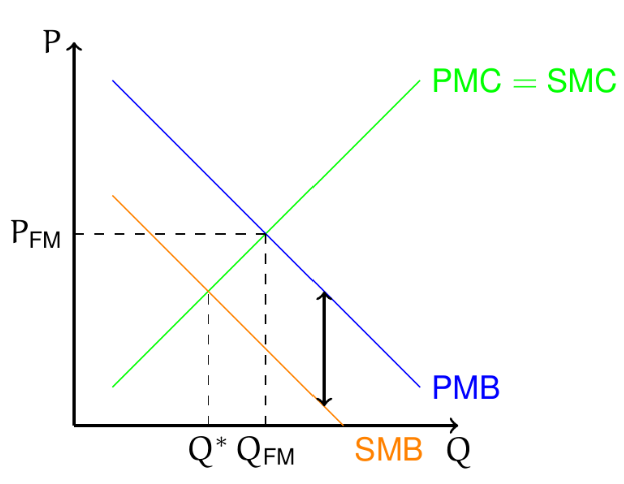
\includegraphics[width = 0.5\textwidth]{./img/figure17.png}
  \caption{Negative consumption externality.}
\end{figure}
Consumption of output reduces well-being of third parties not involved in transaction,
\begin{itemize}
  \item e.g. driving cars produces carbon emissions
  \item leads to overconsumption
\end{itemize}
\subsection{Positive production externality}
\begin{figure}[H]
  \centering
  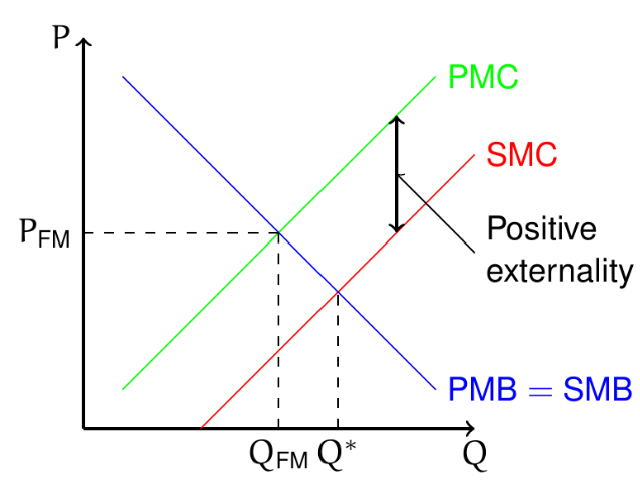
\includegraphics[width = 0.5\textwidth]{./img/figure18.png}
  \caption{Positive production externality.}
\end{figure}
Production of output reduces well-being of third parties not involved in transaction,
\begin{itemize}
  \item e.g. creating a new tourist attraction brings increases custom to local shops
  \item leads to underproduction
\end{itemize}
\subsection{Positive consumption externality}
\begin{figure}[H]
  \centering
  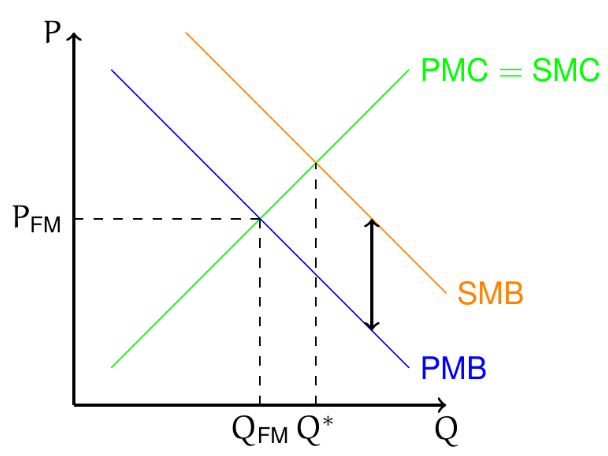
\includegraphics[width = 0.5\textwidth]{./img/figure19.png}
  \caption{Positive consumption externality.}
\end{figure}
Consumption of output reduces well-being of third parties not involved in transaction,
\begin{itemize}
  \item e.g. cycling improves peoples general health, reducing pressure on public healthcare
  \item leads to under-consumption
\end{itemize}
\subsection{Externalities and property rights}
Externalities can be transferred where third party benefit/cost is clear i.e. where property rights are well defined.
\subsection{Managing externalities}
Where property rights are not clear, managing externalities relies on allocative role of government
\subsubsection{Public sector interventions}
Negative externalities:
\begin{itemize}
  \item Corrective taxes
  \item Quantity restrictions
  \item Standards
\end{itemize}
Positive externalities
\begin{itemize}
  \item Subsidies
  \item Tax benefits
  \item Direct production
\end{itemize}
\subsection{Externalities and the environment}
Note\dots Externalities related to climate change are critical to long term sustainability of the planet.
\subsubsection{COP26}
\begin{quote}
  ``Climate change is the single benefit health treat facing humanity. While no one is safe from the health impacts of climate change, they are disproportionality felt by the most vulnerable and disadvantaged.'' (World Health Organisation 2021)
\end{quote}
\subsection{The doughnut economic model}
\begin{figure}[H]
  \centering
  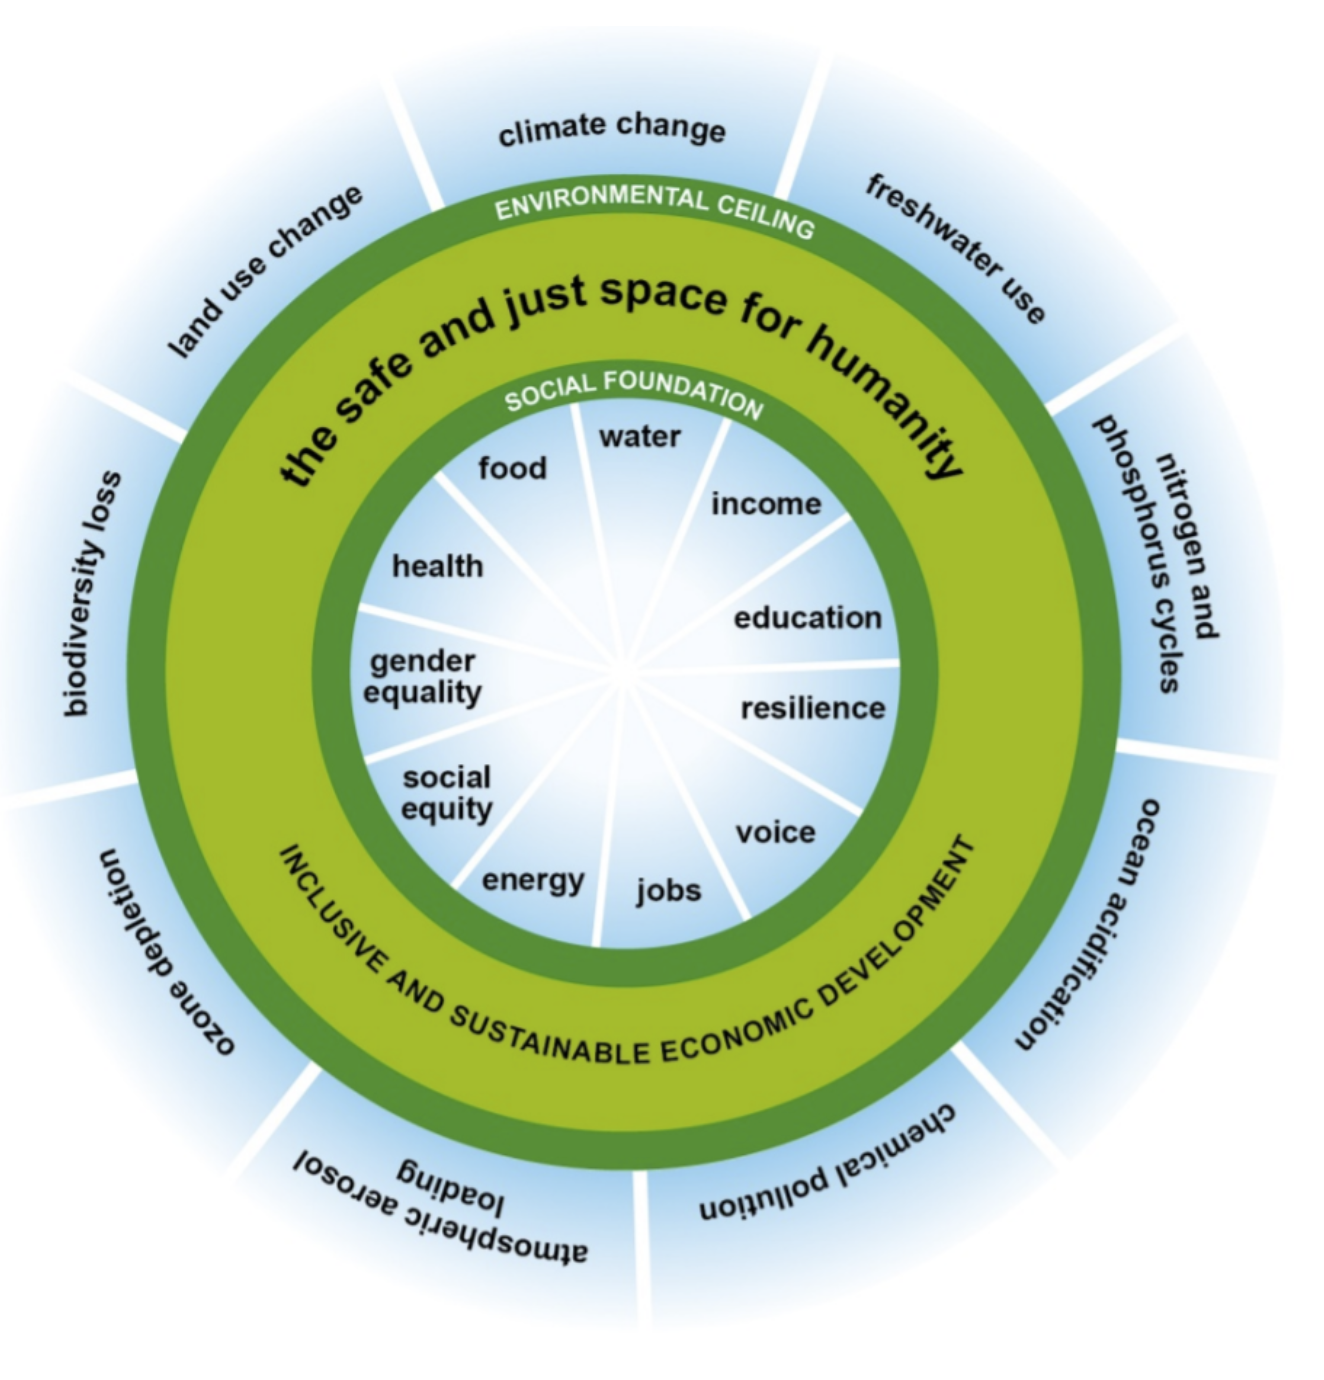
\includegraphics[width = \textwidth]{./img/figure20.png}
  \caption{Doughnut economic model.}
\end{figure}
\chapter{Techniques for Project Evaluation}
\section{Introduction to Capital and Interest}
\subsection{Capital}
\begin{itemize}
  \item \textbf{Capital} is wealth in the form of money or property that can be used to produce more wealth
  \item A pound is worth more than a pound one or two years from now because of the \textbf{interest} it can earn
  \item Therefore money has a \textbf{time value}
  \item Often the riskiest thing a person can do with money is nothing
\end{itemize}
\subsection{Interest}
\begin{itemize}
  \item Interest pays the providers of capital for:
        \begin{itemize}
          \item Forgoing its use during the time the capital is being used
          \item The risk the investor takes in permitting another person or organisation to use their capital
        \end{itemize}
  \item Investors must decide whether the return on their capital is sufficient to buy into a proposed project or venture
  \item The interest available from an alternative investment is the opportunity cost of using capital in the proposed undertaking
\end{itemize}
\section{Simple interest}
Interest earned or charged that is linearly proportional to the initial amount of the loan (principal), the interest rate, and the number of interest periods for which the principal is committed. Simple interest is not used frequently in modern commercial practice.
\begin{gather}
  I = PNi
\end{gather}
where:
\begin{itemize}
  \item $I$ is total simple interest
  \item $P$ is principal amount lent or borrowed
  \item $N$ is number of interest periods
  \item $i$ is interest rate per interest period
\end{itemize}
The total amount repaid at the end of $N$ interest periods is $P+I$. If \pounds 1000 were loaned for three years at a simple interest rate of 10\% per year, the interest earned would be \pounds 300. The total amount owed at the end of three years would be \pounds 1300.
\section{Compound interest}
Interest earned or charged that is based on the remaining principal amount plus any accumulated interest charges up to the beginning of that period. Compound interest considers the time value of money, and is much more common than simple interest.
\begin{gather}
  I = P\left(1 + i\right)^N - P
\end{gather}
The total amount repaid at the end of $N$ interest periods is $P+I$. If \pounds 1000 were loaned for three years at a compound interest rate of 10\% per year, the interest earned would be \pounds 331. The total amount owed at the end of three years would be \pounds 1331.
\subsection{Compound vs simple interest}
Assume that \pounds 1000 were loaned for three years at an interest rate of 10\% per year.
\begin{figure}[H]
  \centering
  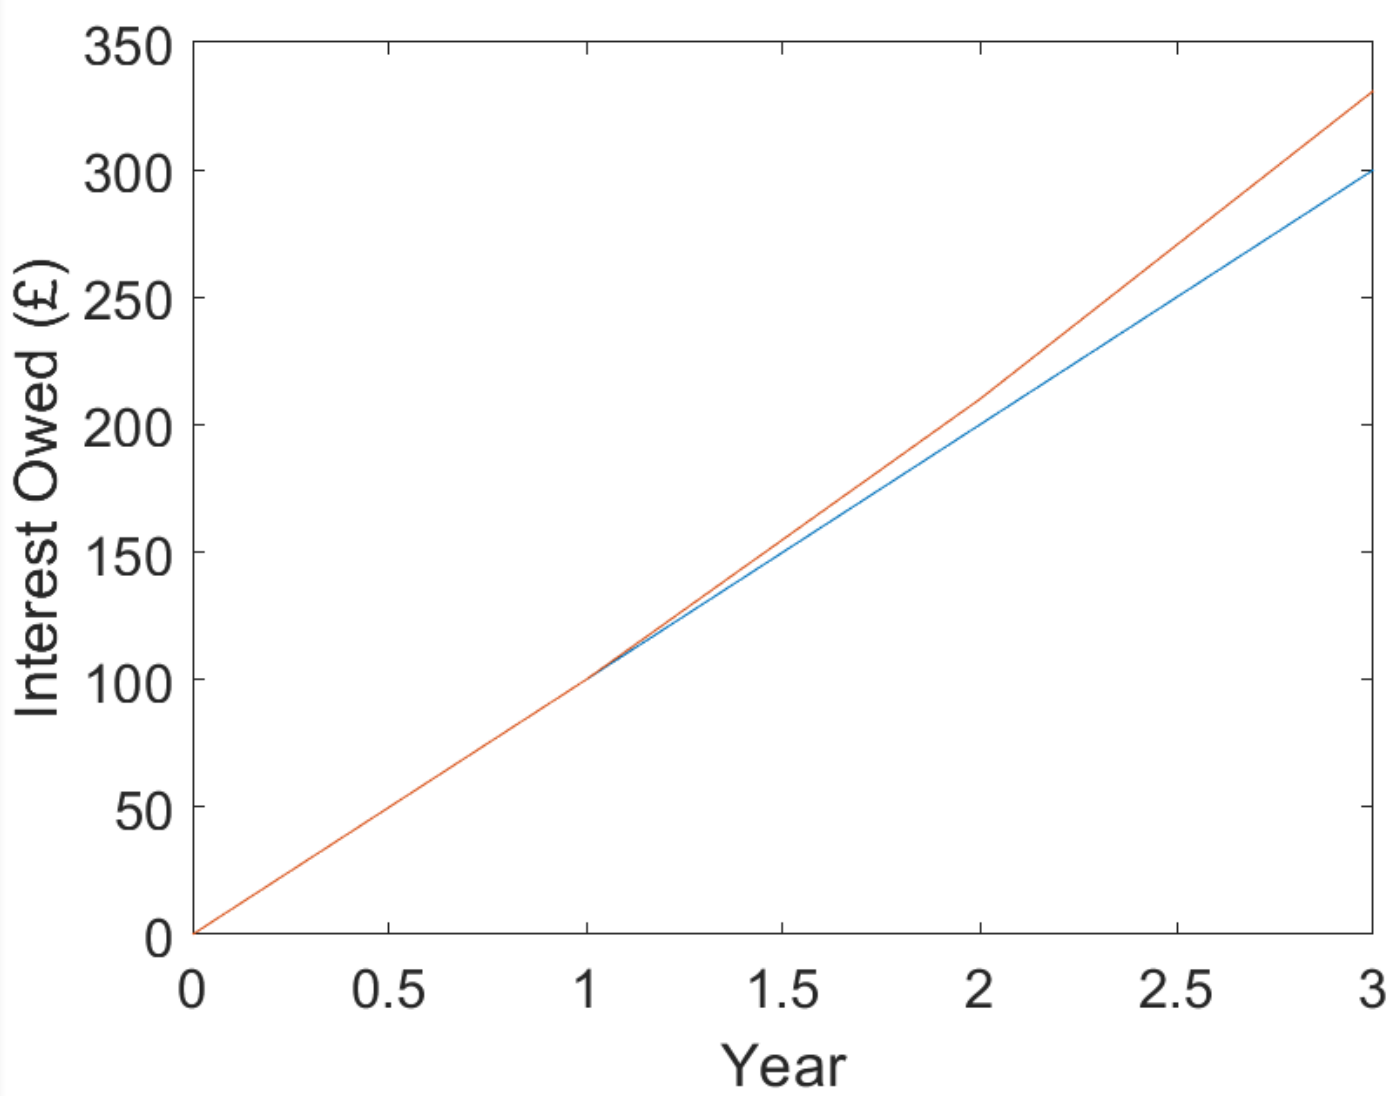
\includegraphics[width = 0.8\textwidth]{./img/figure21.png}
  \caption{Blue: simple interest, Orange: compound interest}
\end{figure}
\section{What is project evaluation}
\begin{itemize}
  \item Project evaluation considers the return that a given project will or should produce
  \item Project evaluation involves quantifying project profitability using various methods
  \item We address whether a proposed capital investment and its associated expenditures can be recovered by revenue (or savings) over a period of time, in addition to a return on the capital that is sufficiently attractive
\end{itemize}
\section{Minimum attractive rate of return (MARR)}
MARR is the \textbf{minimum rate of return} on a project that the top management of an organisation is willing to accept before starting a project. MARR depends on numerous factors:
\begin{itemize}
  \item Amount of money available for investment (as well as the source and costs of funds)
  \item The number of projects available for investment and their purpose (i.e. whether they are essential or optional)
  \item The amount of perceived risk and the estimated cost of administering projects over different planning horizons
  \item The type of organisation involved (government, public utility, private industry)
\end{itemize}
\section{Project evaluation using Net Present Value}
\subsection{Net present value (NPV)}
The NPV method examines the equivalent worth of all cash flows relative to some base point in time i.e. the present. The future value ($FV$) of a sum of money has a value today called the present value ($PV$), which depends on the interest rate / that can be obtained (generally the MARR) - note that we are talking about a single sum of money in this case. The $PV$ of a cashflow in $n$ years' time as a function of $i$ is:
\begin{gather}
  PV = \frac{FV}{\left(1 + i\right)^n}
\end{gather}
Note that $i$ is expressed as a decimal here. A series of uniform (annual) receipts ($AV$) have a value today called the present value ($PV$) which depends on the interest rate / that can be obtained (generally the MARR) - note that we are talking about multiple sums of money in this case. The $PV$ of a series of cashflows that occur at the end of periods (years) 1 to $n$ is:
\begin{gather}
  PV = AV \frac{\left(1+i\right)^n -1}{i\left(1+i\right)^n} = \sum^n_{k=1}\frac{AV}{\left(1+i\right)^k}
\end{gather}
$NPV$ then accounts for all cash inflows and outflows:
\begin{gather}
  NPV = PV_{\textrm{cash inflows}} - PV_{\textrm{cash  outflows}}
\end{gather}
To use the NPV method to determine project worthiness, we compute $NPV$ using the MARR as the interest rate. The higher the interest rate ($i$) and the farther into the future a cash flow occurs, the lower its $PV$.
\begin{figure}[H]
  \centering
  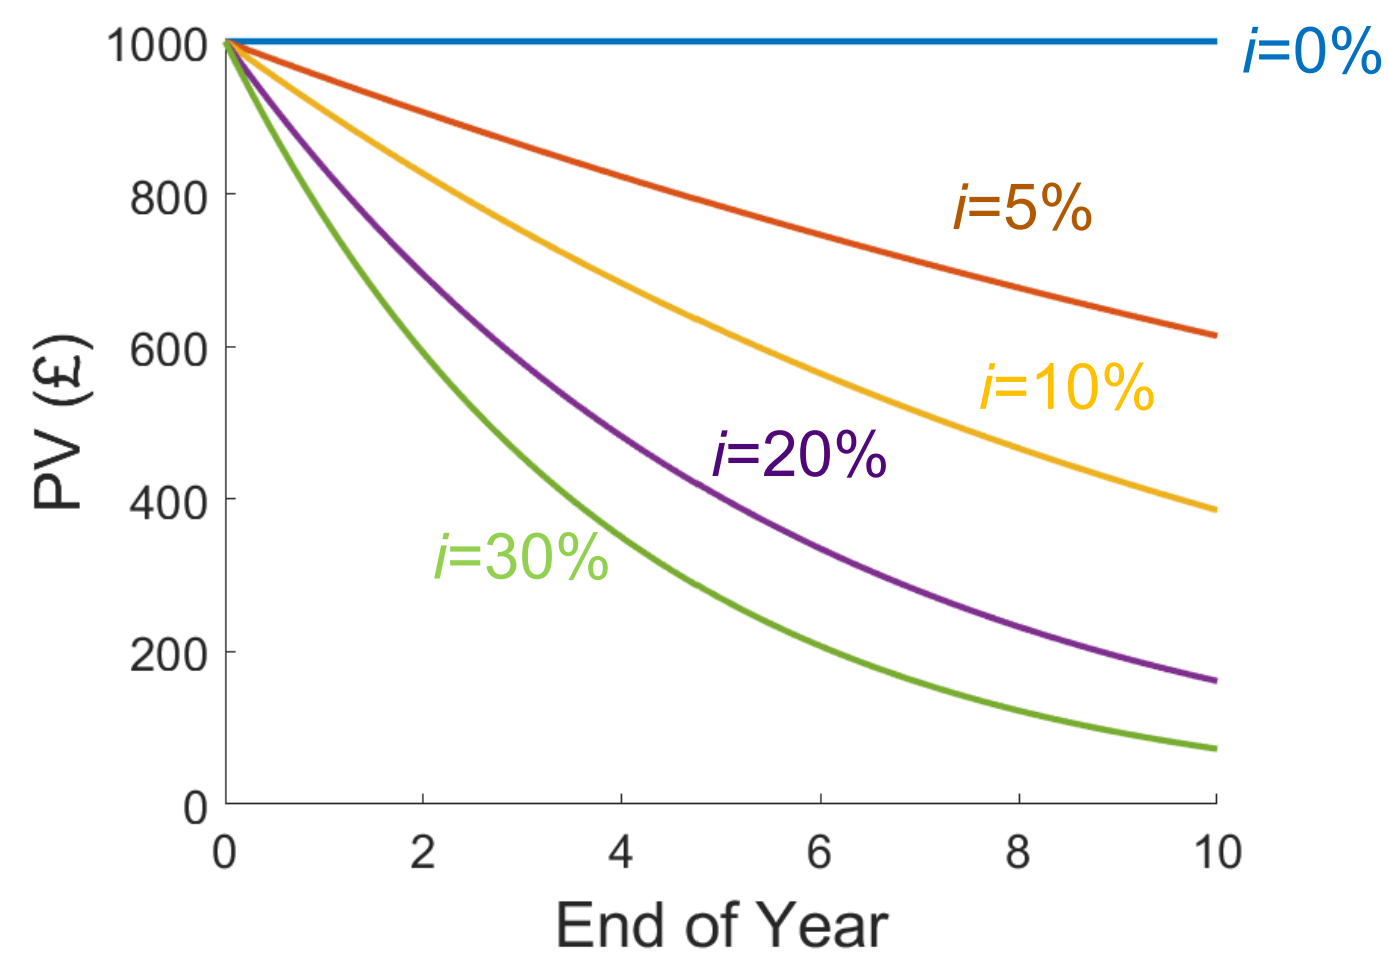
\includegraphics[width = 0.8\textwidth]{./img/figure22.png}
  \caption{Effect of interest rate on PV.}
\end{figure}
\subsection{Example}
A retrofitted heat-pump system is being considered for a small office building. The system can be installed and purchased for \pounds 110,000 and it will save an estimated 300,000 kilowatt-hours of electric power each year over a six-year period. A kilowatt-hour of electricity costs \pounds 0.10, and the company uses a MARR of 15\% per year in its economic evaluations of refurbished systems. The market value of the system will be \pounds 8,000 at the end of six years, and additional annual operating and maintenance expenses are negligible. Use the NPV method to determine whether the system should be installed.
\begin{gather}
  NPV = PV\textrm{ of estimated savings} + PV\textrm{ of market value} -PV\textrm{ of cost}
\end{gather}
Estimated value:
\begin{gather}
  PV_{ES} = 300000\times 0.1 = 30000\\
  PV_{ES,y1} = \frac{30000}{(1+0.15)^1}\\
  PV_{ES,y2} = \frac{30000}{(1+0.15)^2}\dots\\
  PV_{ES,y6} = \frac{30000}{(1+0.15)^6} \\
  \therefore\sum_{k=1}^6\frac{30000}{(1+0.15)^k}
\end{gather}
Market value:
\begin{gather}
  PV_{MV} = \frac{8000}{(1+0.15)^6}
\end{gather}
Cost:
\begin{gather}
  PV_{cost} = 110000
\end{gather}
Therefore, NPV is:
\begin{gather}
  NPV = \sum_{k=1}^6\frac{30000}{(1+0.15)^k} +\frac{8000}{(1+0.15)^6} - 110000 \approx 6993
\end{gather}
\subsection{Advantages and disadvantages of NPV}
Advantages
\begin{itemize}
  \item It accounts for the time value of money
  \item It accounts for uncertainties about future projections
  \item It accounts for all cash flows of interest
\end{itemize}
Disadvantages
\begin{itemize}
  \item It is highly sensitive to the interest rate used
  \item It is not useful for comparing projects of different sizes
  \item It ignores costs that are incurred before the project starts
\end{itemize}
\section{Project evaluation using Internal Rate of Return}
\subsection{Internal Rate of Return (IRR)}
The IRR method solves for the interest rate that equates the present value of cash inflows (receipts or savings) to the present value of cash outflows (expenditures, e.g. investment costs). That is, the IRR provides the answer to the question: what interest rate provides an NPV of 0? This method is the most widely using rate-of-return method for performing engineering economic analyses.
\begin{figure}[H]
  \centering
  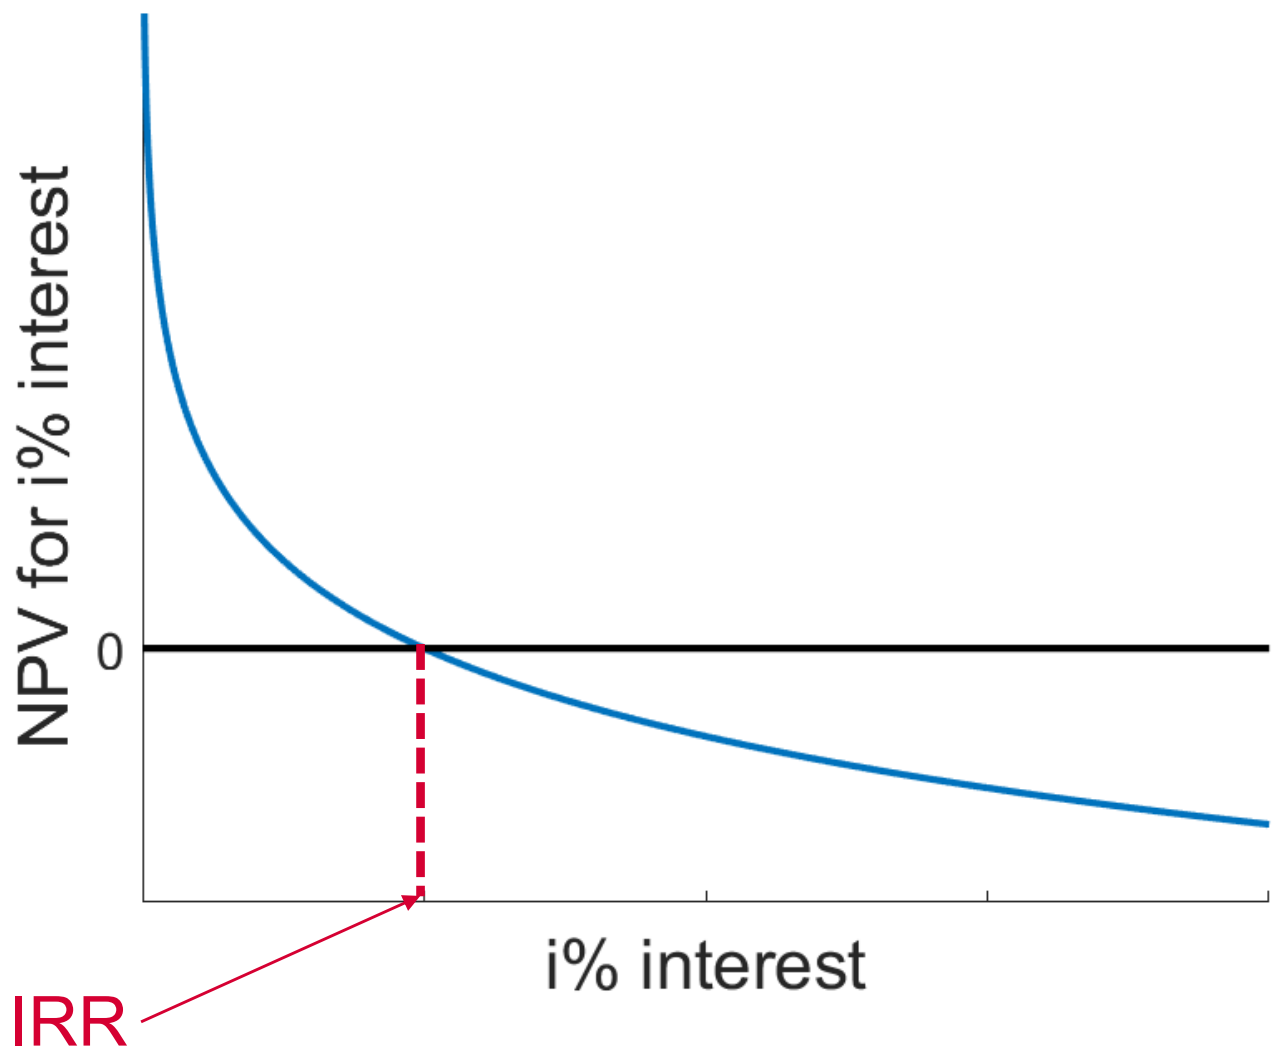
\includegraphics[width = 0.7\textwidth]{./img/figure23.png}
  \caption{Internal Rate of Return.}
\end{figure}
\subsection{Example}
A company is considering the purchase of a digital camera for the maintenance of design specifications by feeding digital pictures directly into an engineering workstation where computer-aided design files can be superimposed over the digital pictures. Differences between the two images can be noted, and corrections as appropriate can then be made by design engineers. The capital investment requirement is \pounds 345,000 and the estimated market value of the system after a six-year study period is \pounds 115,000. Annual revenues attributable to the new system will be \pounds 120,000 and additional annual expenses will be \pounds 22,000. You have been asked by management to determine the IRR of this project and to make a recommendation. The corporation's MARR is 20\% per year.

Denote IRR as $i$. First let's determine an equation for NPV:
\begin{gather}
  NPV = PV \textrm{ of net annual revenue} + PV \textrm{ of market value} - PV \textrm{ of cost}
\end{gather}
PV of net annual revenue:
\begin{gather}
  PV_{NAR,y1} = \frac{120000-22000}{(1+i)^1}\\
  PV_{NAR,y2} = \frac{120000-22000}{(1+i)^2}\dots\\
  PV_{NAR,y6} = \frac{120000-22000}{(1+i)^6}\\
  \therefore \sum_{k=1}^6 \frac{98000}{(1+i)^k}
\end{gather}
Market Value:
\begin{gather}
  PV_{MV} = \frac{115000}{(1+i)^6}
\end{gather}
Cost:
\begin{gather}
  PV_{cost} = 345000
\end{gather}
NPV:
\begin{gather}
  NPV = \sum_{k=1}^6 \frac{98000}{(1+i)^k} + \frac{115000}{(1+i)^6} - 345000
\end{gather}
Lets try $i = MARR = 20\% = 0.2$:
\begin{gather}
  NPV(i=0.2) = + 19,413
\end{gather}
However, this is not the IRR\dots We must calculate $i$ using a solver to find which value of $i$ gives and NPV of 0. Using Excel, we find that our IRR is 22\%. Interpolation may also be used.
\subsection{Advantages and disadvantages of IRR}
Advantages:
\begin{itemize}
  \item It has widespread acceptance in industry
  \item It is relatively simple to understand
  \item It accounts for the time value of money
\end{itemize}
Disadvantages
\begin{itemize}
  \item It is difficult to compute
  \item It ignores the size and scope of projects
  \item It does not account for the actual reinvestment rate
\end{itemize}
\section{Project evaluation using Payback Period}
The payback period method evaluates the number of years $\Theta$ it takes for cash inflows to equal cash outflows. Both of the previous evaluation methods focus on profitability. The payback period instead estimates a company's liquidity (i.e. how fast an investment can be recovered). There are two types of payback period methods:
\begin{enumerate}
  \item Simple payback period - ignores the time value of money
  \item Discounted payback period - accounts for the time value of money
\end{enumerate}
\subsection{Simple Payback Period Example}
A public school is being renovated for \pounds 13.5 million. The building has geothermal heating and cooling, high-efficiency windows, and a solar array that permits the school to sell electricity back to the local electric utility. The annual value of these benefits is estimated to be \pounds 2.7 million. In addition, the residual value of the school at the end of its 40-year life is negligible. What is the simple payback period for the renovated school?

The simple payback period is:
\begin{gather}
  SPP = \frac{13.5}{2.7} = 5 \textrm{ years}
\end{gather}
\subsection{Simple \& Discounted Payback Period Example}
A piece of new equipment has been proposed by engineers to increase the productivity of a certain manual welding operation. The investment cost is \pounds 25,000 and the equipment will have a market value of \pounds 5,000 at the end of its expected life of 5 years. Increased productivity attributable to the equipment will amount to \pounds 8,000 per year after extra operating costs have been subtracted from the value of the additional production. MARR is 20\% per year. Calculate the simple and the discounted payback periods.
\begin{figure}[H]
  \centering
  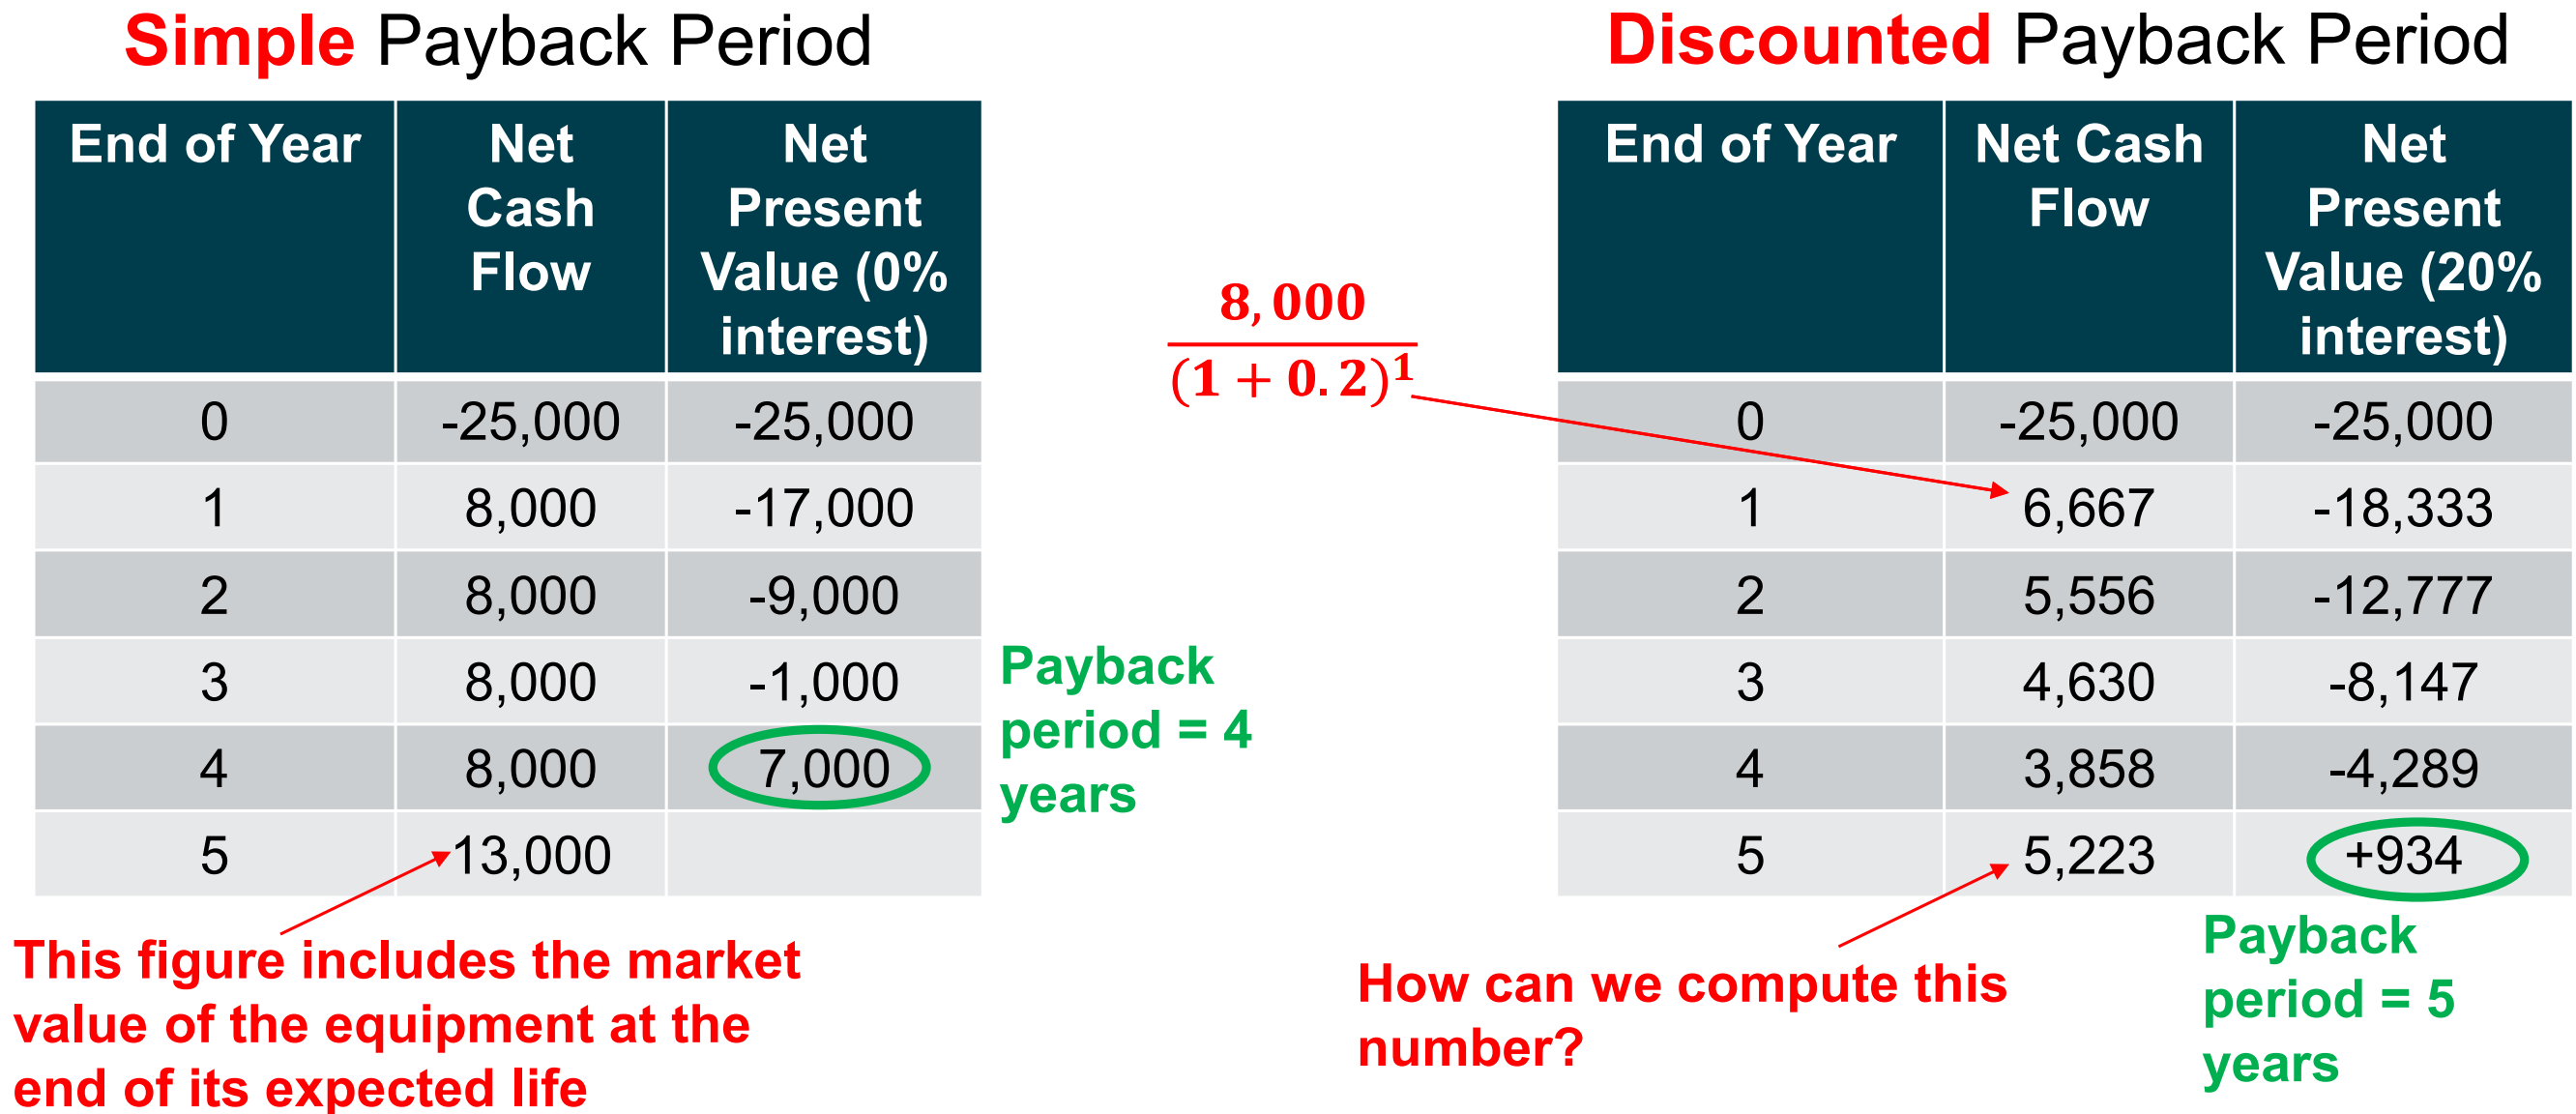
\includegraphics[width = \textwidth]{./img/figure24.png}
  \caption{Simple and discounted payback periods.}
\end{figure}
\subsection{Advantages and disadvantages of payback period}
Advantages
\begin{itemize}
  \item It provides a new perspective on performance (by focusing on liquidity)
  \item It is relatively simple to understand and compute
  \item It requires relatively few inputs
\end{itemize}
Disadvantages
\begin{itemize}
  \item It does not account for cash flows that occur after the payback period
  \item It may not consider the time value of money
  \item It ignores profitability, and should only be used as a secondary evaluation measure.
\end{itemize}
\chapter{Cost-Benefit Analysis}
\section{What is cost-benefit analysis?}
\begin{quote}
  ``Assessing costs and benefits across all affected groups or places matters because even a proposal with a relatively low public sector cost such as new regulation, may have significant effects on specific groups in society, places or business''
\end{quote}
\begin{itemize}
  \item A cost-benefit analysis is the process used to measure the benefits of a decision or taking action relative to the associated costs
  \item If benefits $>$ costs, the decision or action is a good one to take
  \item If costs $>$ benefits, the proposed action or decision should be reconsidered
  \item Cost benefit analysis can also be used to compare alternate decisions or actions
\end{itemize}
Both costs and benefits are required to be expressed in monetary terms, accounting for the time value of money. Costs may be categorised as:
\begin{itemize}
  \item Direct - e.g. labour costs, manufacturing costs, material costs
  \item Indirect - e.g. utilities, rent
  \item Intangible - e.g. reduced productivity because of a new process
  \item Opportunity - lost benefits (opportunities) when pursuing one strategy over another
\end{itemize}
Benefits may be categorised as:
\begin{itemize}
  \item Direct - e.g. increased revenue and sales
  \item Indirect - e.g. increased consumer interest
  \item Intangible - e.g. improved employee morale
  \item Competitive - e.g. being an industry leader
\end{itemize}
\section{The Benefit-Cost Ratio method}
The Benefit-Cost Ratio (BCR) is defined as the ratio of the equivalent value of benefits to the equivalent value of costs. The equivalent-value measure can be:
\begin{itemize}
  \item Annual value (AV)
  \item Present value (PV)
  \item Future value (FV)
\end{itemize}
The BCR method has been the accepted procedure for making decisions and comparing projects in the public sector for many decades.
\begin{quote}
  if BCR $\geq$ 1, the project is acceptable
\end{quote}
Several different formulations of the BCR method have been developed. We examine two formulations of the BCR method that are commonly used by government agencies:
\begin{itemize}
  \item Conventional BCR method
  \item Modified BCR method
\end{itemize}
Both formulations will lead to identical project acceptability decisions (i.e. BCR $\geq$ 1 or BCR $<$ 1).
\subsection{Conventional BCR method}
Present value (PV) formulation:
\begin{gather}
  BCR_{PV} = \dfrac{PV_{benefits}}{PV_{costs}}\\
  BCR_{PV} = \dfrac{PV_{benefits}}{I- PV_{MV}+PV_{O\&M}}
\end{gather}
Annual value (AV) formulation:
\begin{gather}
  BCR_{AV} = \dfrac{AV_{benefits}}{AV_{costs}}\\
  BCR_{AV} = \dfrac{AV_{benefits}}{CR + AV_{O\&M}}
\end{gather}
Both ratios lead to identical numerical results. Where:
\begin{itemize}
  \item $I$ is initial investment in the proposed project
  \item $MV$ is market value at the end of useful life
  \item $O\&M$ is operating and maintenance costs
  \item $CR$ is capital-recovery amount (i.e. equivalent cost of $I$, including an allowance for market or salvage value)
\end{itemize}
\subsection{Modified BCR method}
Present value (PV) formulation:
\begin{gather}
  BCR_{PV} = \dfrac{PV_{benefits}}{PV_{costs}}\\
  BCR_{PV} = \dfrac{PV_{benefits} - PV_{O\&M}}{I - PV_{MV}}
\end{gather}
Annual value (AV) formulation:
\begin{gather}
  BCR_{AV} = \dfrac{AV_{benefits}}{AV_{costs}}\\
  BCR_{AV} = \dfrac{AV_{benefits}-AV_{O\&M}}{CR}
\end{gather}
Both ratios lead to identical numerical results.
\subsection{Conventional and modified BCRs}
Remember the formula for PV:
\begin{gather}
  PV = \dfrac{FV}{(1+i)^n}
\end{gather}
Present value (PV) of a future value (FV) in $n$ years, for an interest rate $i$.
Remember the formula for AV:
\begin{gather}
  AV = PV\dfrac{i(1+i)^n}{(1+i)^n - 1}
\end{gather}
Value of a series of uniform (annual) receipts (AV) that occur at the end of periods (years) 1 to $n$, given their present value (PV) and an interest rate $i$.
\subsection{What value of i to use?}
There are three main considerations when it comes to what interest rate to use for engineering economy studies of public-sector projects:
\begin{itemize}
  \item the interest rate on borrowed capital
  \item The opportunity cost of capital to the government agency
  \item The opportunity cost of capital to the taxpayers
\end{itemize}
\subsection{Why do conventional and modified BCRs lead to the same decision?}
Conventional BCR formulation:
\begin{gather}
  BCR_V = \frac{V_{benefits}}{I - V_{MV}+V_{O\& M}} = \frac{B}{C}
\end{gather}
Where subscript $V$ denotes either PV or AV. Modified BCR formulation:
\begin{gather}
  BCR_V = \frac{V_{benefits} \textcolor{red}{-V_{O\&M}}}{I - V_{MV} + V_{O\&M} \textcolor{red}{-V_{O\&M}}} = \frac{B\textcolor{red}{-X}}{C\textcolor{red}{-X}}
\end{gather}
Both the numerator and denominator differ by the same constant.
\begin{gather}
  \textcolor{red}{\frac{B}{C>1}}\rightarrow B > C \rightarrow B - X > C - X \rightarrow \textcolor{red}{\frac{B-X}{C-X}>1}
\end{gather}
leading to the same decision.
\subsection{Example 1}
The Greater London Authority is considering extending the runways of Stansted Airport so that larger commercial airplanes can use the facility. The land necessary for the runway extension is currently a farmland that can be purchased for \pounds 350,000. Construction costs for the runway extension are projected to be \pounds 600,000, and the additional annual maintenance costs for the extension are estimated to be \pounds 22,500. If the runways are extended, a small terminal will be constructed at a cost of \pounds 250,000. The annual operating and maintenance costs for the terminal are estimated at \pounds 75,000. Finally, the projected increase in flights will require the addition of two air traffic controllers at an annual cost of \pounds 100,000. Annual benefits of the runway extension have been estimated as follows:
\begin{table}
  \centering
  \begin{tabular}{@{}ll@{}}
    \toprule
    \textbf{Description}                            & \textbf{Annual benefit}  \\
    \midrule
    Leasing fee receipts from airlines              & \pounds 325,000          \\
    Passenger airport tax receipts                  & \pounds 65,000           \\
    Convenience benefit for residents near Stansted & \pounds 50,000           \\
    Additional tourism money for London             & \pounds 50,000           \\
    \midrule
    \textbf{Total}                                  & \textbf{\pounds 490,000} \\
    \bottomrule
  \end{tabular}
  \caption{Example 1.}
\end{table}
Apply the BCR method with a study of 20 years and a MARR of 10\% per year to determine whether the runways at Stansted airport should be extended.

Information provided:
\begin{gather}
  i = 0.1\\
  n = 20\, \textrm{years}\\
  I = \pounds 350000 + \pounds 600000 + \pounds 250000 = \pounds 1200000\\
  AV_{benefits} = \pounds 490000\\
  PV_{MV} = AV_{MV} = \pounds 0\\
  AV_{O\&M} = \pounds 22500 + \pounds 75000 + \pounds 100000 = \pounds 197500
\end{gather}
First, we need to determine PVs and AVs using:
\begin{gather}
  PV = AV\frac{\left(1+i\right)^n - 1}{i\left(1 + i\right)^n}\\
  AV = PV\frac{i\left(1+i\right)^n}{\left(1+i\right)^n - 1}
\end{gather}
\begin{gather}
  PV_{benefits} = \pounds 4171646\\
  PV_{O\&M} = \pounds 1681429\\
  AV_I = CR = \pounds 140951
\end{gather}
Conventional BCRs:
\begin{gather}
  BCR_{PV} = \frac{PV_{benefits}}{I - PV_{MV}+PV_{O\&M}} = 1.448\\
  BCR_{AV} = \frac{AV_{benefits}}{CR + AV_{O\&M}} = 1.448
\end{gather}
Modified BCRs:
\begin{gather}
  BCR_{PV} = \frac{PV_{benefits} - PV_{O\&M}}{I - PV_{O\&M}} = 2.075\\
  BCR_{AV} = \frac{AV_{benefits}- AV_{O\&M}}{CR} = 2.075
\end{gather}
BCR $\geq$ 1 in all cases, so runway should be extended.
\subsection{Issues of concern using BCRs}
\begin{itemize}
  \item The treatment of disbenefits
        \begin{itemize}
          \item Negative consequences to the public resulting from the implementation of a public sector project
        \end{itemize}
  \item The treatment of certain cash flows as additional benefits or reduced costs
\end{itemize}
\subsection{Treatment of disbenefits}
Disbenefits can be incorporated in BCR calculations by:
\begin{itemize}
  \item Reducing benefits accordingly (traditional approach) or
  \item Increasing costs accordingly
\end{itemize}
How do these approaches affect the BCR? How do these approaches affect the final decision?
\subsection{Example 2}
Refer back to Example 1. Suppose that there are disbenefits associated with the runway extension project. Specifically, the increased noise level from commercial jet traffic will be a serious nuisance to homeowners living along the approach path Stansted Airport. The annual disbenefit to these citizens is estimated to be \pounds 100,000.

Reapply the conventional BCR method, with equivalent annual worth, to determine whether this disbenefit affects your recommendation on the desirability of this project.

Disbenefit treated as a reduced benefit:
\begin{gather}
  BCR_{AV} = \frac{AV_{benefits}-100000}{CR + AV_{O\&M}} = 1.152
\end{gather}
Disbenefit treated as an increased cost:
\begin{gather}
  BCR_{AV} = \frac{AV_{benefits}}{CR + AV_{O\&M}+100000} = 1.118
\end{gather}
BCR $\geq$ 1 in both cases, so runway should be extended. The treatment of disbenefits affects the magnitude of the BCR, but not the decision.
\subsection{Treatment of certain cash flows}
Certain cash flows can be incorporated in BCR calculations by:
\begin{enumerate}
  \item Increasing benefits accordingly
  \item Reducing costs accordingly
\end{enumerate}
How do these approaches affect the BCR? How do these approaches affect the final decision?
\subsection{Example 3}
Transport for London is considering upgrading an ageing bridge across the Thames. The existing two-lane bridge is expensive to maintain and creates a traffic bottleneck because the road is four lanes wide on either side of the bridge. The new bridge can be constructed at a cost of \pounds 300,000, and estimated annual maintenance costs are \pounds 10,000. The existing bridge has annual maintenance costs of \pounds 18,500. The annual benefit of the new four-lane bridge to motorists, due to the removal of the traffic bottleneck, has been estimated to be \pounds 25,000.

Conduct a cost-benefit analysis based on equivalent annual worth, using a MARR of 8\% and a study period of 25 years, to determine whether the new bridge should be constructed.

Information provided:
\begin{gather}
  i = 0.08\\
  n = 25\, \textrm{years}\\
  I = \pounds 300000\\
  AV_{benefits} = \pounds 25000\\
  PV_{MV} = AV_{MV} = \pounds 0\\
  AV_{O\&M} = \pounds 10000 - \pounds 18500 = \textcolor{red}{-\pounds 8500}
\end{gather}
Cost is negative because it represents a reduction with respect to the current cost.

Required information:
\begin{gather}
  AV_I = CR = \pounds 28104
\end{gather}
Reduced cost treated as a reduced cost (conventional BCR approach):
\begin{gather}
  BCR_{AV} = \frac{BCR_{AV}}{CR + AV_{O\&M}} = 1.275
\end{gather}
Reduced cost treated as an increased benefit (modified BCR approach):
\begin{gather}
  BCR_{AV} = \frac{AV_{benefits} - AV_{O\&M}}{CR} = 1.192
\end{gather}
BCR $\geq$ 1 in both cases, so bridge should be constructed. The classification of the cash-flow items affects the magnitude of the BCR, but not the decision.
\subsection{Treatment of disbenefits/certain cash flows}
Arbitrary decisions on the classification of benefits and costs has no bearing on project acceptability because if X is classified as an added benefit:
\begin{gather}
  BCR = \frac{B \textcolor{red}{+ X }}{C}
\end{gather}
and
\begin{gather}
  BCR > 1 \rightarrow B + X > C \rightarrow B > C - X \rightarrow \frac{B}{C \textcolor{red}{- X}} > 1
\end{gather}
leading to the same decision.
\section{Evaluating independent projects using the BCR method}
\subsection{What are independent projects?}
Independent projects are categorised as groupings of projects for which the choice to select any particular project in the group is \textbf{independent} of choices regarding all other projects within the group.

It is therefore acceptable to select:
\begin{enumerate}
  \item None of the projects
  \item A combination of the projects
  \item All of the projects
\end{enumerate}
Formal comparisons of independent projects is unnecessary. The only criterion for selecting each independent project is BCR $\geq$ 1.
\subsection{Example 4}
Uncontrolled water flow has increased flow conditions along a river. You have independent options to alleviate the problem of building a reservoir and/or improving the channel. Relevant information is as follows:
\begin{table}[H]
  \centering
  \begin{tabular}{@{}lll@{}}
    \toprule
                     & Reservoir construction & Channel improvement \\
    \midrule
    $CR + AV_{O\&M}$ & \pounds 1,642,200      & \pounds 1,815,100   \\
    $AV_{benefits}$  & \pounds 1,742,200      & \pounds 2,856,300   \\
    \bottomrule
  \end{tabular}
  \caption{Example 4 information.}
\end{table}
Conduct a cost-benefit analysis using the conventional BCR method and equivalent annual worth to determine the best course of action.

Reservoir construction:
\begin{gather}
  BCR_{AV} = \frac{AV_{benefits}}{CR + AV_{O\&M}} = 1.061
\end{gather}
Channel improvement:
\begin{gather}
  BCR_{AV} = \frac{AV_{benefits}}{CR + AV_{O\&M}} = 1.574
\end{gather}
BCR $\geq$ 1 in both cases, so both options should be pursued (the fact that the channel improvement has a higher BCR is irrelevant).
\section{Evaluating mutually exclusive projects using the BCR method}
\subsection{What are mutually exclusive projects}
Mutually exclusive projects are a group of projects from which, \textbf{at most, one project may be selected.} Each mutually exclusive project can be viewed as a feasible design alternative. Because the BCR method provides a ratio of benefits to costs rather than a direct measure of a project's profit potential, \textbf{selecting the project that maximises the BCR does not guarantee that the best project is selected.}
\subsection{Procedure for evaluating mutually exclusive projects}
\begin{enumerate}
  \item Calculate equivalent value (PV, AV or FV) of costs for each mutually exclusive project
  \item Rank-order mutually exclusive projects by increasing equivalent value of costs (note: the rank-order will be the same for all equivalent value types)
  \item Calculate the BCR for the project with the lowest equivalent cost ($BCR_L$)
        \begin{itemize}
          \item If $BCR_L \geq 1 \rightarrow$ baseline = project with the lowest equivalent cost
          \item Else $\rightarrow$ baseline = ``do-nothing''
        \end{itemize}
  \item Follow the flow chart in Figure \ref{fig:EMEFC}
\end{enumerate}
\begin{figure}[H]
  \centering
  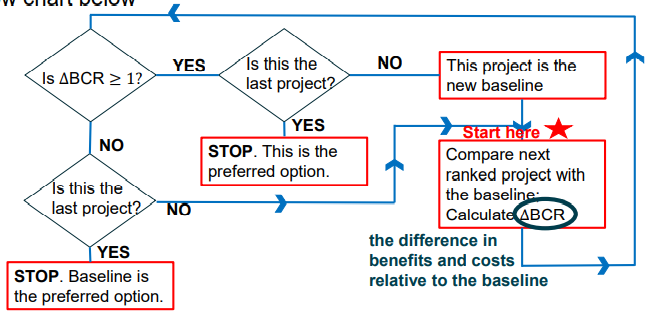
\includegraphics[width = 0.9\textwidth]{./img/figure25.png}
  \caption{Flow chart for evaluating mutually exclusive projects}
  \label{fig:EMEFC}
\end{figure}
\subsection{Example 5}
Three mutually exclusive public-works projects are currently under consideration. Their respective costs and benefits are included in the table that follows. Each of the projects has a useful life of 50 years, and MARR is 10\% per year.
\begin{table}[H]
  \centering
  \begin{tabular}{@{}llll@{}}
    \toprule
                       & Project A         & Project B          & Project C          \\
    \midrule
    Capital investment & \pounds 8,500,000 & \pounds 10,000,000 & \pounds 12,000,000 \\
    Annual O\&M costs  & \pounds 750,000   & \pounds 725,000    & \pounds 700,000    \\
    Market value       & \pounds 1,250,000 & \pounds 1,750,000  & \pounds 2,000,000  \\
    Annual benefit     & \pounds 2,150,000 & \pounds 2,265,000  & \pounds 2,500,000  \\
    \bottomrule
  \end{tabular}
  \caption{Example 5 information.}
\end{table}
Which, if any of these projects, should be selected?

Information provided and required information:
\begin{gather}
  i = 0.1\\
  n = 50\, \textrm{years}
\end{gather}
Step 1: convert to PV.
\begin{table}[H]
  \centering
  \begin{tabular}{@{}llll@{}}
    \toprule
                    & Project A          & Project B          & Project C          \\
    \midrule
    I               & \pounds 8,500,000  & \pounds 10,000,000 & \pounds 12,000,000 \\
    $PV_{O\&M}$     & \pounds 7,436,111  & \pounds 7,188,241  & \pounds 6,940,370  \\
    $PV_{MV}$       & \pounds 10,648     & \pounds 14,907     & \pounds 17,037     \\
    $PV_{costs}$    & \pounds 15,925,463 & \pounds 17,173,333 & \pounds 18,923,333 \\
    $PV_{benefits}$ & \pounds 21,316,851 & \pounds 22,457,055 & \pounds 24,787,036 \\
    \bottomrule
  \end{tabular}
  \caption{Example 5 required information.}
\end{table}
Step 2
\begin{gather}
  BCR_A = \frac{21316851}{15925463} = 1.339 \geq 1 \rightarrow\, \textrm{Project A is the baseline}
\end{gather}
Step 3: establish baseline.

Step 4:
\begin{gather}
  \Delta BCR_{B} = \frac{22457055-21316851}{17173333-15925463} = 0.914 < 1 \rightarrow\, \textrm{Project A is still the baseline}
\end{gather}
Proceed to Project C
\begin{gather}
  \Delta BCR_{C} = \frac{24787036-21316851}{18923333-15925463} = 1.158 \geq 1 \rightarrow\, \textrm{Project C is the preferred option}
\end{gather}
\subsection{Mutually exclusive projects with unequal lives}
It is not uncommon for public projects to have different useful lives. How can we conduct BCR analyses in these cases? In these cases, annual values (AVs) should be used to conduct incremental cost-benefit analyses.
\subsection{Example 6}
Two mutually exclusive alternative public-works projects are under consideration. Their respective costs and benefits are included in the table that follows. Project A has an anticipated life of 35 years, and the useful life of Project B has been estimated to be 25 years. The effect of inflation is negligible.
\begin{table}[H]
  \centering
  \begin{tabular}{@{}lll@{}}
    \toprule
                       & Project A       & Project B       \\
    \midrule
    Capital investment & \pounds 750,000 & \pounds 625,000 \\
    Annual O\&M costs  & \pounds 120,000 & \pounds 110,000 \\
    Annual benefit     & \pounds 245,000 & \pounds 230,000 \\
    \bottomrule
  \end{tabular}
  \caption{Example 6 information.}
\end{table}
If the MARR is 9\% per year, which, if either, of these projects should be selected?

Information provided and required information:
\begin{gather}
  i = 0.09\\
  n = 35 \textrm{ or } 25\, \textrm{years}
\end{gather}
Step 1: convert to AV.
\begin{table}[H]
  \centering
  \begin{tabular}{@{}lll@{}}
    \toprule
                    & Project A       & Project B       \\
    \midrule
    $AV_I$          & \pounds 70,977  & \pounds 63,629  \\
    $AV_{O\&M}$     & \pounds 120,000 & \pounds 110,000 \\
    $AV_{MV}$       & \pounds 0       & \pounds 0       \\
    $AV_{costs}$    & \pounds 190,977 & \pounds 173,629 \\
    $AV_{benefits}$ & \pounds 245,000 & \pounds 230,000 \\
    \bottomrule
  \end{tabular}
  \caption{Example 6 required information.}
\end{table}
Step 2:
\begin{gather}
  BCR_B = \frac{230000}{173629} = 1.325 \geq 1 \rightarrow \, \textrm{Project B is the baseline}
\end{gather}
Step 3: establish baseline.

Step 4:
\begin{gather}
  \Delta BCR_A = \frac{245000 - 230000}{190977-173629}=0.865<1\rightarrow\,\textrm{Project B is the preferred option}
\end{gather}
\chapter{Companies and Financial Accounting}
\section{Companies}
\subsection{What is a company?}
A company is a legal entity (``personality'') that can issue contracts, enter into agreements or contracts, assume obligations, incur and pay debts, sue and be sued in its own right, and be held responsible for its own actions. There are three main types of companies in the UK:
\begin{enumerate}
    \item A Sole Trader
    \item A Partnership
    \item A Limited Liability Company
\end{enumerate}
\subsubsection{Sole Trader}
A sole Trader:
\begin{itemize}
    \item Runs their own business as an individual
    \item Keeps all of the net profits
    \item Is personally responsible for any losses their business makes (unlimited liability)
\end{itemize}
\subsubsection{Partnership}
A Partnership:
\begin{itemize}
    \item Involves two or more partners who share responsibility for the business
    \item Keeps all of the net profits (jointly)
    \item Is jointly responsible for any losses their business makes (joint unlimited liability)
    \item A partner does not have to be an actual person. For example, a limited company counts as a `legal person' and can also be a partner
\end{itemize}
\subsubsection{Limited Liability Company}
A Limited Liability Company that is ``limited by shares'' or ``limited by guarantee.''

Limited by shares:
\begin{itemize}
    \item Usually businesses that make a profit
          \begin{itemize}
              \item is legally separate from those who run it (limited liability)
              \item has shares and shareholders
              \item retains net profits
          \end{itemize}
\end{itemize}

Limited by guarantee:
\begin{itemize}
    \item Usually businesses that are ``not for profit''
          \begin{itemize}
              \item is legally separate from those who run it (limited liability)
              \item has guarantors and a ``guaranteed amount''
              \item invests profits it makes back into the company
          \end{itemize}
\end{itemize}
\subsection{Structure of a Limited Liability Company limited by shares}
\begin{figure}[H]
    \centering
    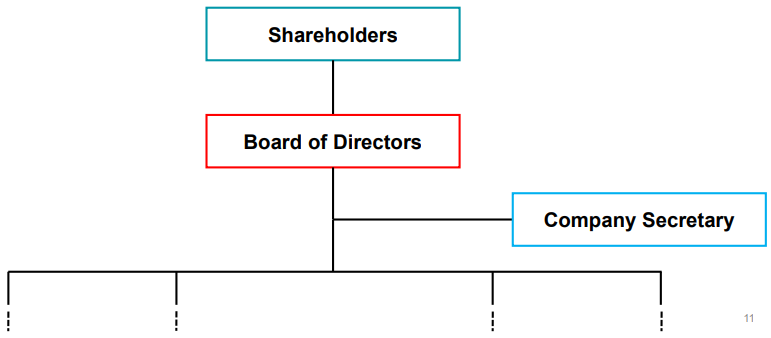
\includegraphics[width = \textwidth]{./img/figure26.png}
    \caption{Structure of a Limited Liability Company limited by shares.}
\end{figure}
\subsection{What is a shareholder?}
\begin{itemize}
    \item Shareholders own a Limited Liability Company limited by shares
    \item They have no day-to-day duties related to the company's operation
    \item Each shareholder owns a fraction of the company (and has corresponding voting power) proportional to their shareholding (investment)
    \item The liability of shareholders is limited to their original investment
    \item The company's profits are paid to shareholders as share dividend
\end{itemize}
\subsection{What is the Board of Directors?}
\begin{itemize}
    \item The Board of Directors is elected by the shareholders at the Annual General Meeting (AGM) to run the company.
          \begin{itemize}
              \item Directors may also be shareholders (but not necessarily)
              \item The shareholders can vote to appoint or sack individual Board of Directors members
          \end{itemize}
    \item The Board of Directors files the company's audited accounts (legal requirement)
    \item The Board of Directors report to the shareholders at the AGM (legal requirement)
    \item The Board of Directors is controller by the Chairman of the Board
    \item The Board of Directors can appoint or sack the Chief Executive Officer (CEO - responsible for day-to-day running)
\end{itemize}
\subsection{What is a company secretary?}
The company secretary ensures the smooth administration of the company. The company secretary is responsible for:
\begin{itemize}
    \item Making sure the company stays within the law
    \item Making sure the company maintains proper record books and accounts
    \item Providing strategic advice to the Board of Directors (sometimes)
\end{itemize}
The company secretary may or may not be a member of the Board of Directors.
\subsection{Limited Liability Company}
A Limited Liability Company that is ``limited by shares'' can be public or private.

Private Limited Company (Ltd.):
\begin{itemize}
    \item Share ownership is controlled
          \begin{itemize}
              \item is owned privately
              \item only one director is required
              \item have nine months to file their annual accounts
              \item a company secretary is not legally required
          \end{itemize}
\end{itemize}

Public Limited Company (PLC):
\begin{itemize}
    \item Share ownership is NOT controlled
          \begin{itemize}
              \item company shares can be bought and sold publically on the open market (a stock exchange)
              \item two directors are required
              \item have six months to file their annual accounts
              \item a company secretary is legally required
          \end{itemize}
\end{itemize}
\section{What is accounting?}
Accounting is the collection, analysis and communication of financial information that is used by:
\begin{itemize}
    \item Those who need to make decisions and plans in an organisation
    \item Those who need to control an organisation
\end{itemize}
Accounting helps companies to plan for the future and evaluate past performance. Accounting os often referred to as the language of business.
\section{The fundamental accounting equation}
\begin{gather}
    \textrm{Assets} = \textrm{Liabilities} + \textrm{Owners' Equity}
\end{gather}
where:
\begin{itemize}
    \item Assets are resources that a company owns. They have the capacity to provide future services or benefits. Companies use their assets in carrying out activities like production and sales
    \item Liabilities are claims against assets - existing debts and obligations. They arise from purchasing items on credit or borrowing money from a bank for purchases
    \item Owners' Equity is what remains of the assets after all liabilities have been paid
\end{itemize}
``Liabilities + Owners' Equity'' are the rights or claims against the resources of the company.
\begin{table}[H]
    \centering
    \begin{tabular}{@{}lll@{}}
        \toprule
        \textbf{Assets} & \textbf{Liabilities} & \textbf{Owners' Equity}\\
        \midrule
        Cash & Wages due & Owners' capital\\
        Equipment & Bank debt &\\
        Buildings & Accounts payable &\\
        Land & & \\
        Inventories & & \\
        \bottomrule
    \end{tabular}  
    \caption{Table to show Assets, Liabilities and Owners' Equity.}  
\end{table}
\subsection{Some important definitions}
\textbf{Assets:}
\begin{quoting}
    Economic resources that a company expects to help generate future cash inflows or help reduce future cash outflow.
\end{quoting}
\textbf{Current assets:}
\begin{quoting}
    A company's cash and other assets that are expected to be converted to cash over the next one year period.
\end{quoting}
\textbf{Non-current assets:}
\begin{quoting}
    A company's assets that are not expected to be converted to cash over the next one year period.
\end{quoting}
\textbf{Inventory:}
\begin{quoting}
    Goods (current assets) available for sale or raw materials and components used to produce goods available for sale.
\end{quoting}
\textbf{Liabilities:}
\begin{quoting}
    Economic obligations of the organisation to outsiders, or claims against its assets by outsiders.
\end{quoting}
\textbf{Current liabilities:}
\begin{quoting}
    A company's short term obligations, due within one year period.
\end{quoting}
\textbf{Non-current liabilities:}
\begin{quoting}
    A company's long-term obligations listed on the balance sheet.
\end{quoting}
\textbf{Dividends:}
\begin{quoting}
    Money paid regularly to shareholders by the company.
\end{quoting}
\section{Balance sheet}
The balance sheet is one of the two most common accounting statements. The fundamental accounting equation defines the format of the balance sheet. The balance sheet shows the financial position of the company at one instant in time (e.g. end of the quarter or end of the year).
\begin{table}[H]
    \centering
    \begin{tabular}{@{}llll@{}}
        \toprule
        Assets              &               & Liabilities / Owners' Equity &               \\
        \midrule
        Cash                & \pounds 2,500 & Accounts payable             & \pounds 1,200 \\
        Land                & \pounds 1,800 & Bank note                    & \pounds 900   \\
        Accounts receivable & \pounds 800   & Owners' Equity               & \pounds 3,000 \\
        \midrule
        Total assets        & \pounds 5,100 & Total liabilities and        & \pounds 5,100 \\
                            &               & Owners' Equity               &               \\
        \bottomrule
    \end{tabular}
    \caption{Balance sheet.}
\end{table}
\begin{gather}
    \textrm{Assets} = \textrm{Liabilities} + \textrm{Owners' Equity} = \pounds 5100
\end{gather}
\section{Income statement}
The income statement is the second of the two most common accounting statements. The income statement summarises the revenue and expense results of operations over a period of time (a moving picture.) It is defined by the following equation:
\begin{gather}
    \textrm{Profit (or Loss)} = \textrm{Revenues} - \textrm{Expenses}
\end{gather}
\begin{table}[H]
    \centering
    \begin{tabular}{@{}llll@{}}
        \toprule
        \textbf{Revenue}    &                &               &               \\
        Sales               &                &               & \pounds 3,000 \\
        \midrule
        \textbf{Expenses}   &                &               &               \\
        Labour              &                & \pounds 1,200 &               \\
        Depreciation        &                & \pounds 400   &               \\
        Material            &                & \pounds 500   &               \\
        \midrule
                            & Total Expenses &               & \pounds 2,100 \\
        \textbf{Net income} &                &               & \pounds 900   \\
        \bottomrule
    \end{tabular}
    \caption{Income statement.}
\end{table}
\subsection{Some important definitions}
\textbf{Turnover:}
\begin{quoting}
    The net sales generated by a business.
\end{quoting}
Turnover and profit are the beginning and end points of the income statement.
\section{Worked example}
John Deere owns and operates a design company called Deere Consulting Ltd. The financial position of his business is:
\begin{table}[H]
    \centering
    \begin{tabular}[]{@{}ll@{}}
        \toprule
        Cash                & \pounds 1,720  \\
        Accounts receivable & \pounds 3,240  \\
        Land                & \pounds 24,100 \\
        Accounts payable    & \pounds 5,400  \\
        John Deere, Capital & \pounds 23,660 \\
        \bottomrule
    \end{tabular}
    \caption{Financial position of John Deere Ltd.}
\end{table}
During May 2021, the following events occurred:
\begin{enumerate}
    \item Deere received \pounds 12,000 as a gift and deposited the cash in the business bank account
    \item Deere paid of the beginning balance of the accounts payable
    \item Deere performed services for a client and received cash of \pounds 1,100
    \item Deere collected \pounds 750 cash from a customer on account
    \item Deere purchased \pounds 720 of supplies on account
    \item Deere billed a client \pounds 5,000 for services rendered
    \item Deere invested personal cash of \pounds 1,700 in the business
    \item Deere recorded \pounds 1,860 of business expenses
    \item Deere sold supplies to another company for \pounds 80 cash (the price of the supplies)
    \item Deere withdrew \pounds 4,000 cash for personal use
\end{enumerate}
For Deere Consulting Ltd., prepare:
\begin{enumerate}
    \item The income statement for the month ended 31 May 2021
    \item The balance sheet as at 31 May 2021
\end{enumerate}
\subsubsection{Income statement, month ended 31 May, 2021}
\begin{table}[H]
    \centering
    \begin{tabular}{@{}llll@{}}
        \toprule
        \textbf{Revenue} & & & \\
        & Services to Client 1 & \pounds 5,000 & \\
        & Services to Client 2 & \pounds 1,100 & \\
        & Total revenue & & \pounds 6,100 \\
        \midrule
        \textbf{Expenses} & & & \\
        & Business expenses & & \pounds 1,860 \\
        \midrule
        \textbf{Net income} & & & \pounds 4,240 \\
        \bottomrule
    \end{tabular}
    \caption{Deere Consulting Ltd. income statement, month ended 31 May, 2021.}
\end{table}
\subsubsection{Balance sheet, 31 May, 2021}
\begin{table}[H]
    \centering
    \begin{tabular}{@{}llll@{}}
        \toprule
        \textbf{Assets} & & \textbf{Liabilities/Owners' Equity}\\
        \midrule
        Cash & \pounds 6,090 & Accounts payable & \pounds 720\\
        Accounts receivable & \pounds 7,490 & & \\
        Supplies & \pounds 640 & & \\
        Land & \pounds 24,100 & J. Deere, Capital & \pounds 37,600 \\
        \midrule
        \textbf{Total assets} & \pounds 38,320 & \textbf{Total liabilities and} & \pounds 38,320\\
        & & \textbf{Owners' Equity} & \\
        \bottomrule
    \end{tabular}
\end{table}
\section{Cash flow statement}
The cash flow statement shows how a ompany generated the cash flows it needed to finance its various opportunities and responsibilities over a period of time (a moving picture). It acts as a bridge between the income statement and the balance sheet by showing how money moved in and out of the business. The cash flow statement has three primary sections:
\begin{enumerate}
    \item Cash flow from operating activities
    \begin{itemize}
        \item Cash inflows: generation of funds in normal operations
        \item Cash outflows: expenduture of funds in normal operations
    \end{itemize}
    \item Cash flow from investing activities
    \begin{itemize}
        \item Cash inflows: sale of plant and equipment. Liquidation of long-term investment
        \item Cash outflows: purchase of plant and equipment. Long-term investments
    \end{itemize}
    \item Cash flow from financing activities
    \begin{itemize}
        \item Cash inflows: sale of bonds, common stock and other securities
        \item Csh outflows: repurchase of bonds, common stock and other securities. Payment of cash dividend
    \end{itemize}
\end{enumerate}
The sum of these sections = net cash flow.
\subsection{Cash flow statement}
\begin{table}[H]
    \centering
    \begin{tabular}{@{}ll@{}}
        \toprule
        \textbf{Cash flows from operating activities} & \\
        Cash generated from operations & \pounds 5,460\\
        Income tax paid & -\pounds 1,351\\
        Interest paid & -\pounds 40\\
        \midrule
        Net cash flow from operating activities & \pounds 4,069\\
        \midrule
        \textbf{Cash flows from investing activities} & \\
        Interest received & \pounds 100\\
        Purchases of property, plant and equipment & \pounds 5,894\\
        Proceeds on disposal of property & \pounds 41\\
        Capital grants received & \pounds 1,979\\
        \midrule
        Net cash flow from investing activities & -\pounds 3,774\\
        \midrule
        \textbf{Cash flows from financing activities} & \\
        Repayments of borrowings & -\pounds 10,991\\
        New loans raised & \pounds 10,841\\
        Repayment of liase liabilities & -\pounds 107\\
        \midrule
        Net cash flow from financing activities & -\pounds 257\\
        \midrule
        Net increase/(decrease) in cash and cash equivalents & \pounds 38\\
        Cash and cash equivalents at beginning of the period & \pounds 430\\
        \midrule
        \textbf{Cash and cash equivalents at end of year} & \pounds 522\\
        \bottomrule
    \end{tabular}
    \caption{Cash flow statement.}
\end{table}
\subsection{Financial ratios}
Financial ratios are mathematical calculations that a company can use to evaluate its performance. They are relative magnitudes of selected numerical values taken from a company's financial statements. Financial ratios may be used by managers, stakeholders or creditors to:
\begin{itemize}
    \item Determine whether key performance trends are improving or not
    \item Compare ratios (and therefore company performances) between years
    \item Define goals for future companies
\end{itemize}
Financial analysts use financial ratios to compare strengths and weaknesses across various companies. There are five different types of financial ratios:
\begin{enumerate}
    \item Liquidity ratios - help evaluate a company's ability to pay its bills on a regular week-to-week or month-to-month basis
    \item Financial leverage ratios - measure how much of a company's assets belong to the shareholders rather than creditors (lenders)
    \item Asset utility ratios - measure how efficient a company is with using its assets to generate revenue
    \item Profitability ratios - help evaluate how well the firm generates a profit through its operations
    \item Market value ratios - help evaluate the economic status of publicly traded companies and can play a role in identifying stocks that may be overvalued, undervalued or priced fairly
\end{enumerate}
\subsubsection{Liquidity ratios}
\textbf{Current ratio} - measure the ability to pay short-term debt. If Current ratio $<$ 1, the company has liquidity problems to cover its short-term liabilities. If Current ratio = 1, the company is able to cover its short-term liabilities. The ideal Current ratio is between 1.2 and 2.
\begin{gather}
    \textrm{Current ratio} = \frac{\textrm{Current assets}}{\textrm{Current liabilities}}
\end{gather}

\textbf{Quick ratio} - measure the ability to pay short-term debt. If Quick ratio $<$ 1, the company finds it hard to fully pay its debt in the short term. If Quick ratio $>$ 1, the company is able to cover its debt.
\begin{gather}
    \textrm{Quick ratio} = \frac{\textrm{Current assets}-\textrm{Inventory}}{\textrm{Current liabilities}}
\end{gather}

\textbf{Cash ratio} - measure the ability of cash to pay debt. If Cash ratio $<$ 1, there is insufficient cash to pay off short-term debt. If Cash ratio = 1, there is sufficient cash to pay off short-term debt. If Cash ratio $>$ 1, there is more than sufficient cash to pay off short-term debt.
\begin{gather}
    \textrm{Cash ratio} = \frac{\textrm{Cash}}{\textrm{Current liabilities}}
\end{gather}
\subsubsection{Financial leverage ratios}
\textbf{Total debt ratio} - measure the degree to which a company has used debt to finance its assets. Total Debt ratio quantifies the proportion of company financing that comes from creditors.
\begin{gather}
    \textrm{Total Debt ratio} = \frac{\textrm{Total assets} - \textrm{Total equity}}{\textrm{Current Assets}}
\end{gather}

\textbf{Debt-Equity ratio} - measure the degree to which shareholder equity covers all outstanding debts. Debt-Equity ratio quantifies the proportion of company financing that comes from investors.
\begin{gather}
    \textrm{Debt=Equity ratio} = \frac{\textrm{Total liabilities}}{\textrm{Total equity}}
\end{gather}

\textbf{Equity Multiplier ratio} - measure the degree to which stakeholder equity covers the company's assets. Equity Multiplier ratio quantifies the proportion of a company's assets that is financed by stakeholder equity.
\begin{gather}
    \textrm{Equity Multiplier ratio} = \frac{\textrm{Total assets}}{\textrm{Total equity}}
\end{gather}

\textbf{Times Interest Earned ratio} - measure the creditworthiness of a company (the ability of the company to meet its debts). Earning before interest and taxes can be abbreviated as EBIT. Times Interest Earned ratio quantifies the number of times a company could pay the interest on its annual debt.
\begin{gather}
    \textrm{Times Interest Earned ratio} = \frac{\textrm{Earning before interest and taxes}}{\textrm{Interest}}
\end{gather}

\textbf{Cash Coverage ratio} - measure the ability of a company to service its debt and meet financial obligations (e.g. interest payments and dividend). Cash Coverage ratio quantifies the cash available to a company as a proportion of the interest on its annual debt.
\begin{gather}
    \textrm{Cash Coverage ratio} = \frac{\textrm{EBIT} + \textrm{Non}-\textrm{Cash Expenses}}{\textrm{Interest}}
\end{gather}
\subsubsection{Asset utility ratios}
\textbf{Inventory turnover} - measure how efficiently a company manages its inventory. Inventory is defined here as average inventory over the course of the period. Inventory turnover quantifies the number of times an inventory is created and sold during the period.
\begin{gather}
    \textrm{Inventory turnover} = \frac{\textrm{Cost of goods sold}}{\textrm{Inventory}}
\end{gather}

\textbf{Day sales in inventory} - measure how long a company's stock of inventory will last. Day sales in inventory quantifies the average time in days that a company takes to turn its inventory into sales.
\begin{gather}
    \textrm{Day sales in inventory} = \frac{365}{\textrm{Inventory turnover}}
\end{gather}

\textbf{Receivables turnover} - measure how quickly a company is collecting its sales that were made on credit. Receivables turnover quantifies the number of times ``accounts receivable'' have been created through the sale of goods on credit.
\begin{gather}
    \textrm{Receivables turnover} = \frac{\textrm{Net annual credit sales}}{\textrm{Accounts receivable}}
\end{gather}

\textbf{Day sales in accounts receivable} - measure how quickly a company is collecting cash from its credit sales. Day sales in accounts receivable quantifies the average time in days that a company takes to collect cash from its credit sales.
\begin{gather}
    \textrm{Day sales in accounts receivable} = \frac{365}{\textrm{Receivable turnover}}
\end{gather}

\textbf{Total asset turnover ratio} - measures the value of a company's sales or revenues relative to its assets. Total asset turnover ratio quantifies the size of total sales as a proportion asset investment.
\begin{gather}
    \textrm{Total asset turnover ratio} = \frac{\textrm{Total annual sales}}{\textrm{Total assets}}
\end{gather}

\textbf{Capital intensity ratio} - measures the amount of assets requires to generate \pounds 1 in sales. Capital intensity ratio quantifies the size of asset investment as a proportion of total sales.
\begin{gather}
    \textrm{Capital intensity ratio} = \frac{\textrm{Total assets}}{\textrm{Total annual sales}}
\end{gather}
\subsubsection{Profitability ratios}
\textbf{Profit margin} - measures the degree to which a company makes money. Profit margin quantifies the proportion sales that has turned into profit.
\begin{gather}
    \textrm{Profit margin} = \frac{\textrm{Net income}}{\textrm{Net sales}}
\end{gather}

\textbf{Return on assets ratio} - measures a company's net income produced from its total assets. Return on assets ratio quantifies company income as a proportion of its total assets.
\begin{gather}
    \textrm{Return on assets ratio} = \frac{\textrm{Net income}}{\textrm{Total assets}}
\end{gather}

\textbf{Return on equity ratio} - measures the return a company makes on its equity. Return on assets ratio quantifies net income as a proportion of shareholder equity.
\begin{gather}
    \textrm{Return on equity ratio} = \frac{\textrm{Net income}}{\textrm{Total equity}}
\end{gather}
\subsubsection{Market value ratios}
Note: 
\begin{itemize}
    \item Shares are units of equity ownership in a company
    \item Stocks are the same as shares
    \item A stock exhange is a market that matches buyers of company shares with sellers of company shares
    \item A financial market is a place where financial assets are issues and traded
\end{itemize}
\textbf{Price-earnings ratio} - measures whether a company's stock price is overvalued or undervalued. Price-earnings ratio quantifies current share price as a proportion of profit per share.
\begin{gather}
    \textrm{Price-earnings ratio} = \frac{\textrm{Price per share}}{\textrm{Earnings per share}}
\end{gather}

\textbf{Market-to-book ratio} - measures whether a company is overvalued or undervalued. Here, Market value per share is the stock price (worth on the market) and Book value per share is the amount of money left if all assets are sold and all liabilities are paid. Market-to-book ratio quantifies a company's current market value relative to its book value.
\begin{gather}
    \textrm{Market-to-book ratio} = \frac{\textrm{Market value per share}}{\textrm{Book value per share}}
\end{gather}
\chapter{Critical Path and Delay Analysis in Construction Projects}
\section{Kroll Expert Services}
With experience spanning global industries across the world's continents, we are a market leader for expert witnesses, dispute resolution, advisory and investigative services. Our clients include international contractor, government agencies, blue chip multinationals, investors, developers, banks and insurers.
\begin{itemize}
    \item Delay analysis
          \begin{itemize}
              \item The assessment of the incidence, extent and causes of delay to the progress and completion of capital investment projects
          \end{itemize}
    \item Quantum analysis
          \begin{itemize}
              \item Construction quantum is the assessment of financial entitlement of the parties arising from claims under or out of a construction contract
          \end{itemize}
    \item Project advisory
          \begin{itemize}
              \item Our advisory practice draws on our in-depth project delivery, management and industry expert insight to provide pre-dispute advisory services to capital projects, infrastructure programmes and real assets organisations across their delivery lifecycle
          \end{itemize}
\end{itemize}
\section{Dispute in construction and the role of experts}
\subsection{What is a dispute?}
\begin{figure}[H]
    \centering
    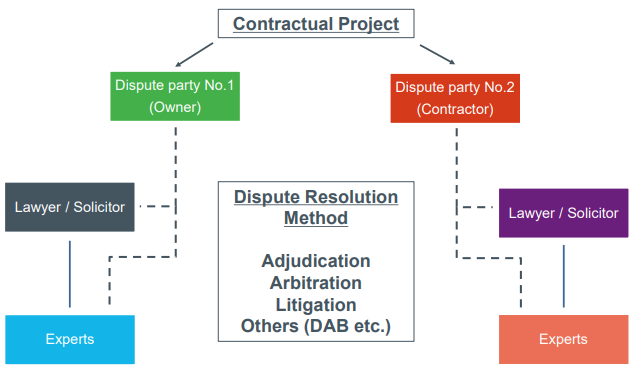
\includegraphics[width = 0.8\textwidth]{img/figure27.png}
    \caption{Dispute pathway.}
\end{figure}
\subsection{Typical sequence to a trial}
\begin{enumerate}
    \item Dispute arises between two parties
    \item Dispute party hires a lawyer
    \item Lawyer engages with an independent expert
    \item Dispute party provides the expert with evidence
          \begin{itemize}
              \item Identify issues
              \item Analyse data
              \item Prioritise key areas
          \end{itemize}
    \item The expert provides independent expert report
          \begin{itemize}
              \item Report could be used:
              \item in dispute resolution
              \item for consulting purposes
              \item for negotiation purposes
          \end{itemize}
    \item Engage with opposing expert
    \item Go to trial
          \begin{itemize}
              \item Oral evidence / cross examination
          \end{itemize}
\end{enumerate}
\subsection{Independent expert}
\begin{itemize}
    \item Independent
          \begin{itemize}
              \item An expert witness is to provide \textbf{independent}, impartial and unbiased evidence to the court or tribunal
          \end{itemize}
    \item Expert
          \begin{itemize}
              \item An \textbf{expert} is a person engages to give an opinion based on experience, knowledge and expertise
          \end{itemize}
    \item Assist
          \begin{itemize}
              \item The primary duty of an expert witness is to \textbf{assist} the court
          \end{itemize}
\end{itemize}
\section{Critical path and delay analysis}
\subsection{What is delay analysis?}
Definition:
\begin{quoting}
    Delay analysis is the assessment of impact, \textbf{causes} and \textbf{effects} of a construction or engineering project not meeting its original forecast completion date.
\end{quoting}
Delay analysis includes:
\begin{itemize}
    \item Determination of critical path of the project (EFFECT)
    \item Assessment of extent of delays (quantification of EFFECT)
    \item Assessment of causes of delays (CAUSE)
\end{itemize}
\subsection{What is the critical path?}
\begin{quoting}
    The longest sequence of activities through a project network from start to finish, the sum of whose durations determines the overall project duration.
\end{quoting}
\subsection{Basics of delay}
\begin{figure}[H]
    \centering
    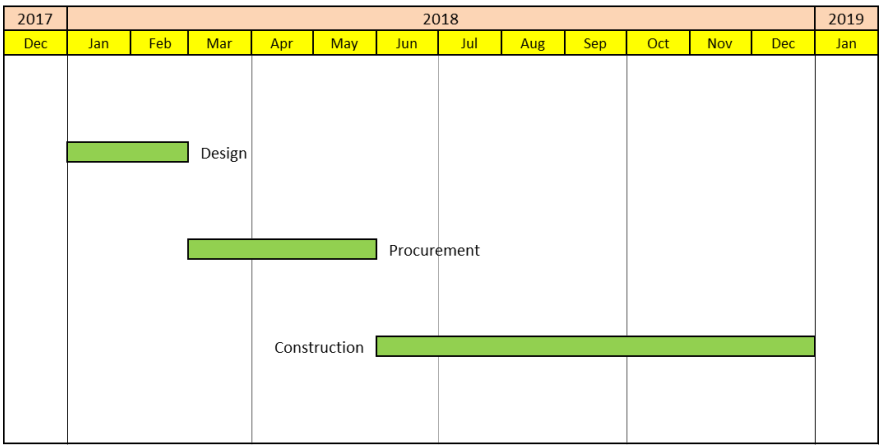
\includegraphics[width = 0.8\textwidth]{img/figure28.png}
    \caption{Work programmes can be as simple as a few bar charts.}
\end{figure}
\begin{figure}[H]
    \centering
    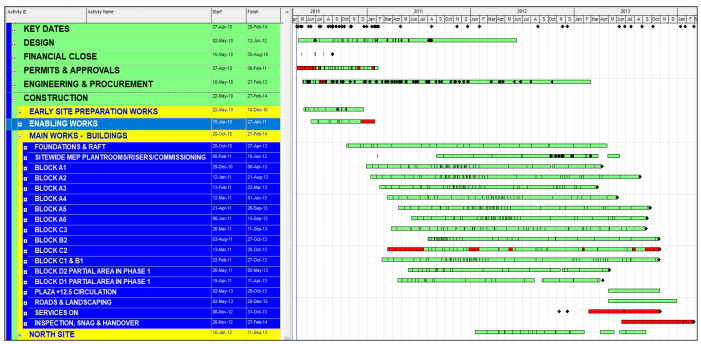
\includegraphics[width = 0.8\textwidth]{img/figure29.png}
    \caption{Or a complex schedule prepared in a specialist software.}
\end{figure}
\subsection{Information sources}
Experts do not just rely on the programme. The best intelligently utilise other as-built evidence. A key rule:
\begin{quoting}
    Never rely on assumptions when you know the facts.
\end{quoting}
\begin{itemize}
    \item Primary
          \begin{itemize}
              \item Photographs
              \item Videos
              \item Site diaries / daily reports
              \item Pour / installation records
              \item Inspection sheets
              \item Daily allocation sheets L/P/M
              \item Detailed timesheets / labour resources timesheets
              \item Detailed sign-off sheets
              \item Detailed quality records
              \item Contemporaneously marked-up progress drawings
              \item Quality Assurance documentation
          \end{itemize}
    \item Secondary
          \begin{itemize}
              \item Updated programmes
              \item Look-ahead programmes
              \item Progress reports
              \item Progress meetings' minutes
              \item Data spreadsheets
              \item Valuations / earned value analysis
              \item As-built drawings / records
              \item Claims
          \end{itemize}
    \item Tertiary
          \begin{itemize}
              \item Correspondence
              \item General meeting minutes
              \item RFIs (Request for Inspections)
              \item TQs (Technical Queries)
              \item Variations / Changes of Orders
              \item Instructions
              \item Etcetera
          \end{itemize}
\end{itemize}
\subsection{Methods of delay analysis}
\begin{table}[H]
    \centering
    \begin{tabular}{@{}llll@{}}
        \toprule
        \textbf{Method of analysis}             & \textbf{Analysis type} & \textbf{Critical path determined} & \textbf{Delay impact determined} \\
        \midrule
        Impacted as-planned analysis            & Cause \& Effect        & Prospectively                     & Prospectively                    \\
        Time impact analysis                    & Cause \& Effect        & Contemporaneously                 & Prospectively                    \\
        Time slice windows analysis             & Effect \& Cause        & Contemporaneously                 & Retrospectively                  \\
        As-planned vs as-built windows analysis & Effect \& Cause        & Contemporaneously                 & Retrospectively                  \\
        Longest path analysis                   & Effect \& Cause        & Retrospectively                   & Retrospectively                  \\
        Collapsed as-built analysis             & Cause \& Effect        & Retrospectively                   & Retrospectively                  \\
        \bottomrule
    \end{tabular}
    \caption{Methods of delay analysis.}
\end{table}
\subsection{Example 1}
Consider two buildings:
\begin{figure}[H]
    \centering
    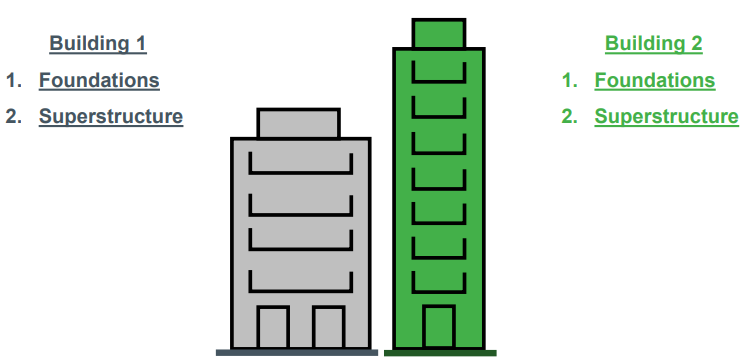
\includegraphics[width = 0.8\textwidth]{img/figure30.png}
    \caption{Example project with two buildings.}
\end{figure}
\subsubsection{Impact as-planned analysis}
Potential issue with the result we get as it is all perspective. None of the sequence happened as it should have. Everything in green is a projection i.e. what should have happened. Impacting what should happen is not consistent with the real world events. For example, in this example, we could add mitigation to the superstructure of B2, moving the project completion to the left (shortening it).

Another issue is that results are quite biased. Using this method, we tend to maximise the impact of delay, so any introduction of a delay event is likely to cause a delay in the completion date, regardless of whether it is critical or not. We have not found a true critical path to impact the delay onto it.

Another issue is that we are only picking certain delay events and not necessarily taking into account other delay events. In this example, we have only taken a delay event for B2. There could be other things happening in B1 that we are not taking into account. This analysis tends to favour the party selecting the events to be modelled; it could be ignoring delay events that are not favourable to the client or the contractor.
\begin{figure}[H]
    \centering
    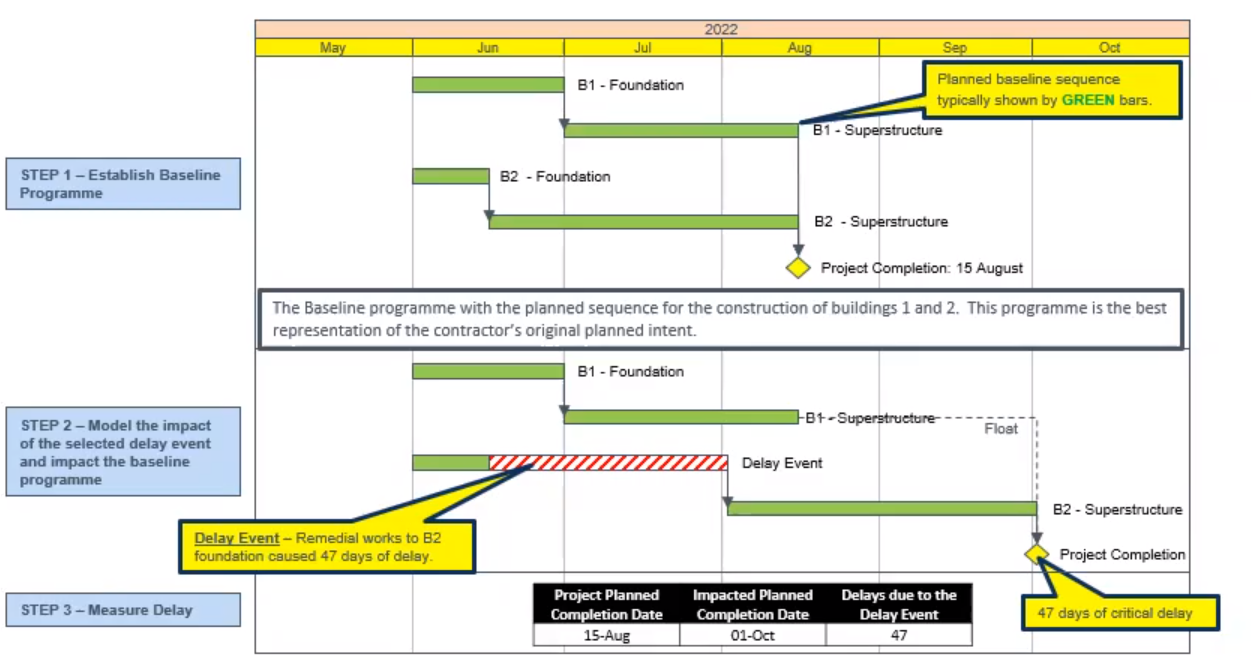
\includegraphics[width = \textwidth]{img/figure31.png}
    \caption{Impact as-planned analysis for example project.}
\end{figure}
\subsubsection{Time impact analysis}
This differs from Impact as-planned analysis, as we take into consideration actual progress on the project, represented by the blue bars. Similarly to the previous analysis method, it is still a matter of perspective. We are still projecting the completion date. Again, we can pick certain delay events that are not necessarily taking into account the full impact of other delay events on the other buildings. However, this analysis method is reliable in anticipating the potential delay of an event. This is a method used on live projects that have not been finished yet to predict delay impact.
\begin{figure}[H]
    \centering
    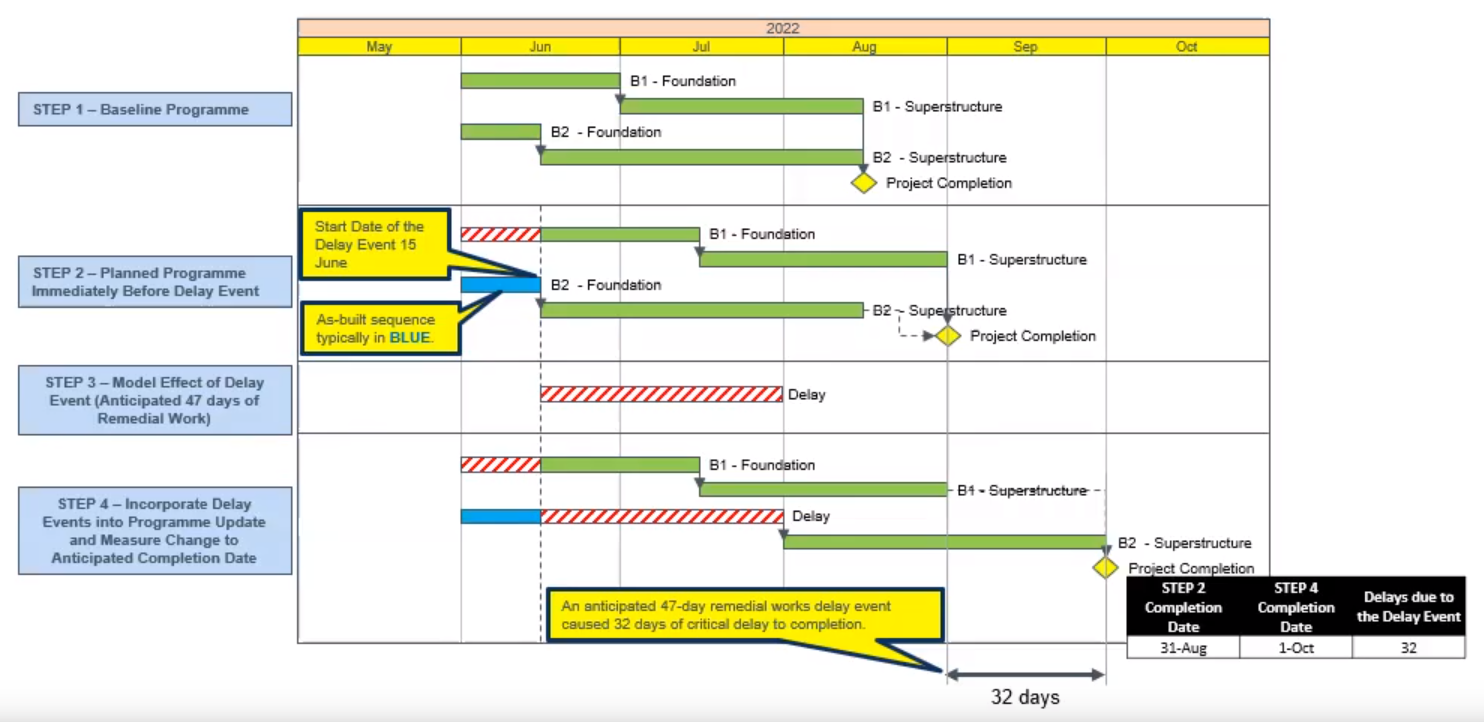
\includegraphics[width = \textwidth]{img/figure32.png}
    \caption{Time impact analysis for example project.}
\end{figure}
\subsubsection{Time slice windows analysis}
This method takes into account all that happened during the project. It takes into account all the ongoing parallel issues and makes an assessment of whether it is critical or not. It is quite an accurate method of delay and is used on projects. An issue is that it relies very heavily on programme updates. This could mean it is heavily biased; in the construction programme the contractor may use it to artificially establish an entitlement for an extension of time. This means that the information provided could be skewed to favour the contractor. In ideal circumstances, when we have an ideal programme and we find it is not biased or it has not been used at all by the contractor, we can use this form of analysis, to analyse delay. However, the case is usually that they are not reliable.
\begin{figure}[H]
    \centering
    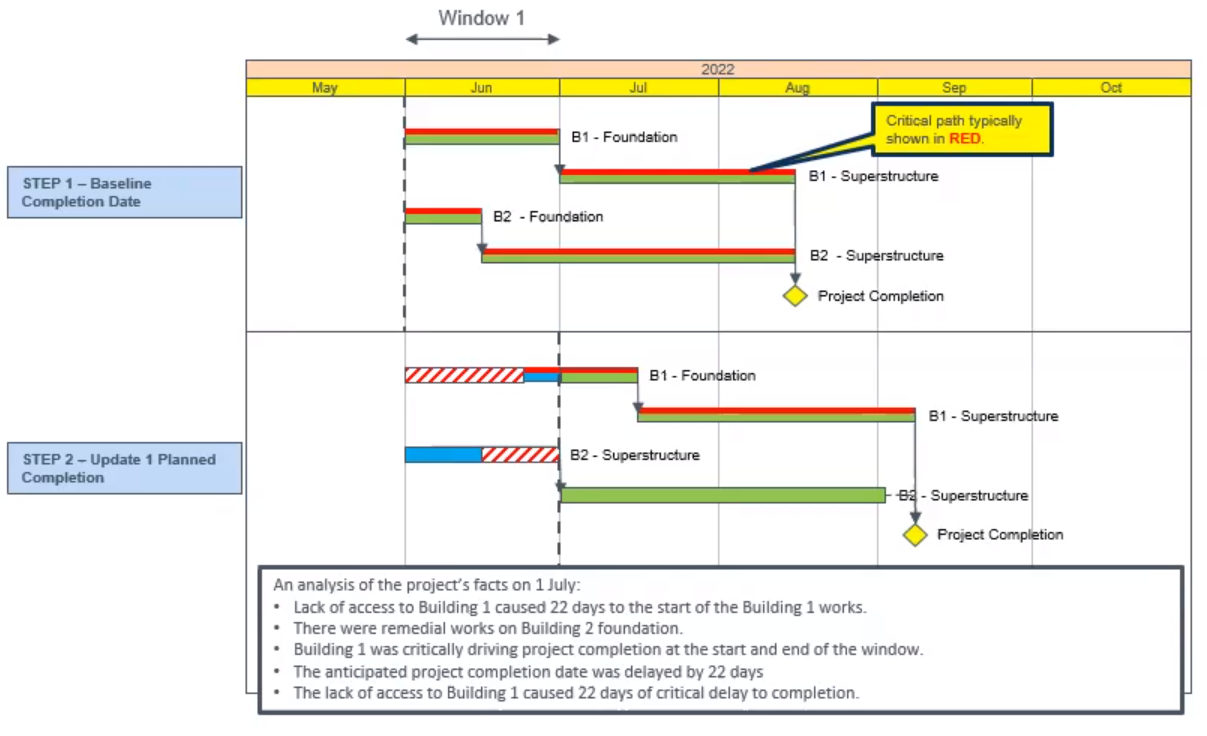
\includegraphics[width = \textwidth]{img/figure33.png}
    \caption{Time slice windows analysis for example project. Window 1}
\end{figure}
\begin{figure}[H]
    \centering
    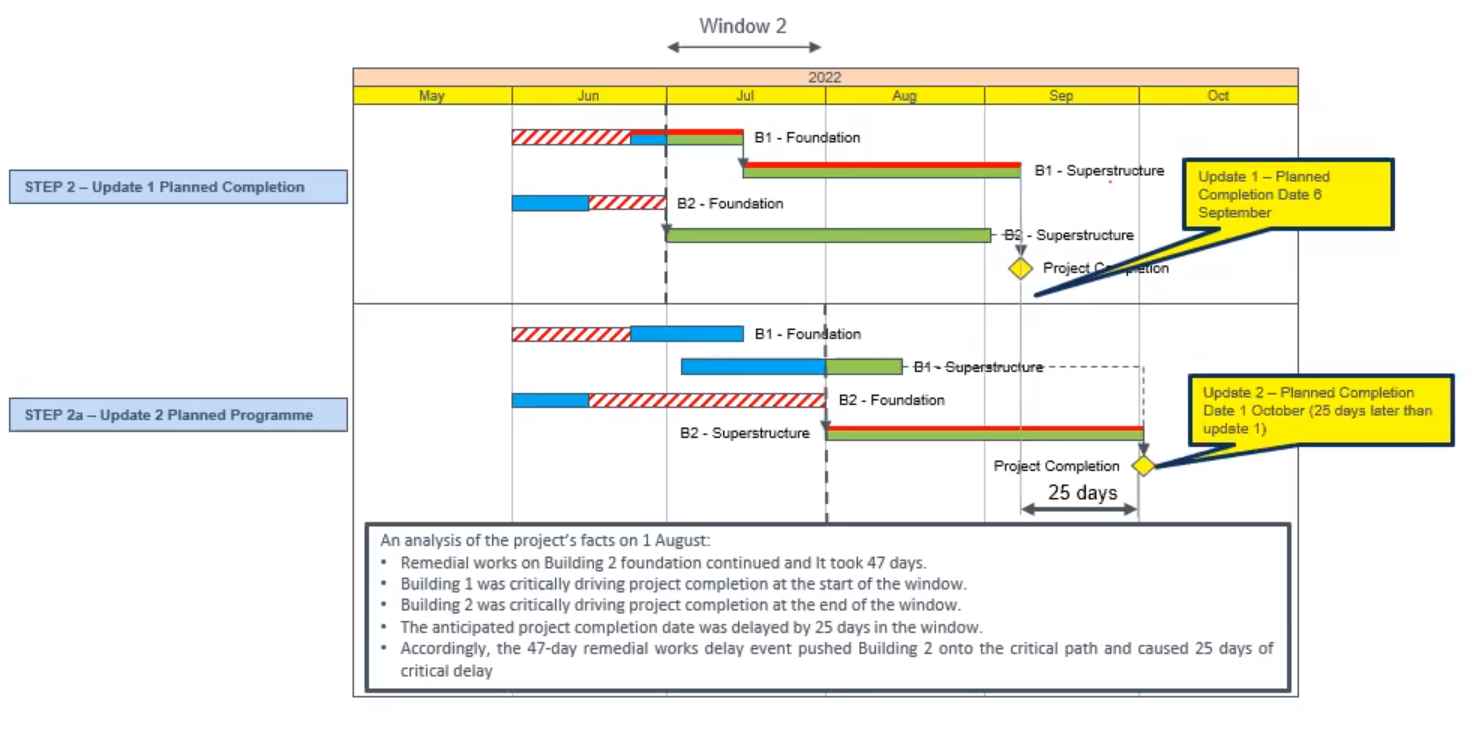
\includegraphics[width = \textwidth]{img/figure34.png}
    \caption{Time slice windows analysis for example project. Window 2.}
\end{figure}
\begin{figure}[H]
    \centering
    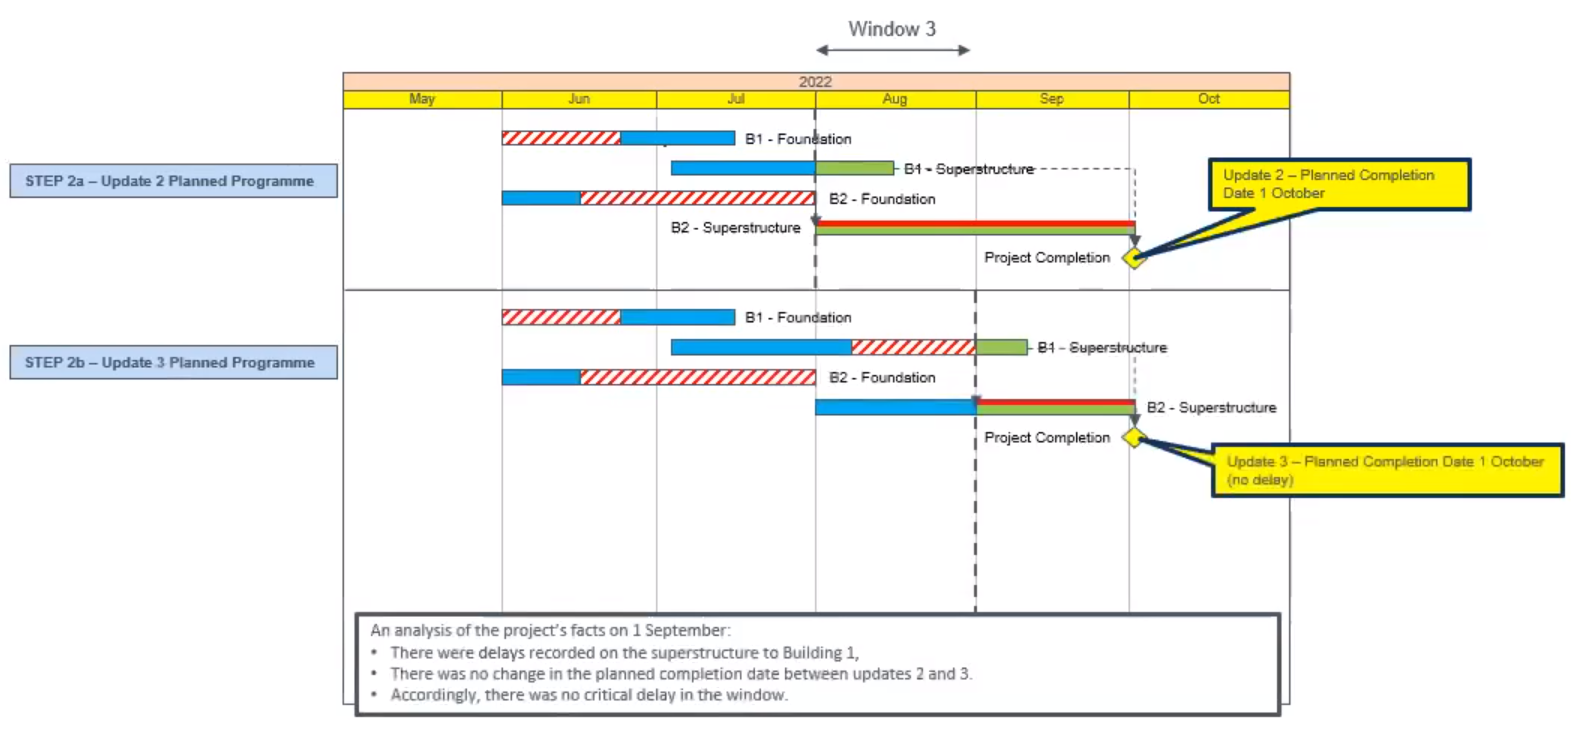
\includegraphics[width = \textwidth]{img/figure35.png}
    \caption{Time slice windows analysis for example project. Window 3.}
\end{figure}
\begin{figure}[H]
    \centering
    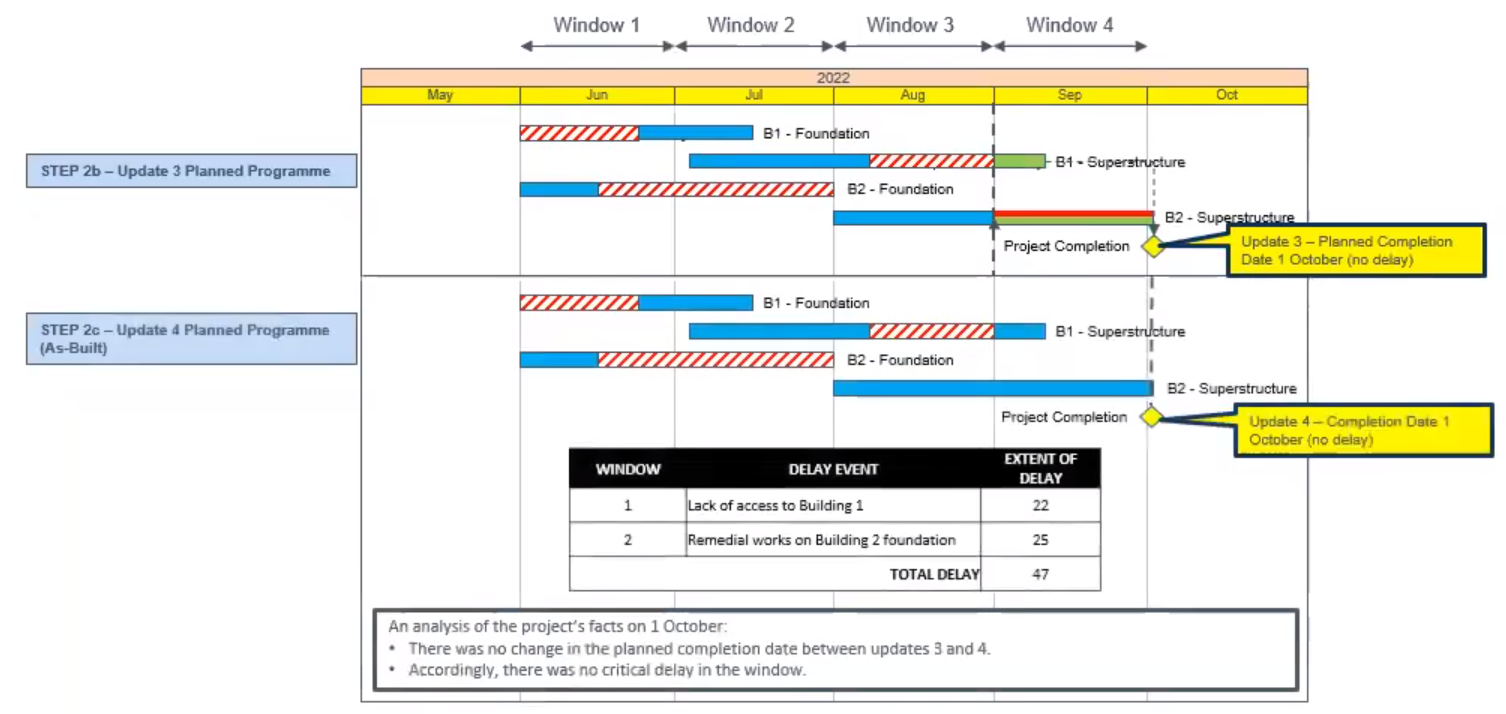
\includegraphics[width = \textwidth]{img/figure36.png}
    \caption{Time slice windows analysis for example project. Window 4.}
\end{figure}
\subsubsection{As-planned vs as-built windows analysis}
More effort is required for this analysis. This is usually the best method to use, however a key issue with this method is that all delays are measured against the baseline programme. This can lead to dispute if the baseline programme is quite wrong and unfeasible. A skewed baseline programme would lead to skewed delay results.

This method of analysis defines the critical path through experience and looking through the data, which is something more difficult to defend, because as an expert, you are relying your own subjective opinion to determine the critical path. Lawyers or disputing parties may argue against this. It also requires the project data to be reliable.
\begin{figure}[H]
    \centering
    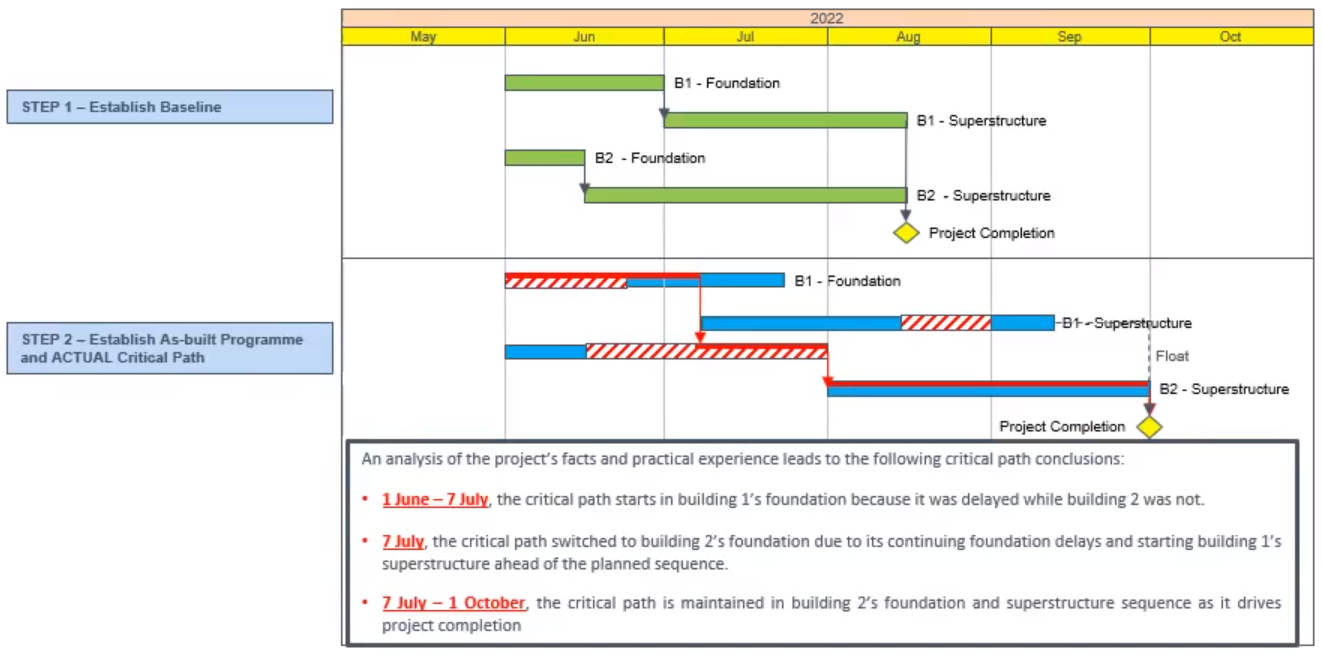
\includegraphics[width = \textwidth]{img/figure37.png}
    \caption{As-planned vs as-built windows analysis for example project. Step 1 \& 2.}
\end{figure}
\begin{figure}[H]
    \centering
    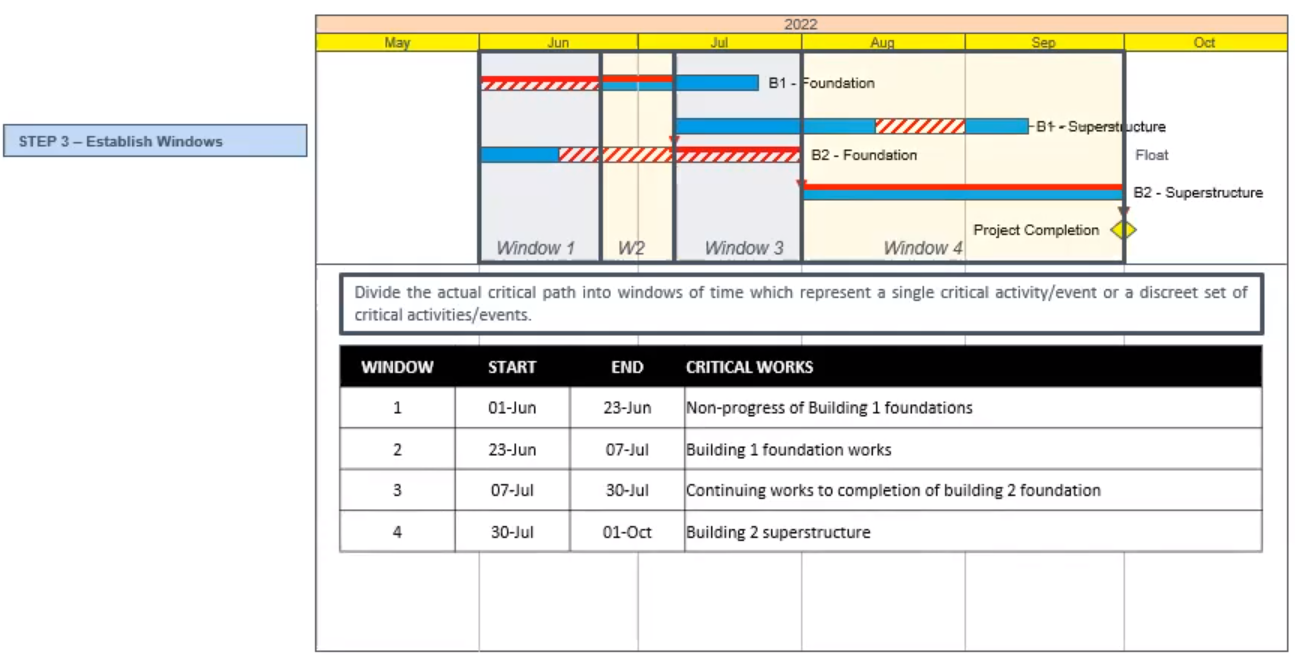
\includegraphics[width = \textwidth]{img/figure38.png}
    \caption{As-planned vs as-built windows analysis for example project. Step 3.}
\end{figure}
\begin{figure}[H]
    \centering
    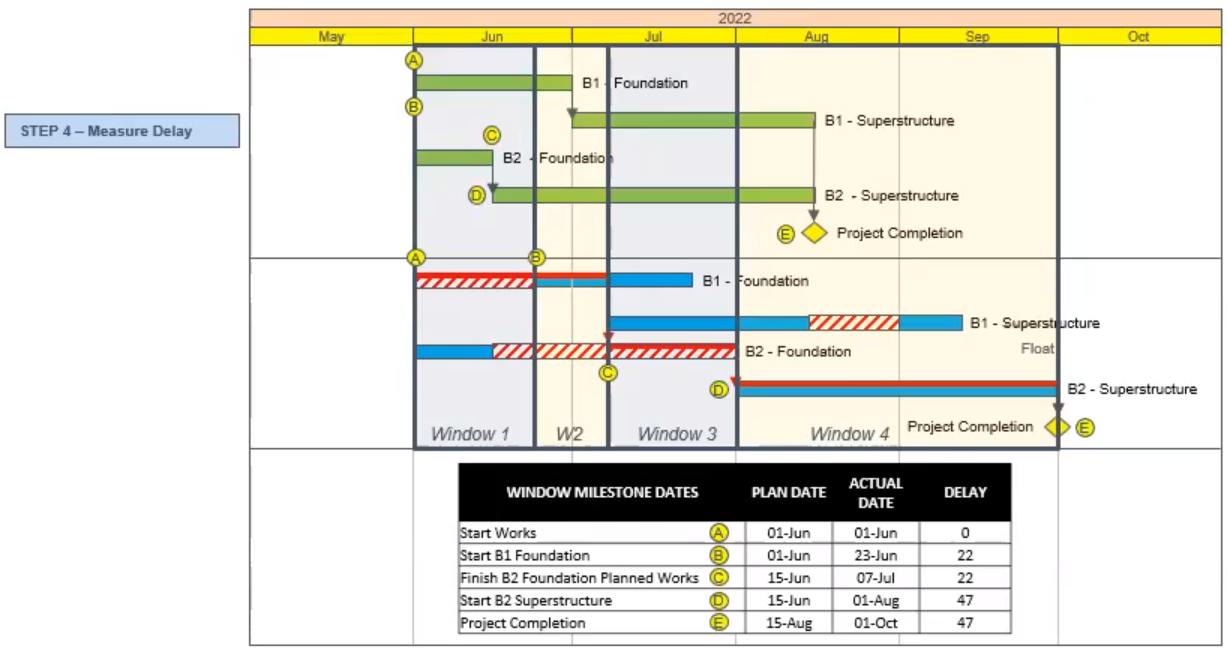
\includegraphics[width = \textwidth]{img/figure39.png}
    \caption{As-planned vs as-built windows analysis for example project. Step 4.}
\end{figure}
\begin{figure}[H]
    \centering
    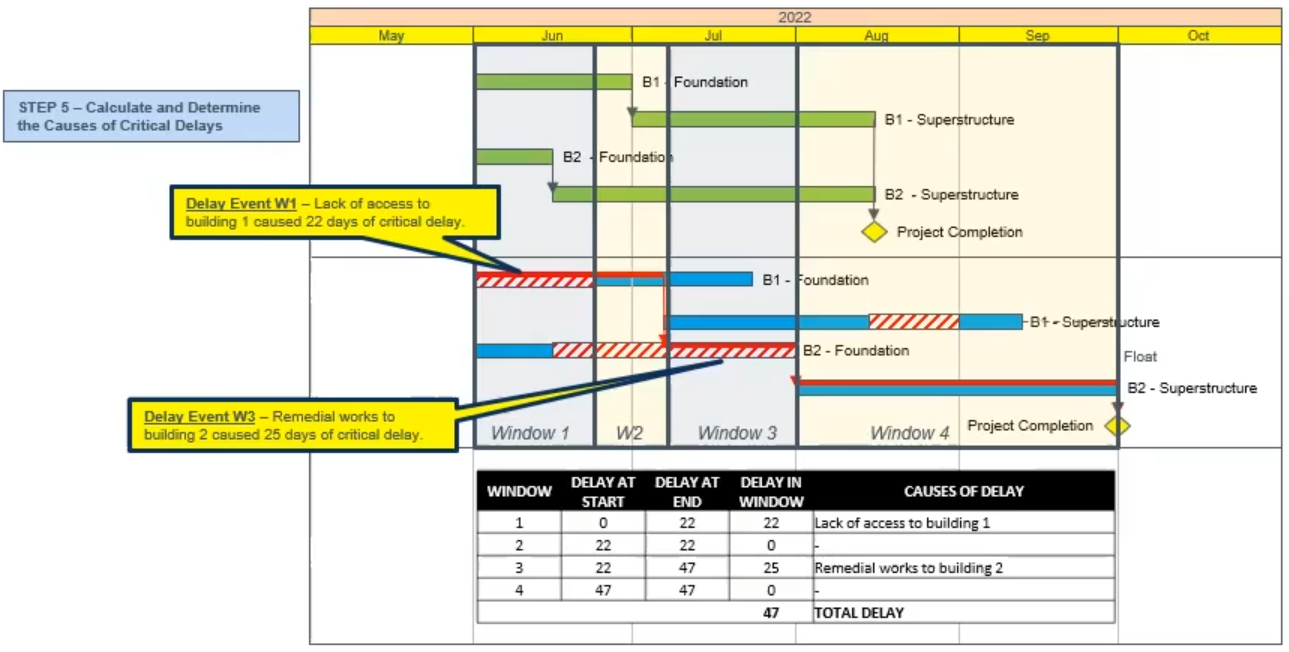
\includegraphics[width = \textwidth]{img/figure40.png}
    \caption{As-planned vs as-built windows analysis for example project. Step 5.}
\end{figure}
\subsubsection{Longest path analysis}
Here, the critical path is found retrospectively, which does not really allow for the switching of the critical path between the two buildings. Usually, in large projects, the critical path switches between many different aspects of the project. In a simple project, this type of analysis might work. For larger projects, we do need to analyse the critical path more contemporaneously. This method of analysis is sometimes used when programme updates are too few or unreasonable, which prevents the use of time slice windows.
\begin{figure}[H]
    \centering
    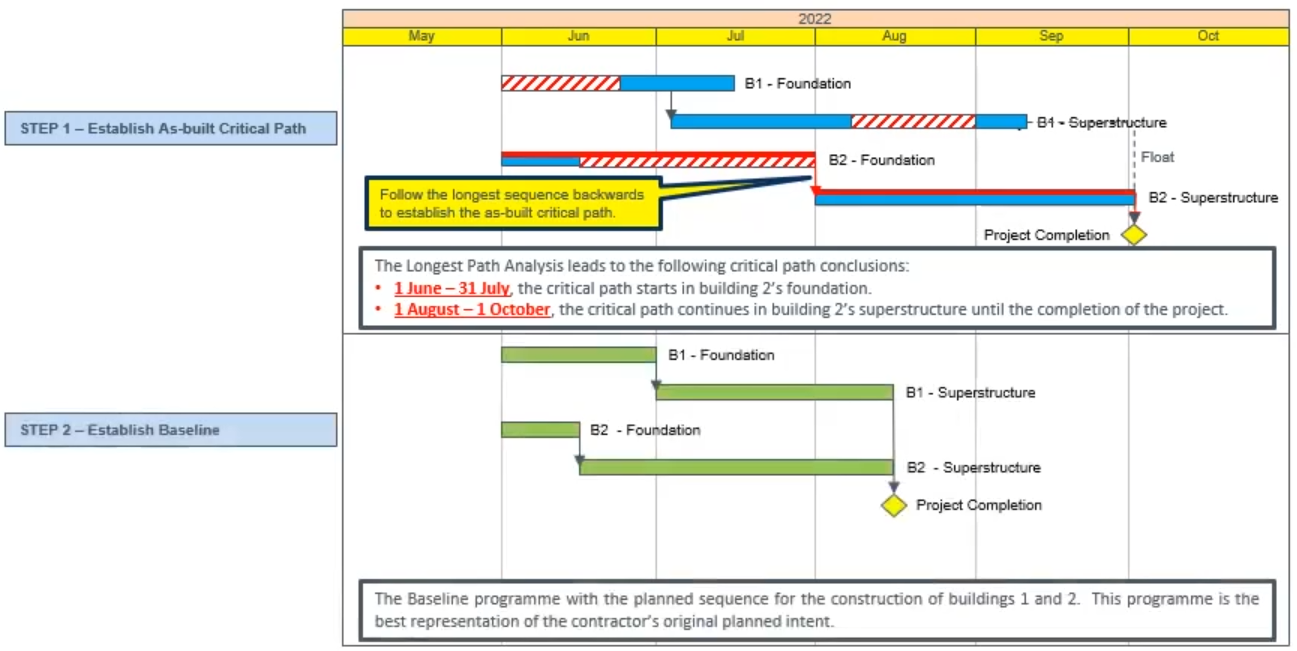
\includegraphics[width = \textwidth]{img/figure41.png}
    \caption{Longest path analysis for example project. Step 1 \& 2.}
\end{figure}
\begin{figure}[H]
    \centering
    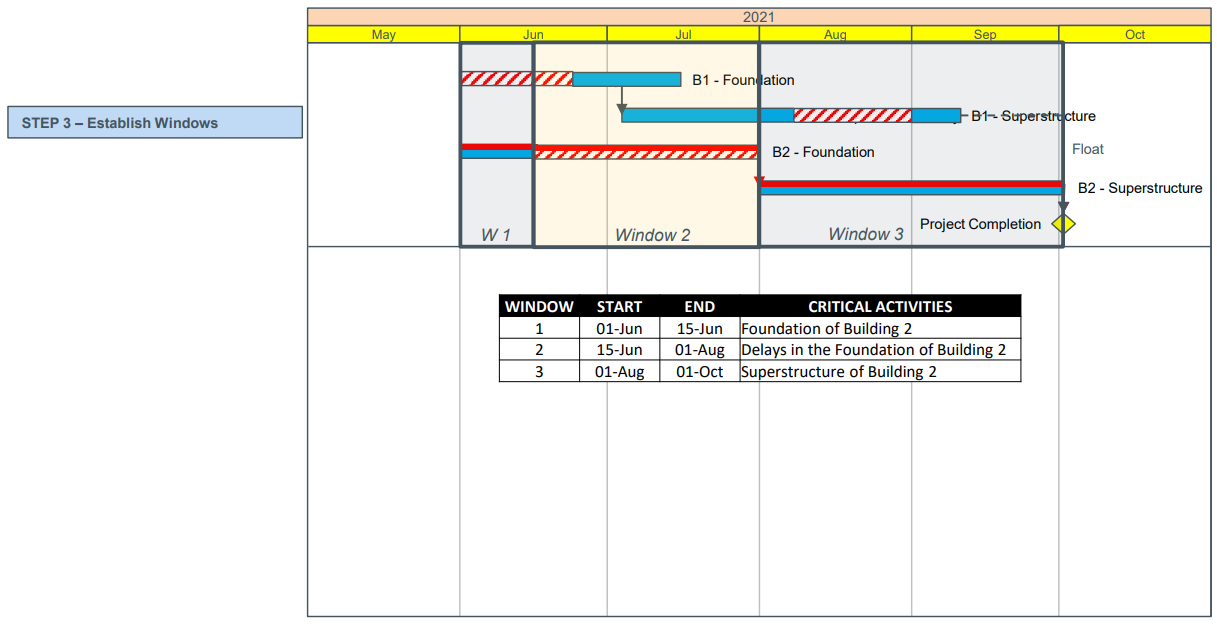
\includegraphics[width = \textwidth]{img/figure42.png}
    \caption{Longest path analysis for example project. Step 3.}
\end{figure}
\begin{figure}[H]
    \centering
    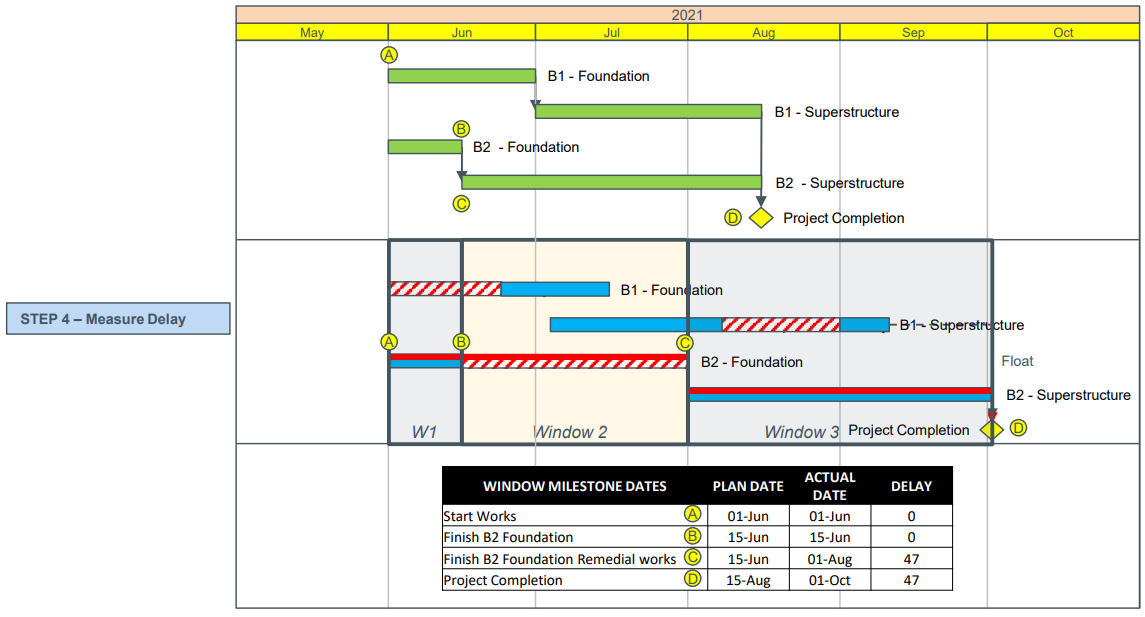
\includegraphics[width = \textwidth]{img/figure43.png}
    \caption{Longest path analysis for example project. Step 4.}
\end{figure}
\begin{figure}[H]
    \centering
    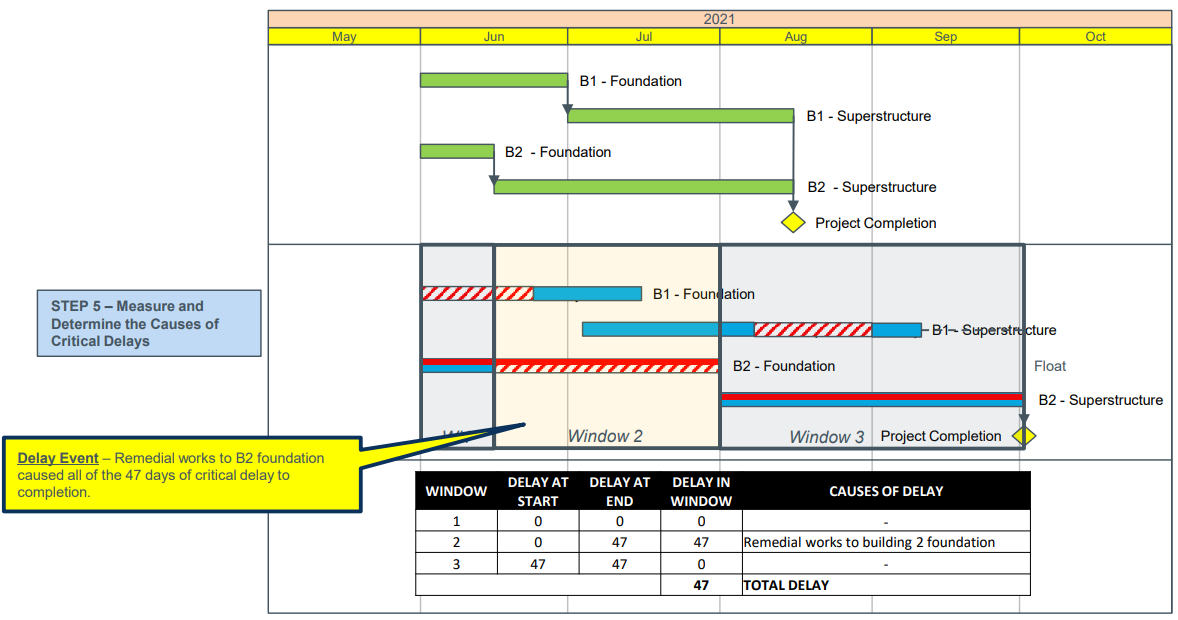
\includegraphics[width = \textwidth]{img/figure44.png}
    \caption{Longest path analysis for example project. Step 5.}
\end{figure}
\subsubsection{Collapsed as-built analysis}
This involves building a programme from scratch using the project records (as-built data) and track what happened in the project. Then we can add in our delay events, and calculate the projected completion date if there was no delay.
\begin{figure}[H]
    \centering
    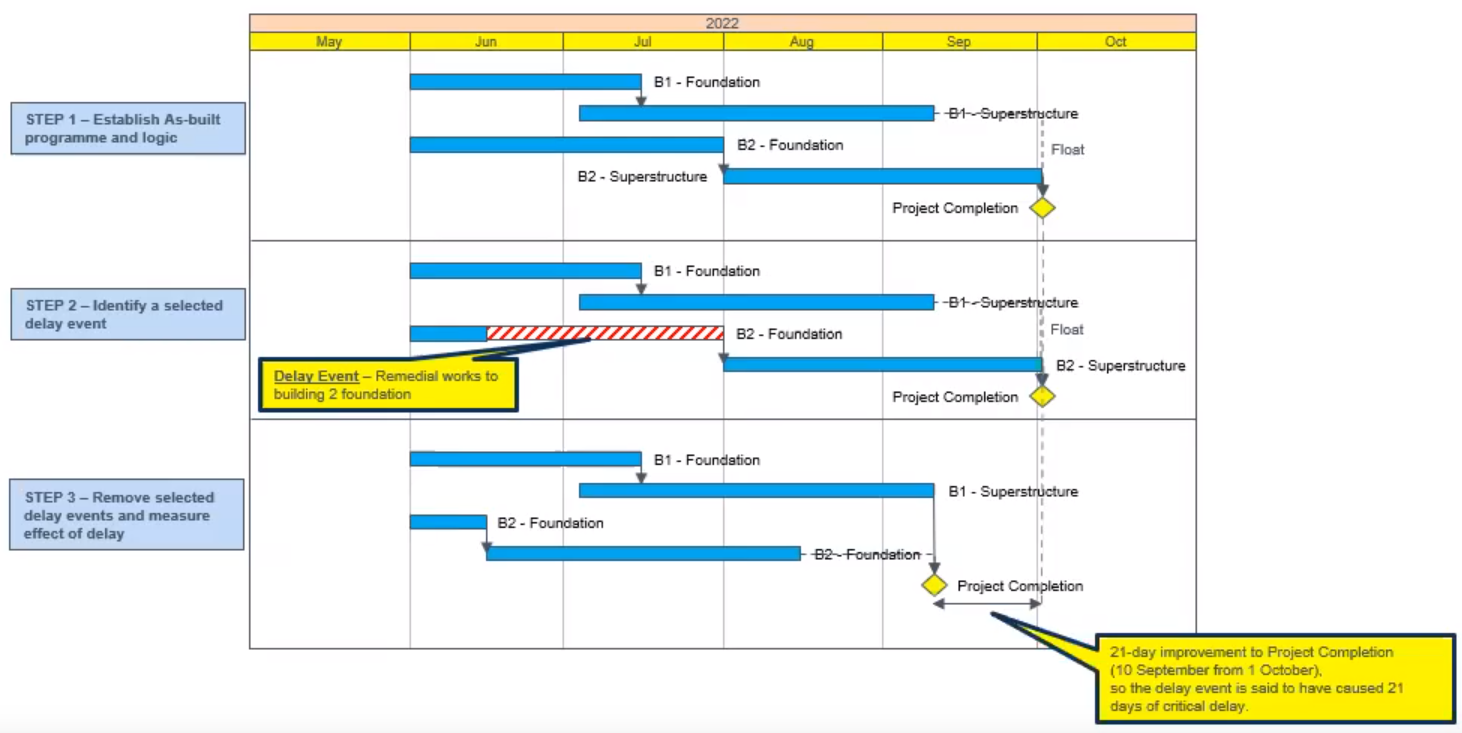
\includegraphics[width = \textwidth]{img/figure45.png}
    \caption{Collapsed as-built analysis for example project.}
\end{figure}
\subsection{Why so many methods?}
Blame lawyers and claims consultants.
\begin{table}[H]
    \centering
    \begin{tabular}{@{}ll@{}}
        \toprule
        \textbf{Method of analysis}             & \textbf{The question it answers}                                           \\
        \midrule
        Impacted as-planned analysis            & What effect would this event(s) have had on the completion date            \\
                                                & assuming everything else went exactly as planned in the programme?         \\
        Time impact analysis                    & What was the likely effect of this event(s) on the completion date         \\
                                                & adjudged from the point in time it was instructed or arose?                \\
        Time slice windows analysis             & What was the contemporaneous or actual critical path to completion         \\
                                                & throughout the works and what were the causes of delay thereto?            \\
        As-planned vs as-built windows analysis & What was the contemporaneous or actual critical path to completion         \\
                                                & throughout the works and what were the causes of delay?                    \\
        Longest path analysis                   & What was the as-built critical path to completion, viewed retrospectively, \\
                                                & and what were the causes of delay thereto?                                 \\
        Collapsed as-built analysis             & But for the event(s) when would the completion date have been achieved?    \\
        \bottomrule
    \end{tabular}
    \caption{Justification for various methods of analysis.}
\end{table}
\subsection{Example 2}
\begin{figure}[H]
    \centering
    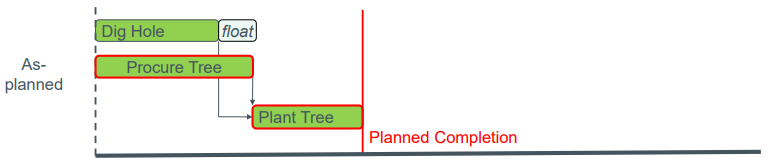
\includegraphics[width = \textwidth]{img/figure46.png}
    \caption{A simple project programme.}
\end{figure}
\begin{figure}[H]
    \centering
    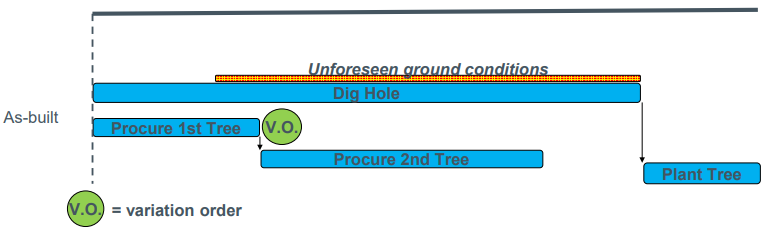
\includegraphics[width = \textwidth]{img/figure47.png}
    \caption{Actual programme.}
\end{figure}
\begin{figure}[H]
    \centering
    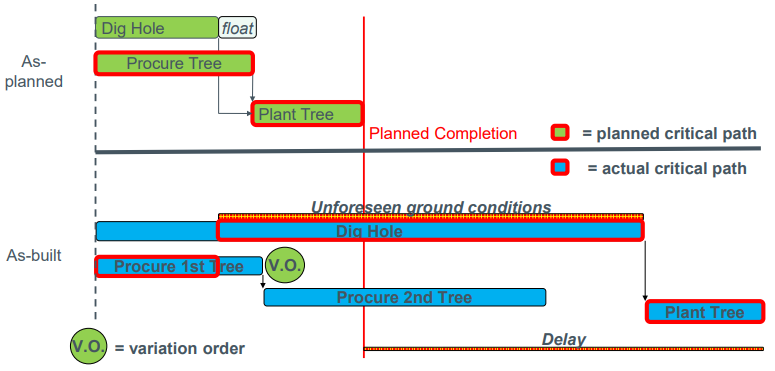
\includegraphics[width = \textwidth]{img/figure48.png}
    \caption{Comparison between planned and actual programmes.}
\end{figure}
Then the unhappy, but clever, instructing lawyer thinks:
\begin{quoting}
    ``That's all very well Mr Delay Expert, but what about the classic `but' for test of causation? Has there been an act of prevention here?''
\end{quoting}
\begin{figure}[H]
    \centering
    \includegraphics[width = \textwidth]{img/figure49.png}
    \caption{Critical path analysis.}
\end{figure}
\begin{figure}[H]
    \centering
    \includegraphics[width = \textwidth]{img/figure50.png}
    \caption{But-for delay.}
\end{figure}
\begin{quoting}
    ``Your honour, as a consequence of the instructed VO, there were no circumstances where my client could have completed this project any earlier than X. It would be harsh, indeed immoral, to expose her to Liquidated Damages liability before that date!''
\end{quoting}
\begin{figure}[H]
    \centering
    \includegraphics[width = \textwidth]{img/figure51.png}
    \caption{Reduced exposure to liquidated damages.}
\end{figure}
\section{Summary}
\begin{enumerate}
    \item The \textbf{delay expert} advises how the project was delayed
    \item The \textbf{technical expert} advises what technically went wrong
    \item The \textbf{quantum expert} advise on additional costs
    \item The \textbf{court} assigns liability and ultimately extension of time and damages
\end{enumerate}
\chapter{Financial Project Planning}
\section{Budgeting}
\subsection{What is budgeting?}
Budgeting involves examining:
\begin{itemize}
    \item Estimated revenues
    \item Estimated expenditures
\end{itemize}
over a specific period in the future, to determine a prediction of future company performance.
\subsection{What information is used for budgeting?}
\begin{enumerate}
    \item Accounting records
    \item Other sources within the company e.g. engineering / sales / production teams
    \item Sources outside the company e.g. published information, personal contacts
    \item Research and development
\end{enumerate}
in decreasing order of importance (approximately).
\subsection{Types of budget}
\begin{enumerate}
    \item Master budget: aggregation of lower-level budgets
    \item Operating budget: ``projected income statement''
    \item Cash budget: ``cash flow forecast''
    \item Capital budget: ``projected balance sheet''
    \item Labour budget: ``Staffing forecast''
    \item Static budget: fixed revenue and expenses
\end{enumerate}
\subsection{Example 1: Operating budget}
Deere Consulting Ltd. has the following income statement for 2021:
\begin{table}[H]
    \centering
    \begin{tabular}{@{}lr@{}}
        \toprule
        \textbf{Revenue}            & \textbf{\pounds (,000)} \\
        \midrule
        Sales                       & 25,323                  \\
        Cost of goods sold          & 18,582                  \\
        \midrule
        Gross profit                & 6,741                   \\
        \midrule
        \textbf{Operating expenses} &                         \\
        \midrule
        Total operating expenses    & 5,223                   \\
        \midrule
        Net income                  & 1,280                   \\
        \bottomrule
    \end{tabular}
    \caption{Deere Consulting Ltd. Income Statement. Year ended 31 December, 2021.}
\end{table}
Deere Consulting Ltd. has provided the following supplementary information to further assist with the budget:
\begin{itemize}
    \item Operating expenses are expected to increase to \pounds 5.62 million and sales are expected to increase proportionally
    \item The gross profit margin is expected to remain unchanged
\end{itemize}
Currently:
\begin{gather}
    \frac{\textrm{Sales}}{\textrm{Op. Ex}} = \frac{25323}{5223} = 4.85\\
    \textrm{Gross profit margin} = \frac{\textrm{Gross profit}}{\textrm{Sales}} = \frac{6741}{25323} = 26.6\%
\end{gather}
\begin{table}[H]
    \centering
    \begin{tabular}{@{}lr@{}}
        \toprule
        \textbf{Revenue}            & \textbf{\pounds (,000)} \\
        \midrule
        Sales                       & 27,257                  \\
        Cost of goods sold          & 20,007                  \\
        \midrule
        Gross profit                & 7,250                   \\
        \midrule
        \textbf{Operating expenses} &                         \\
        \midrule
        Total operating expenses    & 5,620                   \\
        \midrule
        Net income                  & 1,360                   \\
        \bottomrule
    \end{tabular}
    \caption{Deere Consulting Ltd. Income Statement. Year ended 31 December, 2022.}
\end{table}
\section{Cash flow forecast}
Cash flow forecasts are useful for clarifying the consequences of flows of money that occur at various times.
\begin{gather}
    \textrm{Net Cash Flow over time } t =\\
    \sum \textrm{Cash inflows in $t$} - \sum \textrm{Cash outflows in $t$}
\end{gather}
Cash flow forecasts are important because they form the basis of evaluating alternative projects.

Cash flow diagrams can be used to visualise flows of money that occur at various times.
\begin{figure}[H]
    \centering
    \includegraphics[width = 0.8\textwidth]{img/figure52.png}
    \caption{Cash flow forecast.}
\end{figure}
\begin{figure}[H]
    \centering
    \includegraphics[width = 0.8\textwidth]{img/figure53.png}
    \caption{Cash flow forecast.}
\end{figure}
\subsection{Example 2}
Before evaluating the economic merits of a proposed investment, the ABC corporation insists that its engineers develop a cash-flow diagram of the proposal. An investment of \pounds 10,000 can be made that will produce uniform annual revenue of \pounds 5,310 for five years and then have a market (recovery) value of \pounds 2,000 at the EOY five. Annual expenses will be \pounds 3,000 at the end of each year for operating and maintaining the project.
\begin{quoting}
    Draw a cash-flow diagram for the five-year life of the project. Use the corporation's viewpoint
\end{quoting}
\begin{figure}[H]
    \centering
    \includegraphics[width = 0.8\textwidth]{img/figure55.png}
    \caption{Cash flow diagram for ABC corporation.}
\end{figure}
So far, we have neglected the time value of money.
\begin{figure}[H]
    \centering
    \includegraphics[width = 0.8\textwidth]{img/figure54.png}
    \caption{Time value of money in cash flow forecast.}
\end{figure}
\subsection{Time value of money}
Remember the formula for PV:
\begin{equation}
    PV = \frac{FV}{\left(1+i\right)^n}
\end{equation}
Present value (PV) of future value (FV) in $n$ periods, for an interest rate $i$.

Remember the formula for AV:
\begin{equation}
    AV = PV \frac{i\left(1 + i\right)^n}{\left(1+i\right)^n - 1}
\end{equation}
Value of a series of uniform (annual) receipts (AV) that occur at the end of periods 1 to $n$, given their present value (PV) and an interest rate $i$.
\subsection{Example 3}
A processing plant is considering the installation of a newly designed solar energy system that will power the majority of its energy operations, and sell \pounds 450,000 per year of surplus energy to the grid over its expected lifetime of 10 years. If the interest rate is 12\% per year, how much money can the plant afford to invest in the new boiler system?
\begin{figure}[H]
    \centering
    \includegraphics[width = 0.8\textwidth]{img/figure56.png}
    \caption{Cash flow diagram. Example 3.}
\end{figure}
\begin{gather}
    i = 0.12 \qquad n = 10\\
    PV = AV \frac{\left(1 + i\right)^n - 1}{i\left(1+i\right)^n}\\
    PV = 450000\times \frac{\left(1 + 0.12\right)^{10} - 1}{0.12\left(1+ 0.12\right)^{10}}\\
    PV = \pounds 2,542,600
\end{gather}
which is the upper limit on what the plant can afford to spend on the steam system.
\subsection{Example 4}
Automotive Engineering Ltd. is required to pay money into a compensatory fund, to cover damages caused by a company-related accident. The company will pay in \pounds 3 billion at the end of the third quarter of 2022 and another \pounds 2 billion in the fourth quarter of 2022. Twelve additional payments of \pounds 1.25 billion each quarter thereafter will result in a total of \pounds 20 billion having been paid into the fund. The interest rate is 3\% per quarter.
\begin{quoting}
    What will be the value of this payment stream at the beginning of the third quarter of 2022?
\end{quoting}
\begin{figure}[H]
    \centering
    \includegraphics[width = 0.8\textwidth]{img/figure57.png}
    \caption{Cash flow diagram. Example 4.}
\end{figure}
PV of first end-of-quarter payment (\pounds 3 billion):
\begin{gather}
    \frac{3}{\left(1+0.03\right)^1} = \pounds 2.91\textrm{b}
\end{gather}
PV of second end-of-quarter payment (\pounds 2 billion):
\begin{gather}
    \frac{2}{\left(1+0.03\right)^2} = \pounds 1.89\textrm{b}
\end{gather}
FV of subsequent end-of-quarter payment (\pounds 1.25 billion):
\begin{gather}
    1.25\times \frac{\left(1+0.03\right)^{12}-1}{0.03\left(1+0.03\right)^{12}} = \pounds 12.44\textrm{b}
\end{gather}
PV of subsequent end-of-quarter payment (\pounds 1.25 billion):
\begin{gather}
    \frac{12.44}{\left(1+0.03\right)^2} = \pounds 11.73\textrm{b}
\end{gather}
PV of payment stream:
\begin{gather}
    2.91 + 1.89 + 11.73 = \pounds 16.53\textrm{b}
\end{gather}
\subsection{Cash flow forecast: table}
Cash flow tables are useful when the complexity of a situation makes it difficult to show all cash-flow amounts on a diagram. Cash flow tables can facilitate the analysis of different plans and designs. Cash flow tables clarify:
\begin{enumerate}
    \item The timing of cash flows
    \item The assumptions being made
    \item The amount of data available
\end{enumerate}
\subsection{Example 5}
CEGE Ltd. is renovating its office building and have identified two feasible alternatives for upgrading the heating, ventilation and air conditioning (HVAC) system. Either alternative A or alternative B must be implemented. The costs are as follows.
\begin{table}[H]
    \centering
    \begin{tabular}{@{}lr@{}}
        \toprule
        Equipment, labour and materials to rebuild & \pounds 18,000 \\
        Annual cost of electricity                 & \pounds 32,000 \\
        Annual maintenance expenses                & \pounds 2,400  \\
        Estimated market value (after eight years) & \pounds 2,000  \\
        \bottomrule
    \end{tabular}
    \caption{Alternative A: Rebuild (overhaul) the existing HVAC system.}
\end{table}
\begin{table}[H]
    \centering
    \begin{tabular}{@{}lr@{}}
        \toprule
        Equipment, labour and materials to rebuild     & \pounds 60,000 \\
        Annual cost of electricity                     & \pounds 9,000  \\
        Annual maintenance expenses                    & \pounds 16,000 \\
        Replacement of a major component in four years & \pounds 9,400  \\
        Estimated market value (after eight years)     & \pounds 8,000  \\
        \bottomrule
    \end{tabular}
    \caption{Alternative B: Install a new HVAC system that uses existing equipment.}
\end{table}
Assume that both alternatives will provide equivalent services over an eight-year period.
\begin{quoting}
    Use a cash flow table to tabulate the net cash flows for both alternatives.
\end{quoting}
\begin{quoting}
    Determine the annual net cash flow difference between the alternatives (B-A).
\end{quoting}
\begin{table}[H]
    \centering
    \begin{tabular}{@{}lllll@{}}
        \toprule
                    & \textbf{Alternative A}  & \textbf{Alternative B}  & \textbf{Difference} & \textbf{Cumulative}  \\
        End of year & Net cash flow (\pounds) & Net cash flow (\pounds) & B-A (\pounds)       & Difference (\pounds) \\
        \midrule
        0           & -18,000                 & -60,000                 & -42,000             & -42,000              \\
        1           & -34,400                 & -25000                  & 9,400               & -32,600              \\
        2           & -34,400                 & -25000                  & 9,400               & -23,200              \\
        3           & -34,400                 & -25000                  & 9,400               & -13,800              \\
        4           & -34,400                 & -34400                  & 0                   & -13,800              \\
        5           & -34,400                 & -25000                  & 9,400               & -4,400               \\
        6           & -34,400                 & -25000                  & 9,400               & 5,000                \\
        7           & -34,400                 & -25000                  & 9,400               & 14,400               \\
        8           & -32,400                 & -17000                  & 15,400              & 29,800               \\
        \midrule
        Total       & -291,200                & -261,400                &                     & 29,800               \\
        \bottomrule
    \end{tabular}
    \caption{Example 5 table.}
\end{table}
Some important notes:
\begin{itemize}
    \item Timing is everything
          \begin{itemize}
              \item When is money being received?
              \item When is money being paid?
          \end{itemize}
    \item Cash flows deal with expected actual receipts and payments
          \begin{itemize}
              \item Debtors and creditors (from the balance sheet) do not appear
          \end{itemize}
    \item Cash flow forecasts can act as an early warning system
          \begin{itemize}
              \item Can help identify the need for a loan or overdraft far in advance
          \end{itemize}
\end{itemize}
\section{S-curves}
Display cumulative data (costs, hours, quantities etc.) for a project.
\begin{figure}[H]
    \centering
    \includegraphics[width = 0.5\textwidth]{img/figure59.png}
    \caption{S-curve.}
\end{figure}
\subsection{What are s-curves used for?}
Resource allocation planning:
\begin{itemize}
    \item S-curves of expected person-hours versus time shows how the project team will need to flex over the project lifecycle
    \item This can aid the recruitment process
\end{itemize}
Project expenditure:
\begin{itemize}
    \item S-curves can show planned expenditure over the project time period
    \item If this is overlaid with information on when project funds are expected, cash flow problems can be identified
\end{itemize}
\subsection{Why are s-curves useful?}
S-curves can be used to compare real-time and projected progress.
\begin{figure}[H]
    \centering
    \includegraphics[width = 0.5\textwidth]{img/figure60.png}
    \caption{S-curve with real-time and projected progress.}
\end{figure}
\begin{itemize}
    \item S-curves help you to predict when resources will be heavily utilised
    \item S-curves help you manage stakeholder expectations
    \item S-curves help you plan for different schedule scenarios
\end{itemize}
\subsection{Example 6}
The ABC Corporation is planning a construction project with monthly projected receipts and expenditures as presented in the table below.
\begin{table}[H]
    \centering
    \small
    \setlength\tabcolsep{2pt}
    \begin{tabularx}{\textwidth}{@{}llllllllllllll@{}}
        \toprule
        \multicolumn{14}{l}{\textbf{ABC Corporation Construction Project}}                                                                                  \\
        \midrule
        Month                  & 1      & 2       & 3      & 4      & 5       & 6       & 7       & 8       & 9      & 10      & 11     & 12      & 13      \\
        Projected total        & 0      & 186,861 & 0      & 0      & 373723  & 0       & 0       & 0       & 0      & 934,307 & 0      & 186,861 & 186,861 \\
        receipts (\pounds)     &        &         &        &        &         &         &         &         &        &         &        &                   \\
        Projected total        & 30,000 & 114,338 & 50,000 & 40,062 & 110,396 & 200,000 & 200,000 & 441,535 & 55,215 & 55,675  & 40,000 & 40,000  & 0       \\
        expenditures (\pounds) &        &         &        &        &         &         &         &         &        &         &        &                   \\
        \bottomrule
    \end{tabularx}
    \caption{Example 6 table.}
\end{table}
\begin{figure}[H]
    \centering
    \includegraphics[width = 0.8\textwidth]{img/figure61.png}
    \caption{S-curve for example 6.}
\end{figure}
\begin{figure}[H]
    \centering
    \includegraphics[width = 0.8\textwidth]{img/figure62.png}
    \caption{S-curve for example 6 with cash flow analysis.}
\end{figure}
\section{Summary}
\begin{itemize}
    \item Budgeting
          \begin{itemize}
              \item Definition of budgeting
              \item Description of budget types
              \item Demonstration of an operating budget
          \end{itemize}
    \item Cash flow forecasts
          \begin{itemize}
              \item Description of cash flow diagrams
              \item Description of cash flow tables
              \item Demonstrations of cash flow diagrams and tables
          \end{itemize}
    \item S-curves
          \begin{itemize}
              \item Description of s-curves
              \item Uses of s-curves
              \item Demonstration of constructing an s-curve for expenditure
          \end{itemize}
\end{itemize}
\chapter{Project Risk Analysis}
\section{What is risk?}
Risk is a condition where there is a possibility of adverse deviation from a desired and expected outcome. Risk is caused by a lack of precise knowledge regarding future business conditions, technological development, synergies among projects etc. Decisions under risk are decisions in which the analyst models the decision problem in terms of assumed possible future outcomes, or scenarios, whose probabilities of occurrence can be estimated.
\subsection{Sources of uncertainty}
Factors that affect uncertainty in modelling future economic consequences of an engineering project are:
\begin{itemize}
    \item Possible inaccuracy of the cash-flow estimates
    \item The type of business involved in relation to the future health of the economy
    \item The type of physical plant and equipment involved
    \item Length of the study period used
\end{itemize}
\section{Measuring risk}
\subsection{Random variables}
Factors that have probabilistic outcomes (e.g., sots, revenues, useful life) are called random variables. Capital letters $X$, $Y$, $Z$, are usually used to represent random variables and lowercase letters $x$, $y$, $z$ are used to denote the particular values these variables take on in the \textit{sample space}\footnote{Sample space: the set of all possible outcomes for each variable.}. Information about random variables that is particularly helpful for risk analysis is their expected value and variances. Random variables can be defined as either discrete or continuous.
\subsection{Discrete random variables}
A random variable $X$ is said t o be discrete if it can take on at most a countable (finite) number of values ($x_1, x_2, \dots, x_L$). The probability that a discrete random variable $X$ takes on the value $x_i$ is given by:
\begin{equation}
    \textrm{Pr} \left\{X = x_i \right\} = P\left(x_i\right) \textrm{ for } i = 1,2,\dots , L
\end{equation}
where $i$ is the sequential index of the discrete values and $p\left(x_i\right) \geq 0$ and $\sum_i p\left(x_i\right) = 1$.

The probability that the value of $X$ is contained in the closed interval $\left[a,b\right]$ is given by the probability mass function:
\begin{equation}
    \textrm{Pr} \left\{ a \leq X \leq b \right\} = \sum_{ i:a\leq X_i \leq b } p\left(x_i\right)
\end{equation}
The probability that the value of $X$ is less than or equal to $h$ is given by the cumulative distribution function:
\begin{equation}
    \textrm{Pr} \left\{ X \leq h\right\} = p\left(h\right) = \sum_{i:X_i\leq h} p\left(x_i\right)
\end{equation}
In most practical cases, discrete random variables represent countable data such as:
\begin{itemize}
    \item The number of defective columns in a building
    \item The number of maintenance jobs per week
    \item The number of employees
\end{itemize}
\subsection{Continuous random variables}
A random variable $X$ is said to be continuous if it can take on any value within a set of real number $\left[c,d\right]$. The probability that a continuous random variable $X$ takes on a value within the set $\left[c,d\right]$ is given by:
\begin{equation}
    \textrm{Pr}\left\{c\leq X \leq d\right\} = \int_c^d f\left(x\right)\dif x
\end{equation}
where $\int_{\infty}^{\infty}f\left(x\right)\dif x = 1$.

The probability that the value of $X$ assumes exactly any one of its values is 0. The probability that the value of $X$ is less than or equal to $h$ is given by the cumulative distribution function:
\begin{align}
    \textrm{Pr}\left\{X\leq h\right\}         & = F\left(h\right) = \int_{-\infty}^h f\left(x\right)\dif x            \\
    \textrm{Pr}\left\{c \leq X \leq d\right\} & = \int_c^d f\left(x\right) \dif x = F\left(d\right) - F\left(c\right)
\end{align}
In most practical cases, continuous random variables represent measured data such as:
\begin{itemize}
    \item Time
    \item Cost
    \item Revenue
\end{itemize}
\subsection{Expected value}
The expected value of a random variable $X$ is denoted as $E\left(X\right)$. $E\left(X\right)$ is a weighted average of the distribution values of $x$ that it takes on and is a measure of the central location of the distribution. $E\left(X\right)$ is called the mean (or central / first moment) of the distribution.

For a discrete random variable:
\begin{equation}
    E\left(X\right) = \sum_i x_i p\left(x_i\right)
\end{equation}
For a continuous random variable:
\begin{equation}
    E\left(X\right) = \int_{-\infty}^{\infty} x f\left(x\right)\dif x
\end{equation}
\subsection{Variance}
The variance of a random variable $X$ is denoted as $V\left(X\right)$. $V\left(X\right)$ is a measure of the dispersion of the values $X$ takes on around $E\left(X\right)$ (note that the square root of $V\left(X\right)$ is equal to the standard deviation $SD\left(X\right)$). $V\left(X\right)$ is called the second moment of the distribution.

For a discrete random variable:
\begin{equation}
    V\left(X\right) = \sum_i \left[x_i - E\left(X\right)\right]^2 p\left(x_i\right)
\end{equation}
For a continuous random variable:
\begin{equation}
    V\left(X\right) = \int_{-\infty}^{\infty} \left[x - E\left(X\right)\right]^2 f\left(x\right) \dif x
\end{equation}
\subsection{Multiplying by a constant}
Random variables are commonly multiplied by a constant value. e.g.:
\begin{itemize}
    \item The estimated maintenance labour expense for a time period $Y = cX$, where the number of labour hours per period is a random variable $X$ and the cost per labour hour $c$ is constant.
\end{itemize}
For a discrete random variable:
\begin{equation}
    E\left(cX\right) = cE\left(X\right) = c\sum_i x_i p\left(x_i\right)
\end{equation}
For a continuous random variable:
\begin{equation}
    E\left(cX\right) = cE\left(X\right) = c \int_{-\infty}^{\infty} x f\left(x\right) \dif x
\end{equation}
For both random variable types:
\begin{equation}
    V\left(cX\right) = c^2 V\left(X\right)
\end{equation}
\subsection{Multiplying by another random variable}
Sometimes a random variable $Z$ results from the product of two other independent random variable $(XY)$, e.g.:
\begin{itemize}
    \item The estimated annual expenses $Z$ for a repair part repetitively procured during the year on a competitive basis, when the unit price $X$ and the number of units used per year $Y$ are independent random variables.
\end{itemize}
The expected value of $Z$ is:
\begin{equation}
    E\left(Z\right) = E\left(X\right)E\left(Y\right)
\end{equation}
The variance of $Z$ is:
\begin{equation}
    V\left(Z\right) = E\left[XY - E\left(XY\right)\right]^2 = E\left(X^2\right)E\left(Y^2\right)- \left[E\left(X\right)E\left(Y\right)\right]^2
\end{equation}
\subsection{Adding or subtracting random variables}
Sometimes a random variable (Z) results from adding or subtracting two independent variables ($X+Y$ or $X-Y$) e.g.:
\begin{itemize}
    \item Alternative A has a cost of $X$ and alternative B has a cost of $Y$. The probability that alternative A is less costly than alternative B is equal to:
          \begin{equation}
              \textrm{Pr}\left\{X < Y \right\} = \textrm{Pr}\left\{ X-Y < 0\right\} = \textrm{Pr} \left\{ Z < 0\right\}
          \end{equation}
\end{itemize}
The expected value of $Z$ is:
\begin{equation}
    E\left(Z\right) = E\left(X\right) \pm E\left(Y\right)
\end{equation}
The variance of $Z$ is:
\begin{equation}
    V\left(Z\right) = V\left(X\right) + V\left(Y\right)
\end{equation}
\section{Example risk analysis}
\subsection{Worked example 1}
Suppose that the estimated probability of obtaining various capacity utilisations in a premixed-concrete plant project are as follows:
\begin{table}[H]
    \centering
    \begin{tabular}{@{}llll@{}}
        \toprule
        \textbf{Capacity (\%)} & \textbf{Probability} & \textbf{Annual Revenue} & \textbf{AV (15\%)} \\
        \midrule
        50                     & 0.10                 & \pounds 405,000         & -\pounds 25,093    \\
        65                     & 0.30                 & \pounds 526,500         & \pounds 22,136     \\
        75                     & 0.50                 & \pounds 607,500         & \pounds 53,622     \\
        90                     & 0.10                 & \pounds 729,000         & \pounds 100,850    \\
        \bottomrule
    \end{tabular}
    \caption{Worked example 1 table.}
\end{table}
\begin{quoting}
    Estimate $E\left(AV\right)$ and $V\left(AV\right)$
\end{quoting}
\begin{gather}
    E\left(X\right) = \sum_i x_i p\left(x_i\right)\\
    E\left(AV\right) = 0.1 \times -25903 + 0.3 \times 22136 + 0.5 \times 53622 + 0.1 \times 100850 = \pounds 41,028\\
    V\left(X\right) = \sum_i \left[x_i - E\left(X\right)\right]^2 p\left(x_i\right)
\end{gather}
\begin{multline}
    V\left(AV\right) = 0.1 \times \left(-25903 - 41028\right)^2 + 0.3 \times \left(22136 - 41028\right)^2 + \\
    0.5 \times \left(53622 - 41028\right)^2 + 0.1 \times \left(100850 - 41028\right)^2 = \pounds\SI{9.9e8}{}
\end{multline}
\begin{align}
    E\left(AV\right)        & = \pounds 41,028       \\
    V\left(AV\right)        & = \pounds \SI{9.9e8}{} \\
    \sqrt{V\left(AV\right)} & = \pounds 31,327
\end{align}
By evaluating both $E\left(AV\right)$ and $V\left(AV\right)$ for the concrete plant, indications of the venture's average profitability and riskiness are obtained. The mean value is above one standard deviation from \pounds 0. This leads to the conclusion that there is low risk, and that this is a good investment.
\subsection{Risk analysis with continuous random variables}
Supposed that the NPV of a project is \pounds 153 and the corresponding variance is \pounds 484,416. If the NPV is a normally distributed\footnote{Commonly used distribution that is easy to calculate using a computer and can be entirely described by the mean and variance parameters.} random variable, what is the probability of having a negative NPV?

From Excel, use \texttt{=norm.dist(0,E(NPV),sqrt(V(NPV)),1)}. The first value is 0, because we want to find the probability of it being less than the mean. The last 1 gives us the cumulative distribution. This results in a 41.3\% of having a NPV less than 0.
\begin{equation}
    \textrm{Pr}\left\{ NPV \leq 0\right\} = F(0) = \int_{-\infty}^0 f\left(npv\right)\dif npv = 0.413
\end{equation}
\subsection{Risk analysis with multiple independent random variables}
Suppose that the estimated cash flow data for a project are show in the following table for a five-year study period. Each annual net cash-flow amount, $F_k$, is a linear combination of two statistically independent random variables, $X_k$ and $Y_k$, where $X_k$ is a revenue factor and $Y_k$ is an expense factor. The $X_k$ cash-flow amounts are statistically independent of each other, and the same is true of the $Y_k$ amounts. Both $X_k$ and $Y_k$ are continuous random variables, but the form of their probability distributions is not known. Interest rate is 20\% per year.
\begin{quoting}
    Estimate $E\left(NPV\right)$, $V\left(NPV\right)$ and $SD\left(NPV\right)$ of the project's cash flows.
\end{quoting}
\begin{table}[H]
    \centering
    \begin{tabular}{@{}llllll@{}}
        \toprule
        \textbf{End of year} $k$ & \textbf{Net cash flow} & $E\left[X_k\right]$ & $E\left[Y_k\right]$ & $SD\left[X_k\right]$ & $SD\left[Y_k\right]$ \\
        \midrule
        0                        & $F_0 = X_0 + Y_0$      & \pounds 0           & -\pounds 100,000    & \pounds 0            & \pounds 10,000       \\
        1                        & $F_1 = X_1 + Y_1$      & \pounds 60,000      & -\pounds 20,000     & \pounds 4,500        & \pounds 2,000        \\
        2                        & $F_2 = X_2 + 2Y_2$     & \pounds 65,000      & -\pounds 15,000     & \pounds 8,000        & \pounds 1,200        \\
        3                        & $F_3 = 2X_3 + 3Y_3$    & \pounds 40,000      & -\pounds 9,000      & \pounds 3,000        & \pounds 1,000        \\
        4                        & $F_4 = X_4 + 2Y_4$     & \pounds 70,000      & -\pounds 20,000     & \pounds 4,000        & \pounds 2,000        \\
        5                        & $F_5 = 2X_5 + 2Y_5$    & \pounds 55,000      & -\pounds 18,000     & \pounds 4,000        & \pounds 2,300        \\
        \bottomrule
    \end{tabular}
    \caption{Risk analysis with multiple independent random variables table.}
\end{table}
\begin{align}
    E\left(F_k\right) & = E\left(a_k X_k + b_k Y_k\right) = E\left(a_k X_k\right) + E\left(b_k Y_k\right) = a_k E\left(X_k\right) + b_k E\left(Y_k\right)     \\
    V\left(F_k\right) & = V\left(a_k X_k + b_k Y_k\right) = V\left(a_k X_k\right) + V\left(b_k Y_k\right) = a_k^2 V\left(X_k\right) + b_k^2 V\left(Y_k\right)
\end{align}
\begin{table}[H]
    \centering
    \begin{tabular}{@{}llllllll@{}}
        \toprule
        \textbf{End of year} $k$ & \textbf{Net cash flow} & $E\left[X_k\right]$ & $E\left[Y_k\right]$ & $SD\left[X_k\right]$ & $SD\left[Y_k\right]$ & $E\left[F_k\right]$ & $V\left[V_k\right]$ \\
        \midrule
        0                        & $F_0 = X_0 + Y_0$      & \pounds 0           & -\pounds 100,000    & \pounds 0            & \pounds 10,000       & -\pounds 100,000    & \SI{100e6}{}        \\
        1                        & $F_1 = X_1 + Y_1$      & \pounds 60,000      & -\pounds 20,000     & \pounds 4,500        & \pounds 2,000        & \pounds 40,000      & \SI{24.2e6}{}       \\
        2                        & $F_2 = X_2 + 2Y_2$     & \pounds 65,000      & -\pounds 15,000     & \pounds 8,000        & \pounds 1,200        & \pounds 35,000      & \SI{69.8e6}{}       \\
        3                        & $F_3 = 2X_3 + 3Y_3$    & \pounds 40,000      & -\pounds 9,000      & \pounds 3,000        & \pounds 1,000        & \pounds 53,000      & \SI{45e6}{}         \\
        4                        & $F_4 = X_4 + 2Y_4$     & \pounds 70,000      & -\pounds 20,000     & \pounds 4,000        & \pounds 2,000        & \pounds 30,000      & \SI{32e6}{}         \\
        5                        & $F_5 = 2X_5 + 2Y_5$    & \pounds 55,000      & -\pounds 18,000     & \pounds 4,000        & \pounds 2,300        & \pounds 74,000      & \SI{85.2e6}{}       \\
        \bottomrule
    \end{tabular}
    \caption{Risk analysis with multiple independent random variables table with expected and variance values.}
\end{table}
\begin{align}
    E\left(NPV\right)  & = \sum_{k=0}^5 \dfrac{E\left(F_k\right)}{\left(1+i\right)^n} = \pounds 32,517             \\
    V\left(NPV\right)  & = \sum_{k=0}^5 \dfrac{V\left(F_k\right)}{\left(1+i\right)^{2n}} = \pounds \SI{186.75e6}{} \\
    SD\left(NPV\right) & = \sqrt{V\left(NPV\right)} = \pounds 13,666
\end{align}
\section{Decision trees}
Decision trees are powerful means of depicting and facilitating the analysis of important problems. Decision tress break down a large, complicated problem into a series of smaller, simple problems. They enable objective analysis and decision making that includes explicit consideration of the risk and effect of the future.
\begin{figure}[H]
    \centering
    \includegraphics[width = 0.7 \textwidth]{img/figure63.png}
    \caption{Decision tree.}
\end{figure}
\subsection{Worked example of a decision tree}
CEGE Corporation manufactures compressors for commercial air-condition systems. A new compressor design is being evaluated as potential replacement for the most frequently used unit. The new design involves major changes that have the expected advantage of better operating efficiency. From the perspective of a typical user, the new compressor (as an assembled component in an air-conditioning system) would have an increased investment of \pounds 8,600 relative to the present unit and an annual expense saving dependent on the extent to which the design goal is met in actual operation. Estimates by the multidisciplinary design team of the new compressor achieving four levels (percentages) of the efficiency design goal and the probability and annual expense saving at each level are as follows.
\begin{table}[H]
    \centering
    \begin{tabular}{@{}lll@{}}
        \toprule
        \textbf{Level of design goal met (\%)} & \textbf{Probability} $p\left(L\right)$ & \textbf{Annual expense saving} \\
        \midrule
        90                                     & 0.25                                   & \pounds 3,470                  \\
        70                                     & 0.40                                   & \pounds 2,920                  \\
        50                                     & 0.25                                   & \pounds 2,310                  \\
        30                                     & 0.10                                   & \pounds 1,560                  \\
        \bottomrule
    \end{tabular}
    \caption{Decision tree example table.}
\end{table}
\begin{quoting}
    Use MARR = 18\%, an analysis period of 6 years, and $E\left(NPV\right)$ as the decision criterion, is the new compressor design economically preferable to the current unit?
\end{quoting}
Convert to present value figures using the formula for AV.
\begin{figure}[H]
    \centering
    \includegraphics[width = 0.5\textwidth]{img/figure64.png}
    \caption{Decision tree for worked example.}
\end{figure}
\begin{gather}
    E\left(X\right) = \sum_i x_i p\left(x\right)\\
    E\left(NPV\right) = 0.25 \times 3538 + 0.40 \times 1614 + 0.25\times (-520) + 0.10 \times (-3413) = 1086
\end{gather}
There is a 35\% chance of a negative NPV value, hence depending on the risk appetite of the company, we find that this may not be a good investment. However, we do have a positive $E\left(NPV\right)$ value.

%\newpage
%\bibliographystyle{unsrtnat}
%\bibliography{Refs.bib}
%\appendix
\chapter{Plots}
\begin{figure}[H]
    \centering
    \includegraphics[width = 0.8\textwidth]{img/Roll Type.pdf}
    \caption{RMSE results for Type-1 and Type-2 Configurations for Roll Output}
    \label{fig:roll_type}
\end{figure}
\begin{figure}[H]
    \centering
    \includegraphics[width = 0.8\textwidth]{img/Pitch Type.pdf}
    \caption{RMSE results for Type-1 and Type-2 Configurations for Pitch Output}
    \label{fig:pitch_type}
\end{figure}
\begin{figure}[H]
    \centering
    \includegraphics[width = 0.6\textwidth]{img/Yaw Type2.pdf}
    \caption{RMSE results for Type-1 and Type-2 Configurations for Yaw Output}
    \label{fig:yaw_type}
\end{figure}
\begin{figure}[H]
    \centering
    \includegraphics[width = 0.6\textwidth]{img/Thrust Type.pdf}
    \caption{RMSE results for Type-1 and Type-2 Configurations for Thrust Output}
    \label{fig:thrust_type}
\end{figure}
\begin{figure}[H]
    \centering
    \begin{minipage}[b]{0.45\textwidth}
        \includegraphics[height=5cm,keepaspectratio]{img/scenario1_pid_paths.eps}
        \caption{Scenario 1 Path taken using PID Drone Control}
        \label{fig:Paths1_pid}
    \end{minipage}
    \hfill
    \begin{minipage}[b]{0.45\textwidth}
        \includegraphics[height=5cm,keepaspectratio]{img/scenario1_fis_paths.eps}
        \caption{Scenario 1 Path taken using ANFIS Drone Control}
        \label{fig:Paths1_fis}
    \end{minipage}
\end{figure}
\begin{figure}[H]
    \centering
    \begin{minipage}[b]{0.45\textwidth}
        \includegraphics[height=5cm,keepaspectratio]{img/scenario2_pid_paths.eps}
        \caption{Scenario 2 Path taken using PID Drone Control}
        \label{fig:Paths2_pid}
    \end{minipage}
    \hfill
    \begin{minipage}[b]{0.45\textwidth}
        \includegraphics[height=5cm,keepaspectratio]{img/scenario2_fis_paths.eps}
        \caption{Scenario 2 Path taken using ANFIS Drone Control}
        \label{fig:Paths2_fis}
    \end{minipage}
\end{figure}
\begin{figure}[H]
    \centering
    \begin{minipage}[b]{0.45\textwidth}
        \includegraphics[height=5cm,keepaspectratio]{img/scenario3_pid_paths.eps}
        \caption{Scenario 3 Path taken using PID Drone Control}
        \label{fig:Paths3_pid}
    \end{minipage}
    \hfill
    \begin{minipage}[b]{0.45\textwidth}
        \includegraphics[height=5cm,keepaspectratio]{img/scenario3_fis_paths.eps}
        \caption{Scenario 3 Path taken using ANFIS Drone Control}
        \label{fig:Paths3_fis}
    \end{minipage}
\end{figure}
\begin{figure}[H]
    \centering
    \begin{minipage}[b]{0.45\textwidth}
        \includegraphics[height=5cm,keepaspectratio]{img/scenario4_pid_paths.eps}
        \caption{Scenario 4 Path taken using PID Drone Control}
        \label{fig:Paths4_pid}
    \end{minipage}
    \hfill
    \begin{minipage}[b]{0.45\textwidth}
        \includegraphics[height=5cm,keepaspectratio]{img/scenario4_fis_paths.eps}
        \caption{Scenario 4 Path taken using ANFIS Drone Control}
        \label{fig:Paths4_fis}
    \end{minipage}
\end{figure}
\begin{figure}[H]
    \centering
    \begin{minipage}[b]{0.45\textwidth}
        \includegraphics[height=5cm,keepaspectratio]{img/scenario5_pid_paths.eps}
        \caption{Scenario 5 Path taken using PID Drone Control}
        \label{fig:Paths5_pid}
    \end{minipage}
    \hfill
    \begin{minipage}[b]{0.45\textwidth}
        \includegraphics[height=5cm,keepaspectratio]{img/scenario5_fis_paths.eps}
        \caption{Scenario 5 Path taken using ANFIS Drone Control}
        \label{fig:Paths5_fis}
    \end{minipage}
\end{figure}

\end{document}